\documentclass[lettersize,journal]{IEEEtran}
\usepackage{amsmath,amsfonts}
\usepackage{algorithmic}
\usepackage{algorithm}
\usepackage{array}
\usepackage[caption=false,font=normalsize,labelfont=sf,textfont=sf]{subfig}
\usepackage{textcomp}
\usepackage{stfloats}
\usepackage{url}
\usepackage{verbatim}
\usepackage{graphicx}
\usepackage{cite}
\usepackage{booktabs}
\usepackage{wrapfig}
\usepackage[table,dvipsnames]{xcolor}
\usepackage{multicol}
\usepackage{tikz}
\usepackage{hyperref}
\usepackage[normalem]{ulem}
\usepackage{soul}
\usepackage{multirow}
\usepackage{amsmath,bm}
\usepackage{pifont}
\newcommand*\circled[1]{\tikz[baseline=(char.base)]{
            \node[shape=circle,draw,inner sep=0.4pt] (char) {#1};}}
\newcommand{\returnx}{\item\noindent{return}\ }

\newcommand{\hu}[1]{\stepcounter{todocounter}
  {\color{blue!90} #1}}
\newcommand{\ping}[1]{\textcolor{magenta}{#1}}
% \newcommand{}[1]{\textcolor{NavyBlue}{#1}}
\usepackage{orcidlink}
  
\hyphenation{op-tical net-works semi-conduc-tor IEEE-Xplore}
% updated with editorial comments 8/9/2021

\begin{document}

\title{Fed-HeLLo: Efficient Federated Foundation Model Fine-Tuning with Heterogeneous LoRA Allocation}

% \author{Anonymous Submission}

\author{Zikai Zhang\orcidlink{0009-0006-7437-6424},
Ping Liu\orcidlink{0000-0002-3170-3783},
Jiahao Xu\orcidlink{0000-0002-4888-252X},
Rui Hu*\orcidlink{0000-0003-3317-1765}
        % <-this % stops a space
% \thanks{This paper was produced by the IEEE Publication Technology Group. They are in Piscataway, NJ.}% <-this % stops a space
% \thanks{Manuscript received April 19, 2021; revised August 16, 2021.}
\thanks{Zikai Zhang, Ping Liu, Jiahao Xu, Rui Hu are with the Department of Computer Science and Engineering, University of Nevada, Reno, Reno, NV, 89557, USA (e-mail: zikaiz@unr.edu; pingl@unr.edu; jiahaox@unr.edu; ruihu@unr.edu).}
\thanks{*Rui Hu is the Corresponding Author: ruihu@unr.edu}
}

% The paper headers
\markboth{Journal of \LaTeX\ Class Files,~Vol.~14, No.~8, June~2025}%
{Shell \MakeLowercase{\textit{et al.}}: A Sample Article Using IEEEtran.cls for IEEE Journals}

% \IEEEpubid{0000--0000/00\$00.00~\copyright~2021 IEEE}
% Remember, if you use this you must call \IEEEpubidadjcol in the second
% column for its text to clear the IEEEpubid mark.

\maketitle

\begin{abstract}
Federated Learning (FL) has recently been utilized to collaboratively fine-tune foundation models (FMs) across multiple clients. Notably, federated low-rank adaptation (LoRA)-based fine-tuning methods have recently gained attention, which allows clients to fine-tune FMs with a small portion of trainable parameters locally. However, most existing methods do not account for the heterogeneous resources of clients or lack an effective local training strategy to maximize global fine-tuning performance under limited resources. In this work, we propose {Fed-HeLLo}, a novel federated LoRA-based fine-tuning framework that enables clients to collaboratively fine-tune an FM with different local trainable LoRA layers. To ensure its effectiveness, we develop several heterogeneous LoRA allocation (HLA) strategies that adaptively allocate local trainable LoRA layers based on clients' resource capabilities and the layer importance. 
Specifically, based on the dynamic layer importance, we design a Fisher Information Matrix score-based HLA (FIM-HLA) that leverages dynamic gradient norm information. To better stabilize the training process, we consider the intrinsic importance of LoRA layers and design a Geometrically-Defined HLA (GD-HLA) strategy. It shapes the collective distribution of trainable LoRA layers into specific geometric patterns, such as \textit{Triangle}, \textit{Inverted Triangle}, \textit{Bottleneck}, and \textit{Uniform}. Moreover, we extend GD-HLA into a randomized version, named Randomized Geometrically-Defined HLA (RGD-HLA), for enhanced model accuracy with randomness. By co-designing the proposed HLA strategies, we incorporate both the dynamic and intrinsic layer importance into the design of our HLA strategy.
To thoroughly evaluate our approach, we simulate various complex federated LoRA-based fine-tuning settings using five datasets and three levels of data distributions ranging from IID to extreme Non-IID. The experimental results demonstrate the effectiveness and efficiency of Fed-HeLLo with the proposed HLA strategies. The code is available at \url{https://github.com/TNI-playground/Fed_HeLLo}.
\end{abstract}

\begin{IEEEkeywords}
Foundation Model Fine-Tuning, Federated Learning, Low-Rank Adaptation, Resource Heterogeneity
\end{IEEEkeywords}

\section{Introduction}
\IEEEPARstart{F}{oundation} models (FMs)~\cite{dosovitskiy2020image, devlin2019bert, lyu2023attention, study2022, zhou2023comprehensive}, characterized by their extensive parameter counts ranging into millions or billions, serve as robust initial weights for a variety of downstream tasks~\cite{wu2023visual,wang2018glue} via fine-tuning. However, employing FMs presents substantial challenges, especially the high computational costs of fine-tuning the model.
% The foundation models (FMs)~\cite{dosovitskiy2020image, devlin2019bert, radford2021learning, bommasani2021opportunities, zhou2023comprehensive} are models with millions or even billions of parameters trained on large-scale datasets. They aim to provide powerful weight initialization for various downstream tasks across visual~\cite{wu2023visual}, language~\cite{wang2018glue}, and more. Numerous FMs~\cite{dosovitskiy2020image, devlin2019bert} have emerged recently, underscoring their exceptional adaptability and utility. Nonetheless, two significant challenges arise when employing FMs for downstream tasks: the substantial computational expenses associated with fully fine-tuning FMs and the privacy concerns regarding the collection of training data. 

To mitigate the high computational requirement of fine-tuning FMs, researchers have developed a variety of parameter-efficient fine-tuning (PEFT) methods. These methods either selectively update a subset of model parameters or incorporate a small set of trainable layers, such as in prompt tuning~\cite{lester2021power}, low-rank adaptation (LoRA)~\cite{hu2021lora}, and BitFit~\cite{zaken2022bitfit}.
% ~\cite{lester2021power, zaken2022bitfit, hu2021lora, he2021towards}
% {These methods can be categorized into three primary types: additive-based, selective-based, and re-parameterization-based.} While additive-based approaches like prompt-tuning~\cite{li2021prefix} offer noticeable reductions in computational costs, their {effectiveness} across {diverse} domains (e.g., visual tasks) remains {an open question}. 
% Selective-based methods~\cite{zaken2022bitfit} show inconsistent performance across different tasks in prior studies~\cite{ding2022delta}. 
% \ping{Given these factors}, we opt for the re-parameterization-based method, LoRA~\cite{hu2021lora}, \ping{which can offer consistent performance benefits while reducing computational and communication burdens~\cite{cho2023heterogeneous}.}
% 



Recent works~\cite{zhao2023fedprompt,guo2023promptfl,zhang2023towards,babakniya2023slora,sun2024improving} have started to explore the combination of FL and various PEFT methods due to their lightweight training structures. 
%
{Federated Learning (FL)~\cite{konecny2016federated,zawad2025fedcust} is a distributed machine learning framework that enables multiple clients to collaboratively update a global model.}
% without sharing their training data.
%
% FL training process, 
%
% PEFT 放在FL的好处：FL devices resource : peft parameter efficient--> computation and  communication benefit.
%
In the FL process, each client trains a local model on its private dataset and sends model updates to a central server for aggregation. Incorporating PEFT techniques in this process improves parameter efficiency, reducing both computational and communication overhead.
% during the process.
% For example, 
In the literature,
FedPrompt~\cite{zhao2023fedprompt} and PromptFL~\cite{guo2023promptfl} combine FL with prompt tuning, updating only the soft prompts to improve parameter and communication efficiency. Due to the advantages of LoRA in handling complex downstream tasks with mid-size dataset~\cite{zhang2023fedpetuning}, particularly those involving significant domain shifts, several studies have explored federated LoRA-based fine-tuning methods~\cite{zhang2023towards,babakniya2023slora}. 
% \ping{maybe we can move the following lines (L42-L45) to related works.} 
{For instance, FedIT~\cite{zhang2023towards} combines FL with LoRA for federated instruction-tuning. SLoRA~\cite{babakniya2023slora} introduces a novel initialization method for LoRA layers to improve the convergence speed of LoRA in FL.}
% FFA-LoRA~\cite{sun2024improving} enhances the privacy protection of the federated LoRA-based fine-tuning system using differential privacy.}

Despite advancements in federated LoRA-based fine-tuning, the persistent challenges are the memory bottlenecks experienced by clients with limited resources.
% when performing LoRA-based fine-tuning locally on clients with limited computational resources. 
While LoRA is designed to be parameter-efficient, it still requires substantial memory usage
% to store intermediate data like activations and optimizer states 
during training, similar to full-model fine-tuning~\cite{li2023fedtp}. 
As shown in Figure~\ref{fig:motivation} (a), the memory usage for training a ViT-base~\cite{krizhevsky2009learning} model
% with a 12-layer encoder and LoRA added to each layer 
including the memory for model parameters, optimizer states, and activations. The model parameters include the weights and biases of the frozen pre-trained model as well as trainable parameters.
%, using only 2.88\% of the memory. 
The optimizer states store gradients and necessary momentum estimates for trainable parameters.
% and take up 7.54\% of the memory. 
Activations are intermediate results in forward process that are stored for computing gradients in backpropagation. In this LoRA-based fine-tuning case, model parameters take only 3\% of the memory, while optimizer states and activations together take 97\% of the memory.

% 
% The model parameters memory takes around 
% 346 MB, the GPU context tasks around 513 MB.
% the optimizer requires around 904 MB of memory consumption, which is related to the number of trainable parameters, batch size, and the choice of optimizer (we use Adam in our case).
% In comparison, the footprints for activations and optimizer consume a significant portion of GPU memory of around 11645 MB. 
Furthermore, as shown in Figure~\ref{fig:motivation} (b), clients in real-world FL have heterogeneous memory capabilities, and the majority of them have low-resource devices with limited memory capabilities.
% Additionally, in Figure~\ref{fig:motivation} (b), we illustrate the distribution of heterogeneous devices in a federated learning system, showing that low-resource devices with limited GPU memory constitute the majority. 
This presents substantial challenges to the deployment of federated LoRA-based fine-tuning, as clients with limited memory resources are not capable of completing the local training task effectively and efficiently. 
% This can be a major issue for clients with constrained computational capabilities in a FL setting.
%
%
%
% Despite these advancements, one of the key challenges of federated LoRA-based fine-tuning remains unsolved: the memory bottleneck when performing LoRA-based fine-tuning locally on clients with limited computational resources. Although LoRA is parameter-efficient, it still requires extensive memory to store intermediate data for training, akin to full-model fine-tuning. This high memory consumption is especially problematic in FL, where clients usually have limited computational capabilities and may not be able to join the training. 
%
% To enable FL over clients with memory-constraint resources, as well as considering heterogeneous memory resources, vanilla methods have shown limitations~\cite{mitliagkas2016asynchrony,kim2022depthfl}. 
% For instance, 
In this case, FL usually assigns local training tasks only to high-capability clients (known as exclusive learning~\cite{kim2022depthfl}), which results in a significant loss of data from low-capability clients. Otherwise, FL conducts local training based on the resources of the least powerful client (known as straggler learning~\cite{mitliagkas2016asynchrony}). This is sub-optimal because it wastes the resources of high-capability clients that could perform more computation. 
% In contrast, exclusive learning~\cite{kim2022depthfl} allocates training tasks only to high-capability clients, resulting in a significant loss of data from low-capability clients. 
% These limitations also apply to federated LoRA-based fine-tuning scenarios. 
% Directly applying these methods to federated LoRA-based fine-tuning scenarios also result in resource or data wasting.
% It is challenging to fully leverage the diverse data and heterogeneous computational resources of clients simultaneously while guaranteeing the effectiveness and high performance of in LoRA-based fine-tuning. 
% Directly applying these methods to federated LoRA-based fine-tuning scenarios can lead to resource or data waste. Effectively utilizing diverse client data and heterogeneous memory resources while guaranteeing the effectiveness and high-performance LoRA-based fine-tuning remains challenging.


% To address the memory-constraint issue, existing works~\cite{su2023fedra,cho2023heterogeneous,wang2024flora,bai2024flexlora} \hl{on LoRA-based fine-tuning apply trainable LoRA layers to each transformer layer.} 
To address the memory constraint issue in heterogeneous resource settings,
existing works~\cite{su2023fedra,cho2023heterogeneous,wang2024flora,bai2024flexlora} employ training strategies where resource-limited clients use LoRA with smaller ranks~\cite{cho2023heterogeneous,wang2024flora,bai2024flexlora} or update
only partial
% only a subset of 
LoRA layers~\cite{su2023fedra}. 
% why reduce memory? subset can reduce both activation and optimizer; smaller rank can reduce optimizer
Specifically, methods that use smaller LoRA ranks primarily reduce the memory cost for optimizer states, thus the reduction is not significant.
Other approaches that train only partial LoRA layers can lower both activation and optimizer memory costs. However, they allocate trainable LoRA layers randomly without considering layer importance.
% but, 哪里不好。
% smaller rank --> activation cannot reduce. 
% su2023fedra random subset --> importance
%
% These local updates, although partial, can be aggregated in a way that effectively contributes to the global fine-tuning of the FM.
%
% By aggregating model updates from each client, they can effectively contribute to the global LoRA-based fine-tuning, even when some clients provide only partial model updates.
%
% However, even a considerable amount of memory has been saved in these methods, they only consider the same layer importance.

% 总起句。 In this work, we startegily assign partial lora layers to reduce the memory requirement for local training for clients with limited resource in federated fine-tuning.  
In this work, we strategically allocate partial LoRA layers to reduce memory requirements for local training in resource-constrained clients.
% 分说你怎么achieve的：specficially, we propose a novel \textbf{Fed}erated LoRA-based fine-tuning framework \hl{using} \textbf{He}terogeneous \textbf{L}oRA al\textbf{Lo}cation, called \textbf{Fed-HeLLo}. This framework allows clients with different local trainable LoRA layers to collaboratively fine-tune a FM. 
Specifically, we propose a novel \textbf{Fed}erated LoRA-based fine-tuning framework with \textbf{He}terogeneous \textbf{L}oRA al\textbf{Lo}cation, called \textbf{Fed-HeLLo}. 
This framework allows clients with different local trainable LoRA layers to collaboratively fine-tune an FM. 
% Although Fed-HeLLo allows clients with varying 
% and possibly limited 
% computational capabilities to join the federated fine-tuning process,
% and contribute their data, 
However, it remains challenging to ensure that their local model updates can effectively contribute to obtain a well-trained global model. 
% Therefore, to optimize the lora allocation, we design xxx method by considering the varying importance of different lora layers. % More precisely, 2 importance.
To address this, we design heterogeneous LoRA allocation (HLA) strategies that consider the varying importance of different LoRA layers.
%
% Considering that different layers in deep neural networks contribute variably to model performance and exhibit distinct convergence speeds during training, this work investigates the varying importance of LoRA layers. We leverage these insights to optimize the allocation of local LoRA training tasks across different clients in FL. We assume that resource-limited clients are able to train only a subset of LoRA layers. We first propose a novel \textbf{Fed}erated LoRA-based fine-tuning framework \hl{using} \textbf{He}terogeneous \textbf{L}oRA al\textbf{Lo}cation, called \textbf{Fed-HeLLo}. This framework allows clients with different local trainable LoRA layers to collaboratively fine-tune a FM.
% 
% Although Fed-HeLLo allows clients with varying and possibly limited computational capabilities to join the federated fine-tuning process and contribute their data, it remains challenging to ensure that their local model updates can effectively contribute to obtain a well-trained model on the server. 
% 
% \hl{To address this issue, we develop different heterogeneous LoRA allocation (HLA) strategies to ensure the effectiveness of Fed-HeLLo. 
% To address this issue, we analyze LoRA layer importance from both intrinsic and dynamic perspective, and design a heterogeneous LoRA allocation (HLA) strategy. 
% This strategy leverages layer importance to ensure the effectiveness of Fed-HeLLo in resource-limited settings. 
% , based on which we design the HLA strategy that optimizes global fine-tuning performance. 
% demonstrate how we utilize this information through specific HLA strategies.
% These strategies adaptively allocate trainable LoRA layers to clients based on their specific computational capabilities and the varying significance of different LoRA layers. 
% these strategies allocate trainable LoRA layers to clients based on both intrinsic and adaptive layer importance, and their specific computational resources. 
% Finally, we co-design a general HLA strategy that optimizes global fine-tuning performance across various federated learning settings. 
Our contributions are summarized as follows: 
% Vanilla allocation methods, either sequential~\cite{cho2023heterogeneous} or random allocation~\cite{su2023fedra}, \hu{do not take into account the significance of specific trainable layers.}
% {In} enriching the learning process with diverse data from clients possessing varying computational resources, {vanilla methods such as straggler learning~\cite{mitliagkas2016asynchrony}, which allocates clients a local training task limited by the lowest capability of them, is sub-optimal because they waste the resources of high-capability clients that could perform more computation. 
 % {Thus, effectively leveraging data from heterogeneous clients with varying computational resources while securing favorable performance is critical in federated FM fine-tuning.}
% To enable LoRA-based federated fine-tuning over clients with limited and heterogeneous resources, \ping{Studies like HETLoRA~\cite{cho2023heterogeneous} and FedRA~\cite{su2023fedra} explore xxx strategies to mitigate this issue, however, they xxxx. }
%may find federated FM fine-tuning impractical, hindering its real-world applicability. 
% significant challenge such as managing heterogeneous client resources
% % and addressing non-IID data distributions
% still exists.
% \ping{FedAvg~\cite{mcmahan2017communication} exemplifies this by aggregating local model updates from individual clients to update a global model without sharing local data.}
% \ping{Targeting federated FM fine-tuning, recent innovations such as FedPrompt~\cite{zhao2023fedprompt} and PromptFL~\cite{guo2023promptfl}, advocate for fine-tuning FMs within FL frameworks using prompt tuning~\cite{lester2021power}.}
% % further minimized communication overhead by sharing only the trainable soft prompts, while FedPETuning~\cite{zhang2023fedpetuning} demonstrated the application of four off-the-shelf PEFT methods to FFMs. which four?}
% \ping{Due to the advantages of LoRA in PEFT categories~\cite{ding2022delta, zhang2023fedpetuning}, FedIT~\cite{zhang2023towards}~\cite{babakniya2023slora} adopts LoRA for federated instruction-tuning. SLoRA~\cite{babakniya2023slora} improves the federated fine-tuning performance by designing a novel initialization method for LoRA layers. FFA-LoRA~\cite{sun2024improving} enhances the security of LoRA-based federated FM fine-tuning with differential privacy.}
% \ping{Despite these advancements, significant challenge such as managing heterogeneous client resources
% % and addressing non-IID data distributions
% still exists.}
% Specifically, FedAvg~\cite{mcmahan2017communication} serves as the mechanism to aggregate model updates from individual clients, thereby constructing a global model without compromising clients' privacy. In the context of fine-tuning federated foundation models (FFMs), clients often upload only the trainable modules for communication efficiency. 
% Previous studies such as FedPrompt~\cite{zhao2023fedprompt} and PromptFL~\cite{guo2023promptfl} minimize communication costs between clients and servers by sharing only the trainable soft prompt. 
% FedPETuning~\cite{zhang2023fedpetuning} explores the performance of federated fine-tuning language models with four off-the-shelf PEFT methods, demonstrating the feasibility of fine-tuning FFMs. 
% FedIT~\cite{zhang2023towards} utilizes LoRA to fine-tuning large language models for collaborative multiple-task learning. SLoRA~\cite{babakniya2023slora} devises an initialization method for LoRA-based fine-tuning. 
% FFA-LoRA~\cite{sun2024improving} further enhances the security of LoRA-based FFM with differential privacy. 
% However, additional challenges arise when fine-tuning FFMs across multiple clients~\cite{zhuang2023foundation, yu2023federated}, involving heterogeneous clients with varying resource capacities and their own Non-IID data. 
% HETLoRA~\cite{cho2023heterogeneous} investigates on-device foundation models with varying client resource levels by employing different numbers of ranks for LoRA layers. However, it fails to achieve significant reductions in computational costs and is prone to decreased accuracy. FedRA~\cite{su2023fedra} endeavors to tackle the issue of heterogeneous clients through random layer allocation. 
% \ping{Given inherent limitations of the methods discussed, it becomes necessary to establish a more structured and advanced approach for federated FMs fine-tuning.}
% We contend that optimizing the design of layer allocation is \ping{crucial} for enhancing performance.
% Inspired by the analysis \ping{and finding from prior works}, we introduce a set of \textbf{Guidelines} for designing fine-tuning strategies and assessment methodologies for federated FM fine-tuning:
% \textbf{G1: Heterogeneous Clients as a Prerequisite} 
% \textbf{G1: Heterogeneous Clients Knowledge Utilization} 
% In FL, where model training \ping{spans} distributed clients, the presence of heterogeneous clients with varying computational resources is inevitable, \ping{particularly with FMs that demand substantial computational resources.}
% \ping{In} enriching the learning process with varied data from clients possessing varying computational resources, \ping{prior methods such as straggler learning~\cite{mitliagkas2016asynchrony} proved infeasible because they waste the resources of high-capacity clients that could train more parameters. In contrast, Exclusive learning~\cite{kim2022depthfl} use only high-capacity clients, resulting in a significant loss of data from the resource-limited clients.}
% \textbf{there is a mind jump here}
% \ping{Thus, effectively leveraging information from heterogeneous clients with varying computational resources while securing favorable performance is critical.}
% This situation becomes more pronounced when deal with FFMs, which requires significantly more computational resources. 
% while maintaining training efficiency, approaches such as straggler learning~\cite{mitliagkas2016asynchrony} or exclusive learning~\cite{kim2022depthfl} are not feasible. 
% Leveraging comprehensive information from heterogeneous clients and ensuring a smooth convergence rate has become an important research topic. 
% \textbf{G2: Layer Allocation is a Feature Significance Learner} 
% In heterogeneous clients scenarios, some clients may only be capable of handling a portion of trainable parameters. Vanilla allocation methods, either sequential~\cite{cho2023heterogeneous} or random allocation~\cite{su2023fedra}, \hu{do not take into account the significance of specific trainable layers.}
% A finely crafted layer allocation strategy can influence the model's ability to prioritize relevant features during training~\cite{pan2024lisa, gao2024higher}. 
% \ping{By treating layer allocation as a feature significance learner, we underline its fundamental impact on refining training dynamics and enhancing model performance.
% }
% \textbf{G3: Realistic Datasets are Fundamental in Evaluating FFMs} 
% Foundation models demonstrate remarkable few-shot learning abilities, \ping{which can obscure their real-world performance in simplistic or IID task settings} (see \hl{Appendix}). 
% Concerns regarding dataset quality in evaluating FFMs have also been highlighted in recent studies~\cite{charles2024towards, ye2024openfedllm}. 
% \ping{Therefore, employing challenging datasets} with \ping{realistic} settings have become essential for \ping{accurately} evaluating \ping{the capabilities of} federated FMs.
% In this work, we introduce a new method \textbf{Fed-HeLLo}, i.e., federated FM fine-tuning with \textbf{He}terogeneous \textbf{L}oRA al\textbf{Lo}cation. Our contributions can be summarized as follows:
\begin{itemize}
\item {To address the memory constraint in heterogeneous clients, we propose a novel federated LoRA-based fine-tuning framework called Fed-HeLLo.} 
This method enables clients to collaboratively fine-tune an FM by updating different local LoRA layers in each training round. 
To the best of our knowledge, this is the first work to design a federated LoRA-based fine-tuning framework with heterogeneous LoRA allocation. 

% HLA strategies for assigning local fine-tuning tasks to clients within a federated FM fine-tuning framework, ensuring global effectiveness.

% \item We propose three distinct HLA strategies to assign local fine-tuning tasks to clients within the Fed-HeLLo framework, ensuring the global effectiveness of FM fine-tuning.
% These strategies are designed to adaptively allocate trainable LoRA layers to clients based on their specific computational capabilities and the importance of different LoRA layers, thereby maximizing the contribution of each client regardless of their resource limitations. 

\item We design a Fisher Information Matrix score-based HLA (FIM-HLA) that leverages dynamic gradient norm information to allocate trainable LoRA layers on the server.
% To the best of our knowledge, this is the first work to design the heterogeneous trainable layer allocation strategy in federated FM fine-tuning based on varying importance of different fine-tuning layers. 

\item To better stabilize the training process, we design a Geometrically-Defined HLA (GD-HLA) strategy by considering the intrinsic importance of different layers, such as the relationships among shallow, middle, and deep feature extraction. This strategy allocates trainable LoRA layers to different clients so that the collective distribution of LoRA layers forms a specific geometrical pattern, such as \textit{Triangle} ($\rhd$), \textit{Inverted Triangle} ($\lhd$), \textit{Bottleneck} ($\bowtie$) and \textit{Uniform} ($\approx$). We also extend GD-HLA to a randomized version, Randomized Geometrically-Defined HLA (RGD-HLA) for enhanced robustness. By co-designing these HLA strategies, we incorporate both the dynamic and intrinsic layer importance into our framework. 

% \ping{please consider condensing the third one}
% \item Specifically, we design a Geometrically-Defined HLA (GD-HLA) strategy that allocates trainable LoRA layers to different clients so that the collective distribution of LoRA layers forms a specific {geometrical pattern, such as \textit{Triangle} ($\rhd$), \textit{Inverted Triangle} ($\lhd$), \textit{Bottleneck} ($\bowtie$) and \textit{Uniform} ($\approx$). }
% We also extend GD-HLA to two dynamic versions 
% , Dynamic Prior-Probability HLA (DPP-HLA) and Fisher Information Matrix score-based HLA (FIM-HLA), 
% which allow clients to explore different LoRA layers during training to enhance the fine-tuning performance. 
% Additionally, we propose a Fisher Information Matrix score-based HLA (FIM-HLA), which adaptively allocates trainable LoRA layers to clients according to the convergence status of each layer.

\item To thoroughly evaluate our approach, we simulate various federated LoRA-based fine-tuning settings using diverse datasets and varying data distributions for both visual and language tasks. The experimental results demonstrate the effectiveness and efficiency of our framework. 
\end{itemize}

\begin{figure}[t]
\centering
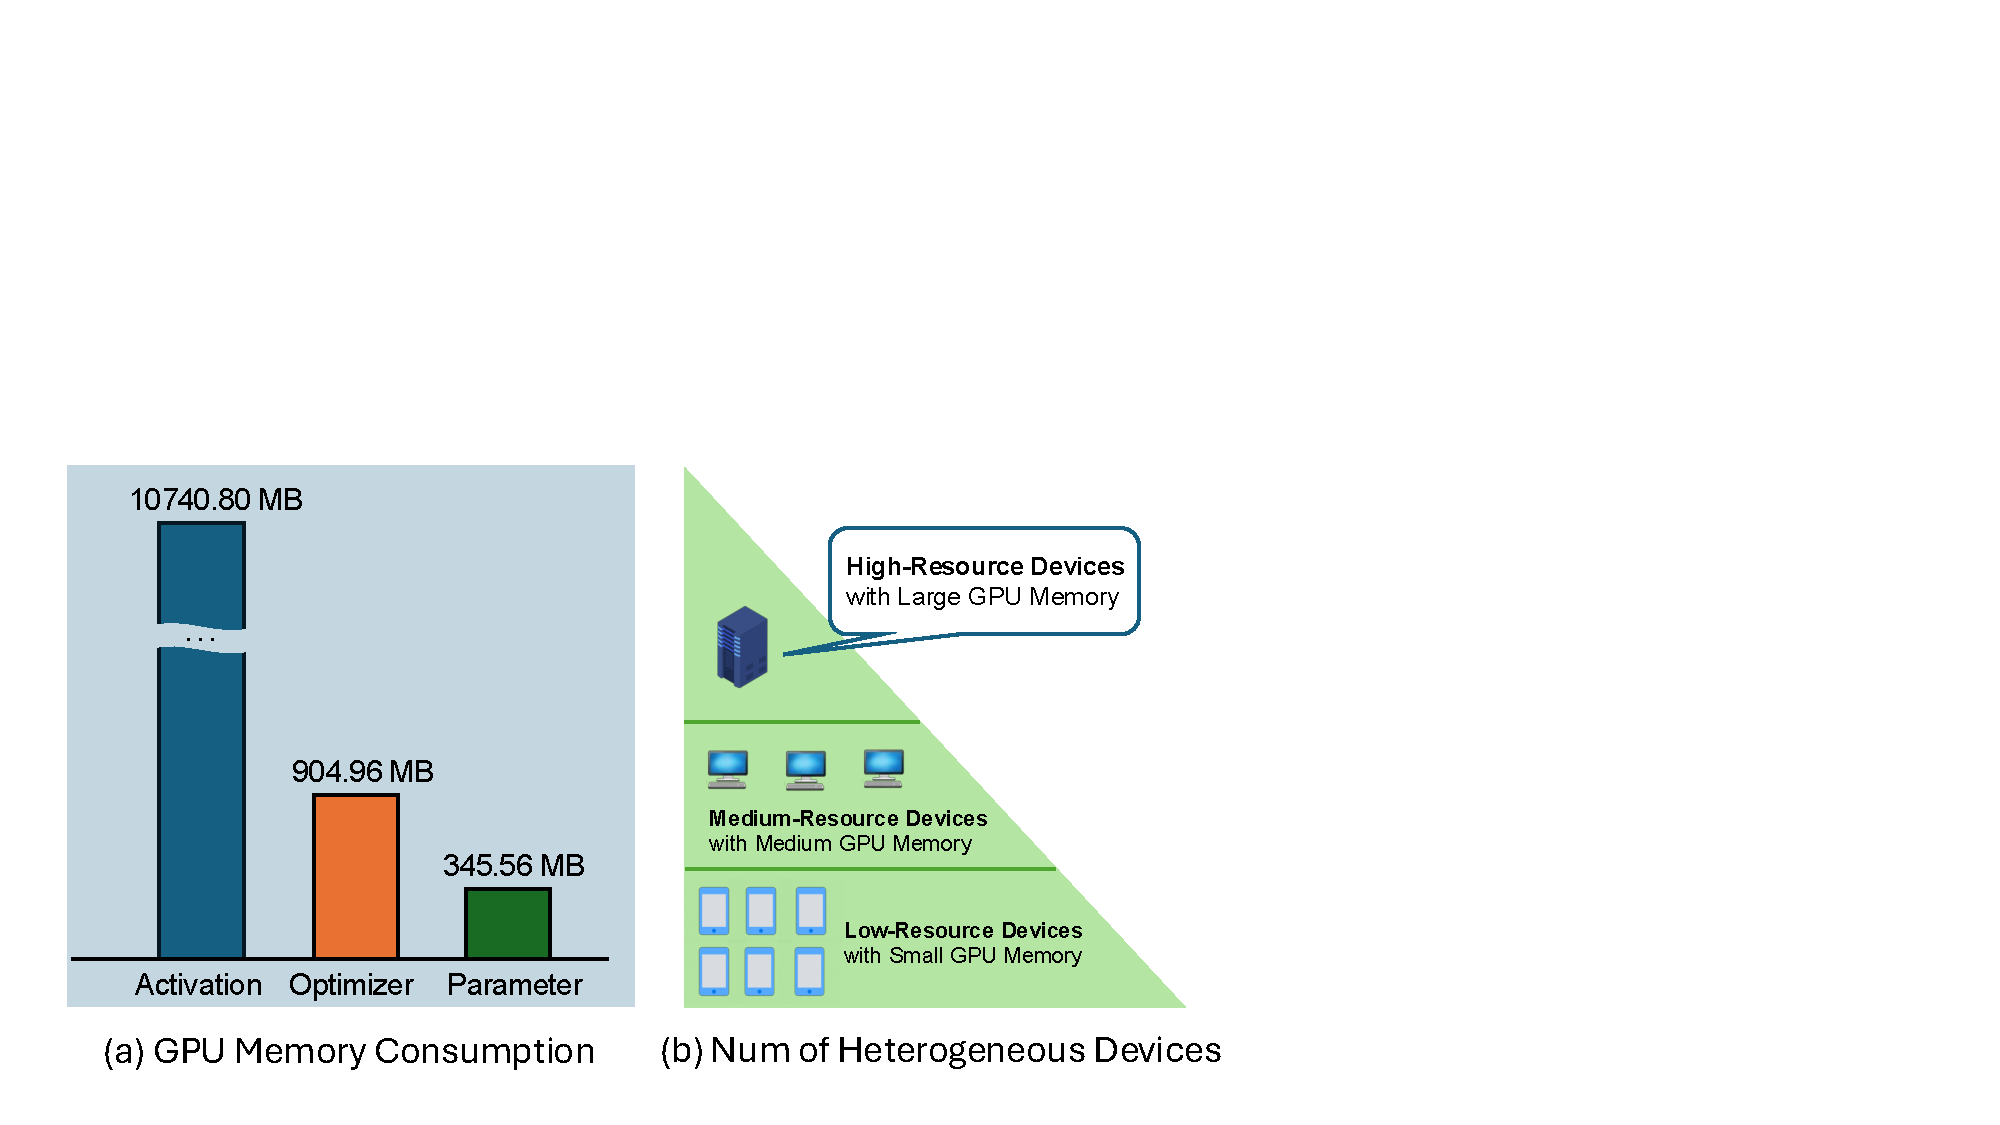
\includegraphics[width=0.45\textwidth]{figure/motivation-memory-latency-numClients.pdf}
% \vspace{-10pt}
\caption{(a) GPU memory usage for the ViT-base model, which includes a 12-layer encoder with LoRA applied to each layer. Batch size is 128.
(b) The distribution of heterogeneous devices in a practical scenario.
}
\label{fig:motivation}
% \vspace{-100pt} 
\end{figure}

%%%%%%%%%%%%%%%%%%%%%%%%%%%%%%%%%%%%%%%%%%%%%%%%%%%
\section{Related Works}\label{sec:relatedwork}

\textbf{Parameter-efficient fine-tuning.} 
% Numerous trainable parameters limit resource-constrained devices from training a FM from scratch or full-tuning it for complex machine learning tasks. 
Resource-constrained devices cannot train an FM from scratch or fully fine-tune an FM due to the numerous trainable parameters.
Consequently, researchers have turned to {PEFT} techniques~\cite{ding2022delta, lester2021power, zaken2022bitfit, hu2021lora}, which involve updating only a small subset of the model's parameters. It can be mainly categorized into two types: additive and selective PEFT methods. Additive PEFT methods introduce new trainable layers to the model while keeping the pre-trained model weights frozen, enabling efficient task-specific fine-tuning. For example, prompt tuning~\cite{lester2021power} adds task-specific soft prompts, which are then fine-tuned to adapt the model to new tasks. 
% Prefix tuning~\cite{li2021prefix} extends trainable soft prompts to each input of transformer layers to further enhance feature modeling {capabilities}. 
% LoRA~\cite{hu2021lora} constrains the update of a pre-trained weight matrix by decomposing it into a product of two smaller matrices, which are then trained. 
LoRA~\cite{hu2021lora} introduces trainable low-rank matrices that are added to the existing weights of the pre-trained model for fine-tuning. 
% 
Selective PEFT methods update only a subset of the pre-trained model's parameters. For instance, BitFit~\cite{zaken2022bitfit} updates only the bias parameters, while LN-Norm~\cite{basu2024strong} updates the layer normalization parameters in ViT models. Further advancements have been made with hybrid approaches that combine multiple PEFT techniques to enhance fine-tuning efficiency~\cite{he2021towards, zhou2023autopeft}. Among these PEFT methods, LoRA has demonstrated more stable and effective performance for complex downstream tasks with mid-size datasets~\cite{ding2022delta, zhang2023fedpetuning}. Without loss of generality, we focus on LoRA in this work. 

% This approach allows for effective adaptation to new tasks without the need for extensive computational resources.
% As such, researchers~\cite{ding2022delta, lester2021power, zaken2022bitfit, hu2021lora} turn to fine-tuning by updating only a small set of model parameters, known as parameter-efficient fine-tuning. 
% There are three categories of PEFT, including additive methods, selective methods, and re-parameterization-based methods. Additive methods add new trainable layers to the model \ping{while} keep the \ping{initial} model weights frozen, \ping{allowing for efficient task-specific fine-tuning}.
% and updating only the new layer weights. This approach efficiently fine-tunes the foundation models for specific tasks. 
% Prompt Tuning~\cite{lester2021power} adds task-specific soft prompts \ping{that are fine-tuned to adapt the model to new tasks}.
% and fine-tuning those soft prompts to adapt to new tasks. 
% Prefix Tuning~\cite{li2021prefix} extends trainable soft prompts to each input of transformer layers to further enhance feature modeling \ping{capabilities}. 
% Adapter~\cite{houlsby2019parameter} instead adds \ping{small} trainable layers inside each transformer layer for fine-tuning purposes. 
% Selective-based methods involve updating only a few selected foundation model layers. BitFit~\cite{zaken2022bitfit} only updates bias parameters, while LN-Norm~\cite{basu2024strong} updates layer norm in ViT-based models.
% % while Diff Pruning~\cite{guo2021parameter} creates task-specific difference vectors and updates them. 
% Re-parameterization-based methods decompose a weight matrix into lower-rank matrices, as seen in LoRA~\cite{hu2021lora}. 

% \ping{Further advancements have been made with hybrid approaches} ~\cite{he2021towards, zhou2023autopeft} that \ping{combine multiple PEFT techniques to enhance fine-tuning efficiency}.
% % use multiple PEFT technologies to further improve fine-tuning abilities. 
% % However, additive-based and selective-based methods result in unfavorable performance, while re-parameterization-based methods offer much more stable performance. 
% Among these PEFT methods, LoRA have demonstrated more stable and effective performance~\cite{ding2022delta, zhang2023fedpetuning}. Without loss of generality, we consider LoRA in this work. 

{\textbf{Federated LoRA-based fine-tuning.} 
Given the resource challenges posed by full-model fine-tuning~\cite{li2023fedtp} in FL, federated LoRA-based fine-tuning has gained increasing attention~\cite{liu2023differentially,zhang2023towards,babakniya2023slora,wu2024fedfmsl,wu2024fedbiot,sun2024improving,gao2025flowertune}. These approaches improve the parameter efficiency and reduce computational and communication costs~\cite{yu2023federated, zhuang2023foundation}.
% enable collaborative fine-tuning of LoRA layers across multiple clients in a FL manner~\cite{yu2023federated, zhuang2023foundation}. 
% Given the resource challenges posed by full-model fine-tuning~\cite{li2023fedtp} in FL, there is an increasing focus on federated PEFT methods~\cite{liu2023differentially,zhang2023towards,babakniya2023slora,wu2024fedfmsl,wu2024fedbiot,sun2024improving}. 
%
% PromptFL~\cite{guo2023promptfl} allows federated participants to train prompts instead of a shared model, enabling efficient global aggregation and local training, which leveraging the capabilities of FMs in a distributed manner. FedAdapter~\cite{cai2022fedadapter} integrates adapters into federated large language model fine-tuning and gradually refines the adapter configuration during training. However, LoRA-based federated fine-tuning approaches are gaining attention, as they are known to be particularly effective in mid-sized data scenarios~\cite{hu2021lora}. Several works combine LoRA-based fine-tuning with FL. 
%
For example, FedIT~\cite{zhang2023towards} proposes a vanilla federated fine-tuning method with LoRA and establishes benchmarks for PEFT in FL.
SLoRA~\cite{babakniya2023slora} designs a two-stage fine-tuning method that combines full model and LoRA-based fine-tuning to establish a better initialization for LoRA weights and improve the global model accuracy. 
FedFMSL~\cite{wu2024fedfmsl} proposes a two-stage LoRA fine-tuning framework. In the first stage, all LoRA layers are trainable to quickly adapt to the current task. In the second stage, the model is initialized with the weights obtained from the first stage, and a Sparsely Activated LoRA (SAL) algorithm is introduced to progressively activate LoRA layers for saving computational costs.
FedBiOT~\cite{wu2024fedbiot} proposes a federated LoRA-based fine-tuning algorithm that uses compressed pre-trained weights (named as emulator) on each client. By using an emulator that simulates the behavior of the original FMs on client, the computational cost for local training can be reduced.
DP-LoRA~\cite{liu2023differentially} is a vanilla approach that incorporates a Gaussian-based differential privacy (DP) mechanism into federated LoRA-based fine-tuning. By adding noise to model updates, it protects clients' privacy during the FL process.
FFA-LoRA~\cite{sun2024improving} introduces a LoRA layer initialization strategy to improve model accuracy and communication efficiency. By default, the LoRA weight matrix $A$ (input projection) is initialized with small random values, and matrix $B$ (output projection) is initialized as zero. They prove that fine-tuning only matrix $B$ is sufficient for efficient model fine-tuning.
However, these approaches often fail to account for the heterogeneity in clients' resources.}
% The most related works~\cite{cho2023heterogeneous,wang2024flora,bai2024flexlora,su2023fedra} tailor LoRA configurations for clients with different computational capabilities but face challenges in balancing computational efficiency and accuracy. We argue that an effective design of heterogeneous fine-tuning allocation is crucial for optimizing the performance of federated LoRA-based fine-tuning in resource-constrained settings.}

% % Works like FedPrompt~\cite{zhao2023fedprompt}, PromptFL~\cite{guo2023promptfl}, pFedPrompt~\cite{guo2023pfedprompt}, FedPepTAO~\cite{che2023federated}, FedTPG~\cite{qiu2024text}, MultilingualBorders~\cite{zhao2023breaking}, DiPrompT~\cite{bai2024diprompt}, FedOTP~\cite{li2024global} and FedSP~\cite{dong2023tunable}
% utilizes prompt tuning to reduce communication costs between clients and servers. FedAdapter~\cite{cai2022fedadapter} integrates adapters into federated large language fine-tuning. 
% Although these works demonstrate simplicity, they result in suboptimal performance. Another group of works employ the re-parameterization-based method (e.g., LoRA~\cite{hu2021lora}) as the PEFT method for Federated FMs fine-tuning. For example, 
% % FedPETuning~\cite{zhang2023fedpetuning} investigate the performance of federated fine-tuning language models with LoRA. 
% FedIT~\cite{zhang2023towards} employs LoRA to fine-tuning large language models for collaborative multiple-task learning. SLoRA~\cite{babakniya2023slora} designs an initialization method for LoRA-based fine-tuning. FFA-LoRA~\cite{sun2024improving} enhances the security of LoRA-based FFM with differential privacy. 
% \ping{However, these approaches frequently overlook the variability in client resources, a gap partially addressed by HETLoRA~\cite{cho2023heterogeneous} and FedRA~\cite{su2023fedra}, which attempt to tailor LoRA layers for diverse client resources but face challenges in balancing computational efficiency and accuracy}.
% % However, the aforementioned methods fail to consider heterogeneous clients with varying computational resources, rendering them inapplicable to real-world settings. HETLoRA~\cite{cho2023heterogeneous} explores on-device foundation models with diverse client resource levels through the use of different numbers of ranks for LoRA layers, but it falls short in significantly reducing computational costs and is susceptible to lower accuracy. FedRA~\cite{su2023fedra} attempts to address the heterogeneous client issue through random layer allocation. 
% We argue that \ping{an effective} design of heterogeneous layer allocation is crucial for performance optimization.

{\textbf{FL with heterogeneous clients.}
To address the heterogeneous resource capabilities of clients in FL, existing methods~\cite{diao2020heterofl,horvath2021fjord,kim2022depthfl,liu2022no} can be broadly categorized into two types: width-wise scaling and depth-wise scaling. Width-wise scaling approaches~\cite{diao2020heterofl, horvath2021fjord} prune model channels to create a smaller and more streamlined local model for clients with limited resources to update. Depth-wise scaling approaches~\cite{kim2022depthfl, liu2022no} assign only the first few layers of the model for resource-limited clients to update, thus reducing resource requirements for clients. However, these approaches focus on full-model training and cannot be directly applied to LoRA-based fine-tuning.
There are several existing works~\cite{cho2023heterogeneous,wang2024flora,bai2024flexlora,su2023fedra,zhang2024fed} in federated LoRA-based fine-tuning consider clients with heterogeneous resources. 
HETLoRA~\cite{cho2023heterogeneous} employs a heterogeneous LoRA rank strategy, allowing clients to train different numbers of LoRA ranks based on their memory capacity, with a hierarchical aggregation rule where shared ranks are averaged across multiple clients, while higher ranks are aggregated among fewer clients.
FLoRA~\cite{wang2024flora} is designed to mitigate aggregation noise during federated LoRA-based fine-tuning. It introduces a stacking strategy for aggregation, where LoRA layer updates from clients are stacked along the rank dimension respectively, and then used to reconstruct the full weight matrices. For each next round, the LoRA layers are initialized on each clients and only the full weight matrices are updated.
FlexLoRA~\cite{bai2024flexlora} introduces a novel aggregation strategy that first aggregates LoRA weight matrices $A$ and $B$ separately. Then those aggregated LoRA weights are used to reconstruct the full weight matrices for each LoRA layer. Finally, they 
apply singular value decomposition (SVD) to redistribute the LoRA weight matrices among clients with varying ranks.
% However, these rank-based methods reducing the LoRA rank alone does not lead to substantial memory savings, making it less effective for memory-constrained environments, not alone the FlexLoRA involves more computational cost by using the SVD algorithm.
However, reducing LoRA ranks in these rank-based methods can only reduce the memory cost of optimizer states, making them less effective in memory-constrained environments.
FedRA~\cite{su2023fedra} introduces a layer-wise LoRA allocation strategy that randomly selects partial LoRA layers in each round to address resource constraints among clients. However, this method overlooks the varying importance of different layers in the global model’s accuracy.}
% Another challenge in FL is the non-IID nature of the client dataset, which can substantially affect training accuracy due to variations in data quantities, labels, and domains~\cite{mcmahan2017communication, li2022federated}. We recognize that simplistic datasets fail to accurately evaluate the performance of federated fine-tuning~\cite{charles2024towards, ye2024openfedllm}. Therefore, in this work, we design three comprehensive benchmark datasets that simulate various settings of data and resource heterogeneity. These benchmarks provide a more realistic assessment of the challenges and performance of federated fine-tuning in diverse and heterogeneous environments.

{In Table~\ref{tab:survey}, we provide an overall comparison of our approach with the state-of-the-art (SOTA) methods discussed above. By evaluating four key aspects: whether to use PEFT techniques, whether to consider resource and model heterogeneity, and whether incorporating a dynamic training strategy based on training-time model performance. Overall, our method demonstrates clear advantages over existing works.}

\begin{table}[htbp]
% \color{NavyBlue}
  % \arrayrulecolor{NavyBlue}
  \centering
  \caption{{Compared with SOTA Works.}}
  \scalebox{0.80}{
    \begin{tabular}{ccccccccc}
    \toprule[2pt]
    \textbf{{Method}}   & \textbf{{PEFT}} & \textbf{{Resource Hete.}} & \textbf{{Model Hete.}} & \textbf{{Dynamic Training}}  \\
    \midrule
    {FedTP~\cite{li2023fedtp}}                         & {\ding{55}}        &{\ding{55}}         &{\ding{55}}         &{\ding{51}}                  \\
    % {PromptFL~\cite{guo2023promptfl}}                         & {\ding{51}}        &{\ding{55}}         &{\ding{55}}         &{\ding{55}}                  \\
    % {FedAdapter~\cite{cai2022fedadapter}}                         & {\ding{51}}        &{\ding{55}}         &{\ding{55}}         &{\ding{51}}                  \\
    {FedIT~\cite{zhang2023towards}}               & {\ding{51}}        & {\ding{55}}        & {\ding{55}}         & {\ding{55}}                   \\
    {SLoRA~\cite{babakniya2023slora}}                      & {\ding{51}}        & {\ding{55}}        & {\ding{55}}        &  {\ding{55}}                \\
    {FedFMSL~\cite{wu2024fedfmsl}}                      &{\ding{51}}         & {\ding{55}}        & {\ding{55}}        &  {\ding{51}}                 \\
    % {FwdLLM~\cite{xu2024fwdllm}}                     & {\ding{51}}        & {\ding{55}}        & {\ding{55}}        & {\ding{55}}                  \\
    {FedBiOT~\cite{wu2024fedbiot}}                     &{\ding{51}}         & {\ding{55}}        &{\ding{55}}         & {\ding{51}}                 \\
    {DP-LoRA~\cite{liu2023differentially}}                      & {\ding{51}}        & {\ding{55}}        & {\ding{55}}        & {\ding{55}}                \\
    {FFA-LoRA~\cite{sun2024improving}}                      & {\ding{51}}        & {\ding{55}}        & {\ding{55}}        & {\ding{55}}                  \\
    % {FedKSeed~\cite{fedkseed2024}}                          &{\ding{55}}         & {\ding{55}}        & {\ding{55}}        & {\ding{51}}                  \\
    {FLoRA~\cite{wang2024flora}}                          & {\ding{51}}        & {\ding{51}}        & {\ding{51}}        & {\ding{55}}               \\
    {FlexLoRA~\cite{bai2024flexlora}}                         & {\ding{51}}        & {\ding{51}}        & {\ding{51}}        & {\ding{55}}               \\
    % {FEDLPP~\cite{jianhao2024promoting}}            &{EMNLP}         &         &         &         &                  \\
    {HETLoRA~\cite{cho2023heterogeneous}}                   & {\ding{51}}        & {\ding{51}}        & {\ding{51}}        &  {\ding{55}}              \\
    {FedRA~\cite{su2023fedra}}                          &{\ding{51}}         & {\ding{51}}        & {\ding{51}}        & {\ding{55}}                 \\
    \midrule
    \textbf{{Ours}}                   & {\ding{51}} & {\ding{51}} & {\ding{51}} & {\ding{51}}  \\
    \bottomrule[2pt]
    \end{tabular}%
    }
  \label{tab:survey}%
  \arrayrulecolor{black}
\end{table}%


% \begin{table*}[htbp]
% \arrayrulecolor{NavyBlue}
%   \centering
%   \caption{{Compared with State-of-the-art Works.}}
%   \scalebox{0.95}{
%     \begin{tabular}{ccccccccc}
%     \toprule[2pt]
%     \textbf{{Method}} & \textbf{{Year}} & \textbf{{Publisher}} & \textbf{{PEFT}} & \textbf{{Resource Hete.}} & \textbf{{Model Hete.}} & \textbf{{Dynamic Training}} & \textbf{{Miscellaneous Data}} & \textbf{{Large FMs}} \\
%     \midrule
%     {FedTP~\cite{li2023fedtp}}     & {2023}           &{TNNLS}         & {\ding{55}}        &{\ding{55}}         &{\ding{55}}         &{\ding{51}} &{\ding{55}} &{\ding{55}}                  \\
%     {DP-LoRA~\cite{liu2023differentially}}     & {2023}           &{TMIS}         & {\ding{51}}        & {\ding{55}}        & {\ding{55}}        & {\ding{55}} &{\ding{51}}  &{\ding{51}}               \\
%     {FedIT~\cite{zhang2023towards}}       & {2023}           &{NeurIPSW}         & {\ding{51}}        & {\ding{55}}        & {\ding{55}}         & {\ding{55}}  &  {\ding{55}}    & {\ding{51}}                  \\
%     {SLoRA~\cite{babakniya2023slora}}     & {2023}           &{NeurIPSW}         & {\ding{51}}        & {\ding{55}}        & {\ding{55}}        &  {\ding{55}} & {\ding{55}} & {\ding{55}}                \\
%     {FedMS~\cite{wu2024fedfmsl}}    & {2024}           &{TMC}         &{\ding{51}}         & {\ding{55}}        & {\ding{55}}        &  {\ding{51}} &{\ding{51}} & {\ding{55}}                \\
%     {FwdLLM~\cite{xu2024fwdllm}}    & {2024}           &{USENIX ATC}        & {\ding{51}}        & {\ding{55}}        & {\ding{55}}        & {\ding{55}} &{\ding{51}} & {\ding{55}}                 \\
%     {FedBiOT~\cite{wu2024fedbiot}}    & {2024}           &{KDD}         &{\ding{51}}         & {\ding{55}}        &{\ding{55}}         & {\ding{51}} & {\ding{51}} & {\ding{51}}                 \\
%     {FFA-LoRA~\cite{sun2024improving}}    & {2024}           &{ICLR}         & {\ding{51}}        & {\ding{55}}        & {\ding{55}}        & {\ding{55}} & {\ding{51}} & {\ding{51}}                 \\
%     {FedKSeed~\cite{fedkseed2024}}        & {2024}           &{ICML}         &{\ding{55}}         & {\ding{55}}        & {\ding{55}}        & {\ding{51}} &{\ding{51}} & {\ding{51}}                 \\
%     {FLoRA~\cite{wang2024flora}}        & {2024}           &{NeurIPS}         & {\ding{51}}        & {\ding{51}}        & {\ding{51}}        & {\ding{55}}    & {\ding{51}} & {\ding{51}}             \\
%     {FlexLoRA~\cite{bai2024flexlora}}        & {2024}           &{NeurIPS}         & {\ding{51}}        & {\ding{51}}        & {\ding{51}}        & {\ding{55}}   &{\ding{51}} &{\ding{51}}              \\
%     % {FEDLPP~\cite{jianhao2024promoting}}    & {2024}           &{EMNLP}         &         &         &         &                  \\
%     {HETLoRA~\cite{cho2023heterogeneous}} & {2024}           &{EMNLP}         & {\ding{51}}        & {\ding{51}}        & {\ding{51}}        &  {\ding{55}} &{\ding{51}}  &{\ding{51}}             \\
%     {FedRA~\cite{su2023fedra}}        & {2024}           &{ECCV}         &{\ding{51}}         & {\ding{51}}        & {\ding{51}}        & {\ding{55}} &{\ding{51}} & {\ding{55}}                 \\
%     \midrule
%     \textbf{{Ours}}                       & {-}              & {-} & {\ding{51}} & {\ding{51}} & {\ding{51}} & {\ding{51}} & {\ding{51}} &{\ding{51}}  \\
%     \bottomrule[2pt]
%     \end{tabular}%
%     }
%   \label{tab:survey}%
%   \arrayrulecolor{black}
% \end{table*}%

% the diversity in data distribution among the participating parties, \ping{characterized by Non-IID data ~\cite{mcmahan2017communication} .
% % i.e., Non-IID~\cite{mcmahan2017communication}. 
% % As a result of variations in Non-IID data quantities, labels, and domains~\cite{li2022federated}, numerous distributed training endeavors for deep neural networks experience substantial losses in accuracy. 

% we argue that when it comes to foundation models, some unrealistic simple datasets and tasks will not be able to evaluate the actual performance of FFMs. Based on that, we design \hl{three} comprehensive benchmarks with multiple skews and orchestrate the design of FFMs under the challenges from both heterogeneous clients and Non-IID data.


%%%%%%%%%%%%%%%%%%%%%%%%%%%%%%%%%%%%%%%%%%%%%%%%%%%
% \section{Preliminaries}
% % \textbf{Vanilla FL System with FedAvg.}\label{sec:og-fl}
% % In a typical FL system, 
% % $n$ clients collaboratively train a global model \(\boldsymbol{\mathcal{\theta}}\) by solving the optimization problem $\min_{\boldsymbol{\mathcal{\theta}}} \mathcal{L}(\boldsymbol{\mathcal{\theta}}) := \frac{1}{n}\sum_{i=1}^{n} \mathcal{L}_{i}(\boldsymbol{\mathcal{\theta}})$ distributedly under the coordination of a central server, where $\mathcal{L}_{i}(\boldsymbol{\mathcal{\theta}})$ is the local learning objective function for client $i$. More precisely, in each training round $t$, the server randomly selects a subset \(\mathcal{S}^t\) of \(s\) clients and broadcasts the current global model \(\boldsymbol{\mathcal{\theta}}^t\) to them. 
% % Each selected client \(i \in \mathcal{S}^t\) updates the  model using its local dataset to obtain \(\boldsymbol{\mathcal{\theta}}_i^{t+1}\), and computes the local update \(\boldsymbol{\delta}_i^{t+1} := \boldsymbol{\mathcal{\theta}}_i^{t+1} - \boldsymbol{\mathcal{\theta}}^t\), which is subsequently sent to the server.
% % In Federated Averaging (FedAvg)~\cite{mcmahan2017communication}, the server aggregates these updates by \(\boldsymbol{\mathcal{\theta}}^{t+1} := \boldsymbol{\mathcal{\theta}}^t + ({1}/{|\mathcal{S}^t|})\sum_{i \in \mathcal{S}^t} \boldsymbol{\delta}_i^{t+1}\). 
% % This process iteratively improves the global model while ensuring data privacy, as raw data remains on the clients' devices.
% %%%%%%%%%%%%%%%%%%%%%%%%%%%%%%%%%%%%%%%%
% % Typically, a FL system involves a set of $n$ clients to collaboratively train a global model $\boldsymbol{\mathcal{\theta}}$ by solving the following optimization problem in a distributed and iterative manner,
% % \begin{align}\label{fed_obj}
% % \min_{\boldsymbol{\mathcal{\theta}}} \mathcal{L}(\boldsymbol{\mathcal{\theta}}) 
% %  := \frac{1}{n}\sum_{i=1}^{n} \mathcal{L}_{i}(\boldsymbol{\mathcal{\theta}})
% % \end{align}
% % where $\mathcal{L}_{i}(\boldsymbol{\mathcal{\theta}})$ represent the local learning objective function of client $i$. Specifically, in each training round $t$, the central server randomly selects a subset of $s$ clients, denoted by $\mathcal{S}^t$, and broadcasts them the global model $\boldsymbol{\mathcal{\theta}}^t$ it maintains. Each selected client $i\in \mathcal{S}^t$ updates the global model using its local dataset and obtains a local model $\boldsymbol{\mathcal{\theta}}_i^{t+1}$. In the classic FL method, Federated Averaging (FedAvg)~\cite{mcmahan2017communication}, the local model updates of clients, i.e., $\boldsymbol{\delta}_i^{t+1}=\boldsymbol{\mathcal{\theta}}_i^{t+1}-\boldsymbol{\mathcal{\theta}}^t$, will be collected and aggregated by the server to update the global model as follows:
% % \begin{align}\label{eq:og-fedavg}
% % \boldsymbol{\mathcal{\theta}}^{t+1} := \boldsymbol{\mathcal{\theta}}^t + \frac{1}{|\mathcal{S}^t|}\sum_{i\in \mathcal{S}^t}\boldsymbol{\delta}_i^{t+1},
% % \end{align}
% % for the next round of training. 

% \textbf{LoRA for FM Fine-Tuning.} 
% \hl{ready for reviewing}The idea of LoRA is to constrain the update of a pre-trained weight matrix $\boldsymbol{W}^0 \in \mathbb{R}^{d \times k}$ by a low rank decomposition $\boldsymbol{W}^0 + \Delta \boldsymbol{W} = \boldsymbol{W}^0 + \boldsymbol{B} \boldsymbol{A}$, where $\boldsymbol{B} \in \mathbb{R}^{d \times r}$, $\boldsymbol{A} \in \mathbb{R}^{r \times k}$, and the rank $r \ll \min(d, k)$. During training, $\boldsymbol{W}^0$ is frozen, and only $\boldsymbol{A}$ and $\boldsymbol{B}$ are updated. We consider a pre-trained model $\boldsymbol{\Phi}^0 = \{\boldsymbol{W}_{(1)}^0, \cdots, \boldsymbol{W}_{(l)}^0, \boldsymbol{W}_{rest}^0\}$ with $l$ transformer layers, where each transformer layer is $\boldsymbol{W}_{(j)}^0$ with $j \in [1, l]$, and $\boldsymbol{W}_{rest}^0$ represents the the remaining layers. LoRA is typically applied to specific modules within transformer layers, such as the attention weights~\cite{hu2021lora}. 
% We denote the LoRA layer added to the $j$-th transformer layer as $\Delta\boldsymbol{{W}}_{(j)}$ and any additional trainable parameters in the embedding or classifier layers as $\Delta\boldsymbol{W}_{rest}$. 
% \ping{In this work, we emphasize LoRA's application to attention weights within transformer layers, which are computationally intensive, thereby optimizing performance and efficiency. For clarity, we define the set of trainable parameters as \(\boldsymbol{\mathcal{\theta}}:= \{\Delta\boldsymbol{W}_{(1)}, \cdots, \Delta\boldsymbol{W}_{(l)}\}\), simplifying the model by omitting \(\Delta\boldsymbol{W}_{rest}\).}

% % This work focuses on LoRA layers due to their significant proportion of trainable parameters and memory usage. In practice, LoRA is applied to multiple specific modules or weight matrices (usually the attention weights) within each transformer layer~\cite{hu2021lora}, which is often the most computationally intensive part of the model. Here, we use $\Delta\boldsymbol{{W}}_{(j)}$ to represent the LoRA layer added to the $j$-th transformer layer $\boldsymbol{W}_{(j)}^0$, and use $\Delta\boldsymbol{W}_{rest}$ to represent the remaining possible trainable parameters in the embedding or classifier layers. We focus on the design of LoRA layers because of their significant proportion of trainable parameters and memory usage. For simplicity, we omit  $\Delta\boldsymbol{W}_{rest}$ and define the trainable parameters as $\boldsymbol{\mathcal{\theta}}:= \{\Delta\boldsymbol{{W}}_{(1)}, \cdots, \Delta\boldsymbol{{W}}_{(l)}\}$. 


% % \subsection{LoRA for Foundation Model Fine-Tuning.} \label{sec:og-lora}
% % Low-rank adaption, known as LoRA~\cite{hu2021lora}, stands out as a promising fine-tuning technique for foundation models~\cite{kuang2023federatedscope}. In this work, we consider a pre-trained model $\boldsymbol{\Phi}^0$ with $l$ transformer layers, where each transformer layer is denoted as $\boldsymbol{W}_{(j)}^0$ with $j \in [1, l]$, and the remaining layers of the model are denoted as $\boldsymbol{W}_{rest}^0$. Thus, the pre-trained model is represented as $\boldsymbol{\Phi}^0 = \{\boldsymbol{W}_{(1)}^0, \cdots, \boldsymbol{W}_{(l)}^0, \boldsymbol{W}_{rest}^0\}$. Unlike full-model fine-tuning where the trainable parameters $\boldsymbol{\mathcal{\theta}}$ have the same dimension as the pre-trained weights (i.e., $\dim(\boldsymbol{\mathcal{\theta}})=\dim(\boldsymbol{\Phi}^0)$), LoRA is more parameter-efficient with $\dim(\boldsymbol{\mathcal{\theta}})\ll\dim(\boldsymbol{\Phi}^0)$. The core idea of LoRA is to constrain the update of a pre-trained weight matrix $\boldsymbol{W}^0 \in \mathbb{R}^{d \times k}$ by a low rank decomposition $\boldsymbol{W}^0 + \Delta \boldsymbol{W} = \boldsymbol{W}^0 + \boldsymbol{B} \boldsymbol{A}$, where $\boldsymbol{B} \in \mathbb{R}^{d \times r}$, $\boldsymbol{A} \in \mathbb{R}^{r \times k}$, and the rank $r \ll \min(d, k)$. During training, $\boldsymbol{W}^0$ is frozen, while $\boldsymbol{A}$ and $\boldsymbol{B}$ are trainable. 
% % % % The core idea of LoRA is that a pre-trained foundation model with low ``instrisic dimension'' trainable parameters can still efficiently adapt to a new task. 
% % % % For a pre-trained weight matrix $\boldsymbol{W}_0 \in \mathbb{R}^{d \times k}$, we update it using a low-rank decomposition $\boldsymbol{W}_0 + \Delta \boldsymbol{W} = \boldsymbol{W}_0 + \boldsymbol{B} \boldsymbol{A}$, where $\boldsymbol{B} \in \mathbb{R}^{d \times r}$ and $\boldsymbol{A} \in \mathbb{R}^{r \times k}$, with $r \ll \min(d, k)$. During training, $\boldsymbol{W}_0$ is fixed, while $\boldsymbol{A}$ and $\boldsymbol{B}$ are trainable. Both $\boldsymbol{W}_0$ and $\Delta \boldsymbol{W}$ are multiplied by the same input, and their outputs are summed. For $\boldsymbol{h} = \boldsymbol{W}_0 \boldsymbol{x}$, the modified forward pass is:
% % % \[
% % % % \boldsymbol{h} = \boldsymbol{W}_0 \boldsymbol{x} + \Delta \boldsymbol{W} \boldsymbol{x} = \boldsymbol{W}_0 \boldsymbol{x} + \boldsymbol{B} \boldsymbol{A} \boldsymbol{x}
% % % \] 
% % In practice, LoRA is applied to multiple specific modules or weight matrices (usually the attention weights) within each transformer layer~\cite{hu2021lora}. Here, we use $\Delta\boldsymbol{{W}}_{(j)}$ to represent the LoRA layer added to the $j$-th transformer layer $\boldsymbol{W}_{(j)}^0$,
% % % which we denote as $\Delta\boldsymbol{{W}}_j$. 
% % % The LoRA $\Delta\boldsymbol{{W}}_j\in\mathbb{R}^{d\times k}$ is represented with a low-rank decomposition $B_{j}A_{j}$, where $B\in\mathbb{R}^{d\times r}$, $A\in\mathbb{R}^{r\times k}$, and the parameter-efficiency is by keeping $r\ll min(d,k)$. 
% % % By doing so, the original middle feature input $x_{m}$ and middle feature output $y_{m}=\boldsymbol{W}_j^0 x_{m}$ will be modified to,
% % % \begin{equation}\label{eq:lora}
% % % y_{m}=\boldsymbol{W}_j^0 x_{m} + \Delta\boldsymbol{{W}}_j x_{m}.
% % % \end{equation}
% % % In the rest of the paper, we use $\Delta\boldsymbol{{W}}:=\{\Delta\boldsymbol{{W}}_0, \cdots, \Delta\boldsymbol{{W}}_{l-1}\} $ to represent the set of added LoRA layers.
% % and use $\Delta\boldsymbol{W}_{rest}$ to represent the remaining possible trainable parameters in the embedding or classifier layers.

% % In this work, we will focus on the design of LoRA layers because of their significant proportion of trainable parameters and memory usage. For simplicity, we omit  $\Delta\boldsymbol{W}_{rest}$ and use $\boldsymbol{\mathcal{\theta}}:= \{\Delta\boldsymbol{{W}}_{(1)}, \cdots, \Delta\boldsymbol{{W}}_{(l)}\}$ to represent the trainable LoRA parameters. 

% % % , hence, the trainable parameters can be represented as $\boldsymbol{\mathcal{\theta}}:= \{\Delta\boldsymbol{{W}}_0, \cdots, \Delta\boldsymbol{{W}}_{l-1},\Delta\boldsymbol{W}_{rest}\}$. 

% %%%%%%%%%%%%%%%%%%%%%%%%%%%%%%%%%%%%%%%%%%%%%%%%%%%
\section{Our Proposed Approach: Fed-HeLLo}
In this section, we present Fed-HeLLo, a novel framework of federated LoRA-based fine-tuning. 
Fed-HeLLo is designed for training heterogeneous LoRA layers across different clients. 
To improve the global model's performance in Fed-HeLLo, we design the HLA strategy that adaptively allocates trainable LoRA layers according to both the dynamic and intrinsic importance. 
%In Section~\ref{sec:problem-formulation}, we provide an overview of the Fed-HeLLo framework.
% by introducing the optimization problem and heterogeneous aggregation rules. We also explain the memory bottleneck issue and the varying importance of different LoRA layers, ending by summarizing the overall framework with HLA strategy
%
%In Section~\ref{sec:hla}, we design our HLA strategies in considering of intrinsic and dynamic layer importance.
% In Section~\ref{sec:GD-DPP-HLA}, we introduce GD-HLA strategies and its randomized version RGD-HLA.
% four different GD-HLA strategies that consider the intrinsic layer importance from different perspectives and present a randomized version with prior probability to enhance the robustness of HLA. 
% In Section~\ref{sec:FIM-HLA}, we discuss the dynamic layer importance and introduce FIM-HLA. 
% Finally, in Section~\ref{sec:design-framework}, we co-design GD-HLA and FIM-HLA and obtain the general HLA strategy for Fed-HeLLo.
% In Section~\ref{sec:complexity}, we analysis the computational and communication complexity.
%
% Dynamic Prior-Probability-based HLA; in Section~\ref{sec:FIM-HLA}, we introduce a Fisher Information Matrix Score-based HLA and demonstrate the entire Fed-HeLLo process by incorporating proposed HLAs.
% In this section, we introduce a novel federated FM fine-tuning method, called Fed-HeLLo, which enables clients with varying computational capabilities to heterogeneously train a local subset of LoRA layers. We then propose three different local LoRA allocation strategies to enhance the global model's fine-tuning performance. 
%
% heterogeneous local LoRA layer allocations, Fed-HLA, 
% Fed-HeLLo with various layer allocation strategies and empirically illustrate the importance of following the guidelines we proposed at beginning.



\subsection{FedHeLLo: Federated LoRA-based Fine-Tuning with Heterogeneous LoRA Allocation}\label{sec:problem-formulation} 
The idea behind LoRA is to constrain the update of a pre-trained weight matrix $\boldsymbol{W}^0 \in \mathbb{R}^{d \times k}$ by a low-rank decomposition $\boldsymbol{W}^0 + \Delta \boldsymbol{W} = \boldsymbol{W}^0 + \boldsymbol{B} \boldsymbol{A}$, where $\boldsymbol{B} \in \mathbb{R}^{d \times r}$, $\boldsymbol{A} \in \mathbb{R}^{r \times k}$, and the rank $r \ll \min(d, k)$. During training, $\boldsymbol{W}^0$ remains frozen, and only $\boldsymbol{A}$ and $\boldsymbol{B}$ are updated. We consider a pre-trained model $\boldsymbol{\Phi}^0 = \{\boldsymbol{W}_{(1)}^0, \cdots, \boldsymbol{W}_{(l)}^0, \boldsymbol{W}_{rest}^0\}$ with $l$ transformer layers, where each transformer layer is $\boldsymbol{W}_{(j)}^0$ with $j \in [1, l]$, and $\boldsymbol{W}_{rest}^0$ represents the remaining layers. LoRA is typically applied to specific modules within transformer layers, such as the attention weights~\cite{hu2021lora}. 
{We denote the LoRA layer added to the $j$-th transformer layer as 
% $\Delta\boldsymbol{{W}}_{(j)}=\{\boldsymbol{A}_{(j)}, \boldsymbol{B}_{(j)}\}$
$\boldsymbol{\theta}_{(j)} = \{\boldsymbol{A}_{(j)}, \boldsymbol{B}_{(j)}\}$
and any additional trainable parameters in the embedding or classifier layers as $\Delta\boldsymbol{W}_{rest}$.} 
% In this work, we focus on LoRA's application to attention weights within transformer layers, which are computationally intensive, thereby optimizing both performance and efficiency. 
% For simplicity, 
Here, we define the set of trainable parameters as { \(\boldsymbol{\mathcal{\theta}}:= \{\boldsymbol{\mathcal{\theta}}_{(1)}, \cdots, \boldsymbol{A}_{(l)}, \boldsymbol{B}_{(l)}\}\), simplifying the representation by omitting \(\Delta\boldsymbol{W}_{rest}\).}


We consider a federated LoRA-based fine-tuning system where $n$ clients collaboratively fine-tune a global model $\boldsymbol{\Phi}$, consisting of frozen weights $\boldsymbol{\Phi}^0$ and trainable parameters $\boldsymbol{\mathcal{\theta}}$, under the coordination of a central server. Each client $i\in [n]$ holds a local dataset $D_i\sim\mathcal{P}_i$, where $\mathcal{P}_i$ represents the data distribution specific to client $i$.
% and can vary significantly across clients. 
The problem of federated LoRA-based fine-tuning can be formulated as follows:
\begin{equation}\label{eq:ffm_obj}
\min_{\boldsymbol{\mathcal{\theta}}} \mathcal{L}(\boldsymbol{\mathcal{\theta}}) := \frac{1}{n}\sum_{i=1}^{n} \mathcal{L}_{i}(\boldsymbol{\mathcal{\theta}}; \boldsymbol{\Phi}^0),
\end{equation}
% where $\boldsymbol{\mathcal{\theta}}$ represents the trainable parameters, specifically the $l$ LoRA layers in the model when using LoRA. 
where $\mathcal{L}_{i}(\boldsymbol{\mathcal{\theta}}; \boldsymbol{\Phi}^0) := \mathbb{E}_{x \in  D_i}[\ell(\boldsymbol{\mathcal{\theta}};\boldsymbol{\Phi}^0,x)]$ denotes the local loss of client $i$, and $\ell(\boldsymbol{\mathcal{\theta}};\boldsymbol{\Phi}^0,x)$ is the loss function of the model $\boldsymbol{\Phi}=\{\boldsymbol{\mathcal{\theta}}, \boldsymbol{\Phi}^0 \}$ for a data point $x$ sampled from ${D}_i$. 
% 
% \ping{overlapped with section 3? If yes, please consider to condense the content here.} \hu{yes, overlapped, ok to remove the "Vanilla FL System with FedAvg" paragraph in section 3.}
To solve this problem, one can follow the classic FL algorithm FedAvg~\cite{mcmahan2017communication}. Specifically, before training, the server broadcasts the initial global model $\boldsymbol{\Phi}_g^0=\{\boldsymbol{\mathcal{\theta}}_g^0,\boldsymbol{\Phi}^0\}$ to all clients, where $\boldsymbol{\mathcal{\theta}}_g^0$ represents the initialized global trainable parameters. Clients then save this model as their initial local models $\boldsymbol{\Phi}_i^0, i\in[n]$. In each training round $t\in[T]$, the server sends its current global trainable parameters $\boldsymbol{\mathcal{\theta}}_g^t$ to a subset of $s$ clients, denoted by $\mathcal{S}^t$. Each selected client initializes its local trainable parameters $\boldsymbol{\mathcal{\theta}}_i^{t}$ with $\boldsymbol{\mathcal{\theta}}_g^t$ and obtains the local model $\boldsymbol{\Phi}_i^{t}= \{\boldsymbol{\mathcal{\theta}}_i^{t},\boldsymbol{\Phi}^0\}$. Based on $\boldsymbol{\Phi}_i^{t}$, the client updates $\boldsymbol{\mathcal{\theta}}_i^{t}$ individually using $D_i$ to obtain $\boldsymbol{\mathcal{\theta}}_i^{t+1}$ and sends its local update $ \boldsymbol{\delta}_i^{t+1} := \boldsymbol{\mathcal{\theta}}_i^{t+1} - \boldsymbol{\mathcal{\theta}}_i^t$ to the server. The global trainable parameters are then updated as follows:
% \begin{equation}\label{eq:og-fedavg}
$
\boldsymbol{\mathcal{\theta}}_g^{t+1} := \boldsymbol{\mathcal{\theta}}_g^t + ({1}/{|\mathcal{S}^t|})\sum_{i\in \mathcal{S}^t}\boldsymbol{\delta}_i^{t+1},
$
% \end{equation}
resulting in the global model $\boldsymbol{\Phi}_g^{t+1}=\{\boldsymbol{\mathcal{\theta}}_g^{t+1},\boldsymbol{\Phi}^0\}$ for the next round of training. 


\begin{figure}[t]
\centering
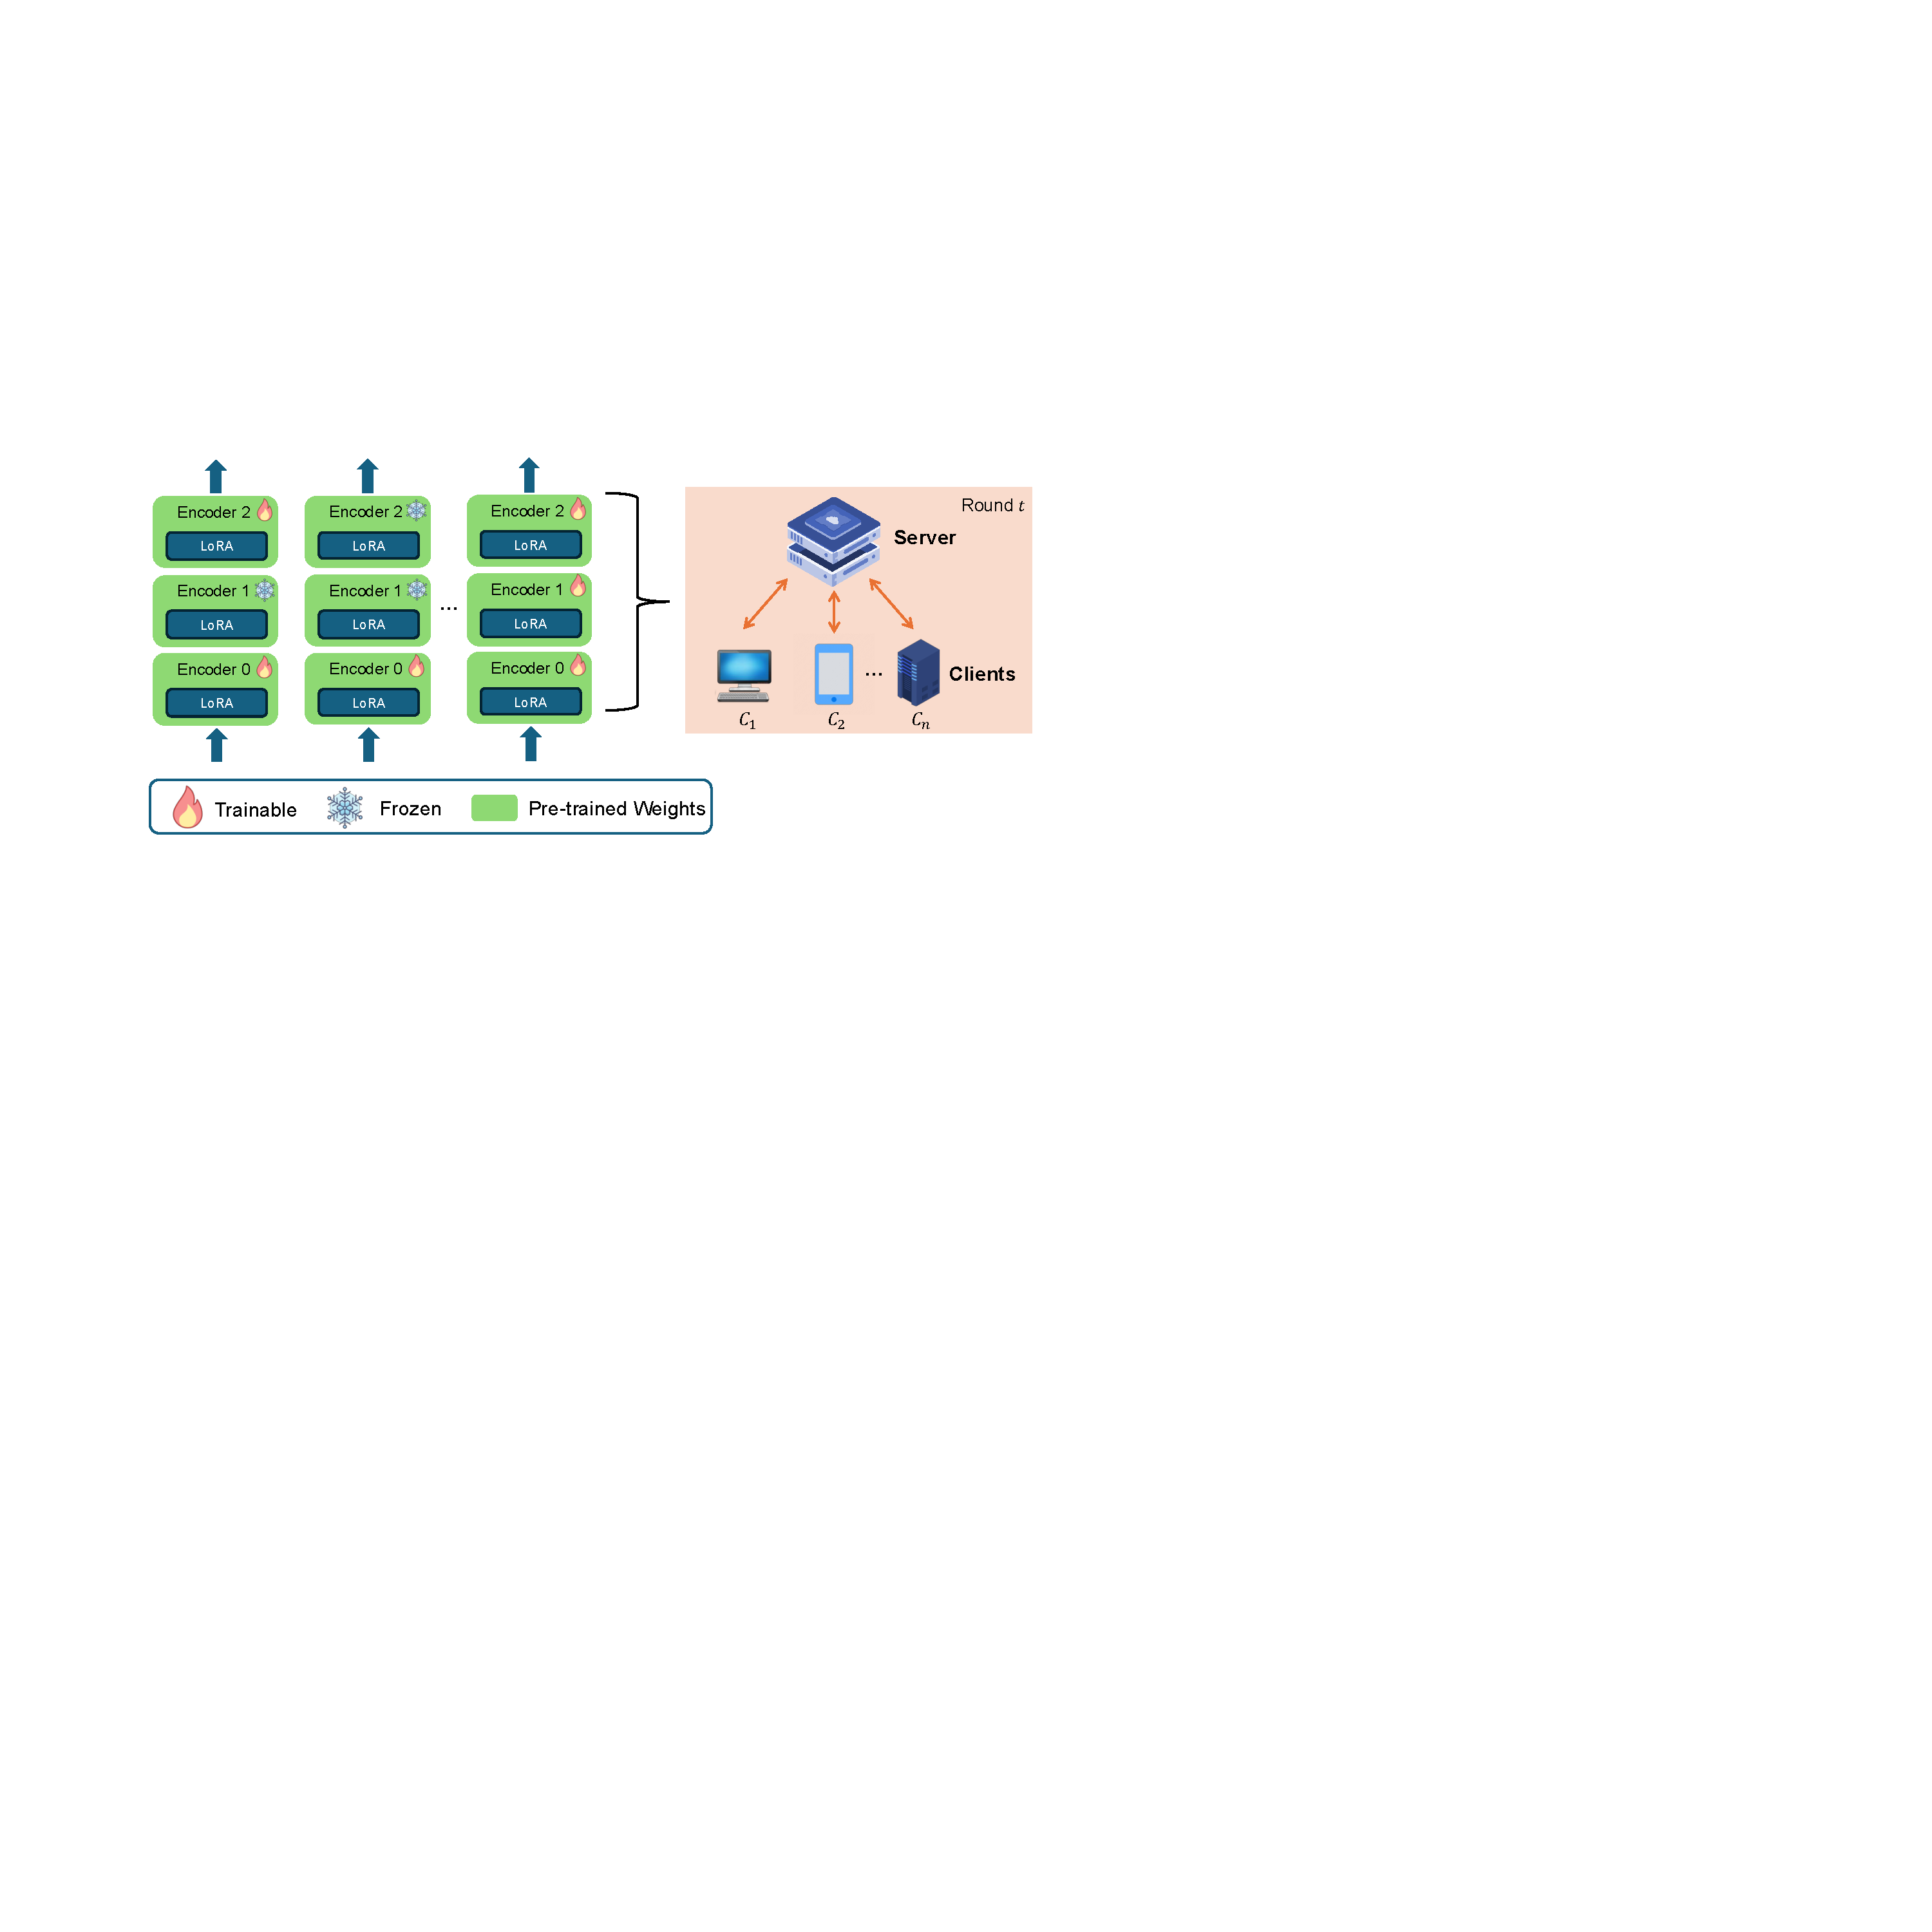
\includegraphics[width=0.50\textwidth]{figure/framework.pdf}
% \vspace{-10pt}
\caption{Overview of the Fed-HeLLo framework.
% Zoom in for a clearer view.
}
\label{fig:framework}
% \vspace{-100pt} 
\end{figure}
%%%%%%%%%%%%%%%%%%%%%%%%%%%%%%%%%%%%%%%%
% \subsection{Federated FM Fine-Tuning with Heterogeneous LoRA Allocation}
% Following Section~\ref{sec:og-fl}, we consider a typical FL system consisting of $n$ clients and a central server. These clients collaboratively fine-tune a global model $\boldsymbol{\Phi}$ containing frozen weights $\boldsymbol{\Phi}^0$ and trainable parameters $\boldsymbol{\mathcal{\theta}}$, under the coordination of the server. 

% Assuming each client $i\in [n]$ holds a local dataset $D_i\sim\mathbb{P}_i$, where the distribution $\mathbb{P}_i$ represents the unique data distribution specific to client $i$ and can vary significantly across clients. The problem of federated FM fine-tuning can be formulated as follows:
% \begin{align}\label{eq:ffm_obj}
% \min_{\boldsymbol{\mathcal{\theta}}} f(\boldsymbol{\mathcal{\theta}}) := \frac{1}{n}\sum_{i=1}^{n} f_{i}(\boldsymbol{\mathcal{\theta}}; \boldsymbol{\Phi}^0),
% \end{align}

% where $\boldsymbol{\mathcal{\theta}} =\{\Delta\boldsymbol{{W}}_{(1)}, \cdots, \Delta\boldsymbol{{W}}_{(l)}\}$ representing a set of $l$ LoRA layers; $f_{i}(\boldsymbol{\mathcal{\theta}}; \boldsymbol{\Phi}^0) := \mathbb{E}_{x \in  D_i}[\ell(\boldsymbol{\mathcal{\theta}};\boldsymbol{\Phi}^0,x)]$ represents the local loss of client $i$, and $\ell(\boldsymbol{\mathcal{\theta}};\boldsymbol{\Phi}^0,x)$ is the loss function on the global model $\boldsymbol{\Phi}=\{\boldsymbol{\mathcal{\theta}}, \boldsymbol{\Phi}^0 \}$ and datapoint $x$ sampled from ${D}_i$. 

% % \hu{revise: define global and local trainable parameters separately; define global model and local model separately } 

% % 

% Specifically, at the first round of training, the server broadcasts the initial global model $\boldsymbol{\Phi}_g^0=\{\boldsymbol{\mathcal{\theta}}_g^0,\boldsymbol{\Phi}^0\}$ to all clients where $\boldsymbol{\mathcal{\theta}}_g^0$ represents the initial trainable parameters, and clients save the model as their initial local models $\boldsymbol{\Phi}_i^0, i\in[n]$. Thereafter, at round $t$, the server sends the global trainable parameters $\boldsymbol{\mathcal{\theta}}_g^t$ to selected clients, these clients initialize their local trainable parameters $\boldsymbol{\mathcal{\theta}}_i^{t,0}$ with $\boldsymbol{\mathcal{\theta}}_g^t$ and obtain the local model $\boldsymbol{\Phi}_i^{t,0}= \{\boldsymbol{\mathcal{\theta}}_i^{t,0},\boldsymbol{\Phi}^0\} $. During local training,
% % To solve the problem in Equation~\eqref{eq:ffm_obj} distributedly over $n$ clients, the server broadcasts the global model $\boldsymbol{\Phi}$ initialized with the pre-trained weights $\boldsymbol{\Phi}^0$ to clients before the training (note that the trainable parameters $\boldsymbol{\mathcal{\theta}}$ are initialized as zeros). During the training, at round $t$, the client updates the trainable parameters $\boldsymbol{\mathcal{\theta}}^t$ locally. 
% each selected client perform $\tau$ iterations of SGD using Adam optimizer with Weight Decay
%  % Adaptive Moment Estimation with Weight Decay
% to update the trainable layers as follows:
% \begin{equation}\label{eqn:local-adam}
% \boldsymbol{\mathcal{\theta}}_i^{t,r+1} = \boldsymbol{\mathcal{\theta}}_i^{t,r} - \eta \cdot \bm{m}_i^{t,r} / (\sqrt{\bm{v}_i^{t,r}} + \epsilon), \quad \forall r = 0, \ldots, \tau - 1.
% \end{equation}
% Here, $\boldsymbol{\mathcal{\theta}}_i^{t, r}$ represents the local trainable parameters of client $i$ at local iteration $r$ 
% % which is initialized as $\boldsymbol{\mathcal{\theta}}_i^{t, 0} = \boldsymbol{\mathcal{\theta}}^{t} = \{\Delta\boldsymbol{{W}}^t,\Delta\boldsymbol{W}_{rest}^t\}$
% ; $\eta$ is the local learning rate; $\bm{m}_i^{t,r}$ and $\bm{v}_i^{t,r}$ represent the first and second moments of the local gradient $\nabla \ell(\boldsymbol{\mathcal{\theta}}_i^{t,r}; \boldsymbol{\Phi}^0, \xi_i^{t,r})$, respectively; $\epsilon$ is a small constant to prevent division by zero. The local gradient is computed over a mini-batch $\xi_i^{t,r}$ of $B$ data points sampled from $D_i$. 

% After local training, the server collects local model updates, i.e., $\boldsymbol{\delta}_i^{t+1}= \boldsymbol{\mathcal{\theta}}_i^{t, \tau} -  \boldsymbol{\mathcal{\theta}}_g^t$, and aggregates them to update the global trainable parameters as follows:

% \begin{align}\label{eq:og-fedavg}
% \boldsymbol{\mathcal{\theta}}_g^{t+1} := \boldsymbol{\mathcal{\theta}}_g^t + \frac{1}{|\mathcal{S}^t|}\sum_{i\in \mathcal{S}^t}\boldsymbol{\delta}_i^{t+1},
% \end{align}
% and obtains the global model $\boldsymbol{\Phi}_g^{t+1}=\{\boldsymbol{\mathcal{\theta}}_g^{t+1},\boldsymbol{\Phi}^0\}$ for the next round of training. 



% % to update their local models. } \hu{need to say that updated global trainable parameters is then broadcast to the clients. and clients updates its local model using this, and perform local training on these trainable parameters; probably need a figure here}

% \textbf{Memory bottleneck of federated LoRA-based fine-tuning.}
In the naive FedAvg process described above, clients should update all the trainable parameters in $\boldsymbol{\mathcal{\theta}}_g$ locally, which includes $l$ LoRA layers. This requires substantial on-device GPU memory for optimizer states and intermediate activations (as shown in Figure~\ref{fig:motivation}). For the optimizer state, it increases linearly with the size of the trainable parameters. When applying LoRA to each transformer layer, all the activation of these layers need to be stored for backpropagation, {akin} to full-model fine-tuning. 
% to store the model parameters, optimizer states, and intermediate activations.
% Although LoRA reduces the trainable parameters compared to full-model fine-tuning, it still demands substantial memory for storing activations and optimizer states during training, {akin} to full-model fine-tuning scenarios. 
% During a feed-forward pass, each layer in the FM generates activations that are stored for the subsequent backward pass, where trainable parameters are updated. 
% When LoRA is applied to every transformer layer, the memory required for these activations becomes significant.
% , surpassing the memory needed for storing model parameters and calculating gradients, as illustrated in Figure~\ref{fig:motivation}.
% Studies~\cite{smith2022using, korthikanti2023reducing} show that modern transformer models with billions of parameters can require tens of gigabytes of memory for storing activations. 
% For optimizer's memory footprint, it increases linearly with the size of the trainable parameters. 
This high memory requirement makes the local training task infeasible for clients with limited resources~\cite{zhang2023memoryadaptive}. 

% we find a good method
Inspired by the recent model freezing methods proposed in \cite{su2023fedra,ardakani2024slimfit,pan2024lisa}, freezing a model layer can eliminate the storage of its dynamic activations, significantly reducing memory requirements for local training in federated fine-tuning. 
Moreover, training partial layers reduces the storage of optimizer states.
With model freezing, resource-constrained clients can train only partial LoRA layers based on their memory capability, as shown in Figure~\ref{fig:framework}. 


% \textbf{Varying Importance of Different LoRA Layers (Centralized): check the reference talking different importance of layers in DNN}

% \textbf{Federated fine-tuning with heterogeneous local LoRA allocation.} 

% {
% Due to the consistent architecture of transformer layers in FMs~\cite{vaswani2017attention}, LoRA layers usually have the same dimensions and structures when applied uniformly (i.e., at the same positions within each transformer layer and with the same rank) across different transformer layers~\cite{hu2021lora}.
% %
% Several studies~\cite{ardakani2024slimfit,pan2024lisa} have shown that fine-tuning only a subset of LoRA layers can lower memory requirements for resource-constrained devices. }

% Specifically, training partial LoRA layers reduces the memory footprints of optimizer states and activations

% While memory usage during training involves such as activations, parameters, and the optimizer~\cite{pan2024lisa,ardakani2024slimfit}, the overall pattern and predictability remain manageable.
%
% {Consequently, we consider heterogeneous local LoRA allocation for clients with varying resources. Given the resource constraints of client $i$, the server can estimate the number of LoRA layers $c_i$ that the client can handle, which is also represents that client's capability. The server can then strategically allocate a subset of $c_i$ trainable LoRA layers to each client for local training.}

% In this case, xxx determine xxx layers, xx denoted by xxx

{In this case, we consider a heterogeneous local LoRA allocation, where the server assigns $c_i$ trainable LoRA layers for local training based on the client's capability.}
% \uline{The key challenge is to determine an effective HLA strategy for clients with varying computational capabilities, enabling effective federated LoRA-based fine-tuning under constrained resources.}
% To mitigate the memory bottleneck, we propose that resource-limited clients train only a subset of LoRA layers, tailored to their resource capacity. 
Specifically, we use an allocation map $m_i:=\{m_{i,(1)}, m_{i,(2)}, \cdots, m_{i,(l)}\}$ to represent the active status of the local LoRA layers for a client, where the element $m_{i,(j)} = 1$ if the $j$-th LoRA layer $\Delta\boldsymbol{\theta}_{i,(j)}$ is set to be locally trainable on client $i$ and $m_{i,(j)} = 0$ if the $j$-th LoRA layer is frozen, and $\sum(m_i)=c_i$. At each round $t$, with global parameters $\boldsymbol{\mathcal{\theta}}_g^{t}$, the local model of client $i$ is initialized as $\boldsymbol{\Phi}_i^{t, 0} =\{\boldsymbol{\mathcal{\theta}}_g^t, \boldsymbol{\Phi}^0\}$. Given the allocation map $m_i$, client $i$ freezes its $j$-th LoRA layer if $m_{i,(j)}=0$ and obtains its local trainable parameters, initialized as 
\begin{equation}\label{eq:local-init}
\boldsymbol{\mathcal{\theta}}_i^{t} := \{\boldsymbol{\theta}^t_{g,(j)} \mid j \in \{1, \cdots, l\} \text{ and } m_{i,(j)} = 1\}.
\end{equation}

After local training, each {selected} client uploads its local update 
$\boldsymbol{\delta}_i^{t+1} := \{\boldsymbol{\delta}_{i,(j)}^{t+1}\}_{j=1}^{l}$ 
to the server. These updates are then aggregated to update the global trainable parameters as,
\begin{equation}\label{eq:agg}
    \boldsymbol{\delta}_{g}^{t+1} = \left\{\frac{1}{\sum_{i\in\mathcal{S}^t} m_{i,(j)}} \sum_{i\in\mathcal{S}^t}m_{i,(j)} \boldsymbol{\delta}_{i,(j)}^{t+1} \right\}_{j=1}^{l}.
\end{equation}



\setlength{\textfloatsep}{3pt}% Remove \textfloatsep
\begin{algorithm}[t]
% \vspace*{-5pt}
\caption{Fed-HeLLo}\label{algorithm-ours}
\begin{algorithmic}[1]
\REQUIRE 
% Global model ${\Phi}$, {a pre-trained model} ${\Phi}^0$, trainable {parameters} ${\mathcal{\theta}}$, client $i\in [n]$, 
resource capability $c_i$, number of model layers $l$, heterogeneous layer allocation strategy HLA, number of communication rounds $T$.
% \STATE $\boldsymbol{\Phi} \leftarrow \boldsymbol{\Phi}^0 \hfill \lhd$ Initial global model
% \STATE Initial trainable {parameters} $\boldsymbol{\mathcal{\theta}}_g^0$
\STATE Initial global model $\boldsymbol{\Phi}_g^0=\{\boldsymbol{\mathcal{\theta}}_g^0, \boldsymbol{\Phi}^0 \}$
\FOR{each clients $i \in [n]$ \textbf{in parallel}}
    \STATE Server broadcasts the initial global model $\boldsymbol{\Phi}_g^0$
    \STATE Client saves this model as their initial local models $\boldsymbol{\Phi}_i^0$
\ENDFOR
\FOR{$t=0$ to $T-1$}
    \STATE Server randomly samples a set of $s$ clients (denoted by $\mathcal{S}^t$), and obtain $c_i$
    % \STATE $HLA \leftarrow\textbf{Selection-Rules}$ ($\boldsymbol{\Phi}_g^t$, t) $\hfill\lhd $ HLA selection %based on intrinsic or dynamic layer importance
    \STATE Generate allocation maps $m_i^t= \text{HLA}(\boldsymbol{\theta}_{g}^t,\boldsymbol{\Phi}^0,c_i)$ for each client $i\in\mathcal{S}^t$ % based on $c_i$ and $HLA$
    \STATE Server broadcasts $\boldsymbol{\mathcal{\theta}}_g^t$ and $m_i^t$ to them
    \FOR{each clients $i \in \mathcal{S}^t$ \textbf{in parallel}}
        \STATE Initialize local trainable parameters $\boldsymbol{\mathcal{\theta}}_i^{t}$ as in Equation~\eqref{eq:local-init}
        \STATE $\boldsymbol{\delta}_i^{t}$ $\leftarrow \text{LocalUpdate}(\boldsymbol{\mathcal{\theta}}_i^{t}, \boldsymbol{\Phi}^0_i, D_i)$
    \ENDFOR
    % \STATE $\boldsymbol{\mathcal{\theta}}_i^{t+1} \leftarrow \boldsymbol{\mathcal{\theta}}_i^{t}-(1/s)\sum_{i\in[n]}\boldsymbol{\delta}_i^{t}$
    \STATE $\boldsymbol{\delta}^{t+1}_g \leftarrow \text{Agg}(\boldsymbol{\theta}_{g}^t, \boldsymbol{\delta}^{t}, m^t)$ as in Equation~\eqref{eq:agg}
    \STATE $\boldsymbol{\mathcal{\theta}}_g^{t+1} = \boldsymbol{\mathcal{\theta}}_g^t + \boldsymbol{\delta}^{t+1}_g$
\ENDFOR
\STATE return $\boldsymbol{\Phi}_g^T=\{\boldsymbol{\mathcal{\theta}}_g^T, \boldsymbol{\Phi}^0 \}$
% \vspace*{4pt}
\end{algorithmic}
% \vspace{-5pt}
\end{algorithm}
% \vspace{-5pt}

Algorithm~\ref{algorithm-ours} outlines the overall framework of Fed-HeLLo. 
% The algorithm begins by initializing a global model with both frozen and trainable weights. The server then broadcasts this initial global model to all clients, which clients save it as their initial local models. The main training process involves several rounds. In each round, the server randomly selects a subset of clients and assesses their resource capabilities. 
In each round, the server uses a HLA strategy to determine the allocation maps $m_i^t, i\in S^t$ for every selected client. In the following, we present the details of our HLA strategy. 
% , determining the importance of layers and generates allocation maps for each selected client. 
% These maps dictate how layers should be allocated during local model fine-tuning. The server then broadcasts the global model and the allocation maps to the selected clients, who use this information to initialize their local models. Each client then performs local model fine-tuning, updates its local trainable parameters, and computes the local model update. Finally, these updates are aggregated by the server to refine the global model for the next round of training. The process repeats until training is complete.
% We also provide an example of Fed-HeLLo with HLA strategy in Figure~\ref{fig:framework}. 
% we consider a three-layer encoder transformer with LoRA applied to each layer as the global model. For heterogeneous clients, depicted in Figure~\ref{fig:motivation}, 
% We categorize devices into high-, medium-, and low-resource groups, capable of training 3, 2, and 1 layer(s) of LoRA, respectively. 
% In each round of fine-tuning, 
% $s$ clients are sampled, and 
% The server allocates trainable layers to each selected client based on their computational resources in each round of fine-tuning.

% {\textbf{Varying importance of different LoRA layers:}} Intuitively, the memory bottleneck can be mitigated by reducing the number of trainable LoRA layers. However, several research~\cite{chen2022layer, liu2022gact, ardakani2024slimfit, lodha2023surgical} have shown that the different layers have varying importance that contribute to overall performance. We conduct preliminary experiments in a centralized setting to show the convergence of different LoRA layers. In Figure~\ref{fig:layer_importance}, we conduct two groups of ViT-base model fine-tuning on CIFAR-100 and DomainNet-121 datasets, respectively. In each training process, only one transformer layer (Layer 1, 3, 6, 9, or 12) equipped with LoRA layers is trainable in order to demonstrate the convergence of each layer. From two plots, it shows a significant difference in convergence speed among different layers. By comparing two different tasks, the relative convergence speed between each layer or the convergence trend are different. So we have the question: how to allocate different LoRA layers within the memory and computational limitation and obtain the optimal convergence speed?
% {\textbf{Varying importance of different LoRA layers:}
% Intuitively, the memory bottleneck can be mitigated by reducing the number of trainable LoRA layers.

% %
% The remaining work is to design the heterogeneous local LoRA allocation strategy that generates allocation masks for clients based on the 
% intrinsic and dynamic 
% layer importance.





%%%%%%%%%%%%%%%%%%%%%%%%%%%%%%%%%%%%%%%%
% \textbf{Federated FM fine-tuning with heterogeneous local LoRA:} To address the memory bottleneck, we assume that resource-limited clients can partially train a subset of LoRA layers based on their individual computational capabilities. 
% Specifically, we use an allocation map $m_i:=\{m_{i,(1)}, m_{i,(2)}, \cdots, m_{i,(l)}\}$ to represent {the active status} of the local LoRA layers for a client, where the element $m_{i,(j)} = 1$ if the $j$-th LoRA layer $\Delta\boldsymbol{W}_{i,(j)}$ is set to be locally-trainable on client $i$ and $m_{i,(j)} = 0$ if the $j$-th LoRA layer is frozen. Here, the number of locally-trainable LoRA layers, i.e., $\sum{m_i}$, depends on the resource capabilities of client $i$. 
% % which depends on $c_i$. 
% % Specifically, assume each client $i\in[n]$ has a resource capability denoted by $c_i$
% In this case, with global trainable parameters $\boldsymbol{\mathcal{\theta}}_g^{t}$, the local model of client $i$ is initialized as $\boldsymbol{\Phi}_i^{t, 0} =\{\boldsymbol{\mathcal{\theta}}_g^t, \boldsymbol{\Phi}^0\}$. Given the allocation map $m_i$, client $i$ freezes its $j$-th LoRA layers if $m_{i,j}=0$ and obtains its initial locally-trainable parameters at round $t$, which can be represented as 
% % With the allocation map $m_i$, the initial locally-trainable parameters of client $i$ at round $t$ can be represented as 
% \begin{equation}
%     % \boldsymbol{\mathcal{\theta}}_i^{t, 0} = \{\Delta\boldsymbol{{W}}_i^t, \Delta\boldsymbol{W}_{rest}^t\} \text{ with } \Delta\boldsymbol{{W}}_i^t:=\{\Delta\boldsymbol{{W}}^t_{g,j}\}_{j\in \{0, 1, \cdots, l-1| m_{i,j}=1\}}. 
%      \boldsymbol{\mathcal{\theta}}_i^{t, 0} = \{\Delta\boldsymbol{{W}}^t_{g,(j)}\}_{j\in \{1, \cdots, l| m_{i,(j)}=1\}}. 
% \end{equation}
% % based on $\boldsymbol{\mathcal{\theta}}^{t}$. 
% After the local training, the client uploads the local model update 
% $\boldsymbol{\delta}_i^{t+1} = \{\boldsymbol{\delta}_{i,(j)}^{t+1}\}_{j=1}^{l}$ 
% to the server, where the model updates will be aggregated as follows:
% % at a layer level to update the global model. More precisely, the aggregated model update can be represented as: 

% \begin{equation}
%     \boldsymbol{\delta}_{g}^{t+1} = \left\{\frac{1}{\sum_{i\in\mathcal{S}^t} m_{i,j}} \sum_{i\in\mathcal{S}^t}m_{i,(j)} \boldsymbol{\delta}_{i,(j)}^{t+1} \right\}_{j=1}^{l}
%     % \boldsymbol{\delta}^{t+1}_g:= \{\boldsymbol{\delta}_{lora}^{t+1}, \boldsymbol{\delta}_{rest}^{t+1}\}, \text{ where } \boldsymbol{\delta}_{lora}^{t+1} = \left\{\frac{1}{\sum_{i\in\mathcal{S}^t} m_{i,j}} \sum_{i\in\mathcal{S}^t}m_{i,j} \boldsymbol{\delta}_{i,j}^{t+1} \right\}_{j=0}^{l-1}
%     % \text{ and } \boldsymbol{\delta}_{rest}^{t+1}= \frac{1}{|\mathcal{S}^t|}\sum_{i\in\mathcal{S}^t} \boldsymbol{\delta}_{i,rest}^{t+1}
% \end{equation}
% to obtain the global model $\boldsymbol{\Phi}_g^{t+1}$. The rest of this work is to design the allocation masks for clients given their heterogeneous resource capabilities. 

% % \begin{align}\label{eq:Fed-HeLLo-layer-choice}
% % \omega_{p_{k-1}}\stackrel{HLA}{\sim}\omega
% % \end{align}
% % where $|\omega_{p_{k-1}}|=p_{k-1}$ and $\omega=\{0, \cdots, l-1\}$ with $|\omega|=l$.
% % These layers are fine-tuned on $m_{p_{k-1}}$ clients, resulting in $\{v_0, \cdots, v_{l-1}\}$ total training accumulations for each layer, respectively. HLA is a heterogeneous layer allocation method used to determine the allocation of layers for each computational capability level. 



% \subsection{Geometrically-Defined Heterogeneous LoRA Allocation}\label{sec:GD-HLA}
\subsection{Heterogeneous LoRA Allocation Methods}\label{sec:hla}

% existing work, randomly select a subset of $c_i$ lora layers for client $i$, the problem of it. 

{
% While reducing the number of trainable LoRA layers can reduce memory requirements for resource-constraint clients, 
% In Fed-HeLLo, the allocation map $m_i$ not only controls the number of trainable LoRA layers, but also controls which LoRA layers to be trained.
Prior research~\cite{chen2022layer, ardakani2024slimfit,lodha2023surgical,pan2024lisa,gao2024higher,wang2020infinicache} has shown that different layers contribute unequally to model performance. As shown in Figure~\ref{fig:layer_importance}, training a different single LoRA layer results in different convergence speed, and this pattern varies for different tasks. 
% To illustrate this, we conduct preliminary experiments in a centralized setting to examine the convergence behavior of different LoRA layers. 
% As shown in Figure~\ref{fig:layer_importance}, we fine-tune a ViT-base model on CIFAR-100~\cite{krizhevsky2009learning} and DomainNet-121 (introduced in Section~\ref{sec:exp}), training one layer of LoRA in each experiment. The results indicate a significant variation in convergence speed across LoRA layers. Furthermore, when comparing the two tasks, both the relative convergence speed of each layer and the overall convergence trends differ. 
% This raises a critical question: \textit{How can we optimally allocate different LoRA layers while considering resource constraint to achieve the best convergence speed?} 
% In the next section, we introduce the overall framework of Fed-HeLLo and introduce to design a HLA strategy to solve the problem.
% The key challenge is to determine an effective HLA strategy for clients with varying resource capabilities, enabling effective federated LoRA-based fine-tuning under constrained resources.
%
In our method, we leverage the varying importance of LoRA layers to design HLA for clients with various memory capacities.}
% 
% Specifically, we consider the dynamic and intrinsic layer importance. 
% The dynamic layer importance is reflected by the convergence rate of each layer, where a lower convergence level indicates higher dynamic importance. 
% The intrinsic layer importance reflects the inherent role of each layer in feature extraction~\cite{gao2024higher}, the more effectively a layer extracts features, the higher its intrinsic importance.}
% A is 
% B is 

% {The dynamic layer importance reflects the convergence speed of each layer. Under the HLA strategy, clients contribute differently to each LoRA layer of the global model in each round, resulting in varying convergence rates across LoRA layers.
% To account for this, we introduce a Fisher Information Matrix score-based HLA (FIM-HLA) strategy.}

% {
% The intrinsic and dynamic layer importance are crucial for the design of the HLA strategy. 
%
% The intrinsic layer importance represents the natural role of each layer in feature extraction~\cite{pan2024lisa,gao2024higher}. For example, different tasks and datasets often require models to focus on specific feature hierarchies, where shallow layers capture edges, textures, and spatial structures, deep layers extract semantic meaning, object relationships, and contextual understanding. Object-centric datasets such as CIFAR-100~\cite{krizhevsky2009learning} and ImageNet~\cite{deng2009imagenet} emphasize deep-layer semantic features, whereas datasets like the Describable Textures Dataset (DTD)~\cite{cimpoi2014describing} prioritize shallow-layer textural details. 
% To address this aspect, we introduce a Randomized Geometrically-Defined HLA (RGD-HLA) strategy.}



\subsubsection{Fisher Information Matrix Score-based HLA for the Dynamic Layer Importance}\label{sec:FIM-HLA} 
% {Under the HLA strategy, clients contribute differently to each LoRA layer of the global model in each round, resulting in varying convergence rates across LoRA layers.
% To account for this, we introduce a Fisher Information Matrix score-based HLA (FIM-HLA) strategy.}
% {The varying convergence rates across LoRA layers }
% Both GD-HLA and RGA-HLA strategies allocate LoRA layers based on the intrinsic importance of each layer. 
% {The varying convergence rates~\cite{chen2022layer} and the HLA method result in an uneven convergence state across LoRA layers in the global model.
% % the layer importance change dynamically during training~\cite{chen2022layer}. 
% Intuitively, once a global LoRA layer converges, reallocating clients to less-converged layers can enhance fine-tuning performance by directing resources to where they are most needed. 
% However, measuring the convergence state of each LoRA layer during FL process remains a challenge.}

To assess the importance of different layers, we adopt the Fisher Information Matrix (FIM) score~\cite{weiss1984application}.
% to assess the importance of different LoRA layers.
% with a proxy dataset \hl{(which is collected without prior knowledge of the data distribution of clients)}~\cite{lodha2023surgical,cao2020fltrust}. 
% specifically, what is fim score? notations, general definition. FIM(model)=(model, data set)
% 
Specifically, the FIM score measures how adjustments in model parameters affect the model's output. In practice, it is defined by calculating the average norm of the gradients,
\begin{equation}\label{eqn:FIM-definition}
\text{FIM}(\boldsymbol{\Phi}_l, \boldsymbol{\Phi}; D_\text{FIM}) = \frac{1}{|D_\text{FIM}|}\sum_{d\in D_\text{FIM}}\,\|\nabla_{\boldsymbol{\Phi}_l}\ell(\boldsymbol{\Phi}, d)\|^2_2\,,
\end{equation}
where $\boldsymbol{\Phi}$ denotes the model’s parameters, $l$ represents one layer of the model, $d$ denotes a data sample from a proxy dataset ${D_\text{FIM}}$, $\nabla\ell(\cdot)$ represents the model gradients, and $\|\cdot\|_2$ denotes the L2 norm.
% $p(d|\boldsymbol{\Phi})$ is the likelihood of observing sample d given parameters $\boldsymbol{\Phi}$$, and \nabla_{\boldsymbol{\Phi}}\log p(d|\boldsymbol{\Phi}) represents the gradient of the log-likelihood computed with respect to the parameters \boldsymbol{\Phi}. The term \|\cdot\|_2 denotes the L_2 norm, quantifying the magnitude of this gradient vector.
Here, a higher FIM score indicates a more important layer. 

% In our case, how do we use it. 
In our case, we calculate the FIM score on the server to assess the layer importance, and propose the FIM-HLA strategy.
% To this end, the server can calculate the FIM scores for LoRA layers in the global model. Ideally, clients with limited resource should focus on training the important LoRA layers. Intuitively, client $i$ with resource capability $c_i$ should select the top $c_i$ important layers.
%
%
% FIM score is designed to Higher gradient norms indicate greater importance, making FIM useful for assessing parameter significance and guiding optimization. 
% The FIM score quantifies layer importance using the gradient norm by measuring how much a parameter’s gradient affects the loss function. {A higher FIM score indicates a less converged layer and thus greater importance for further fine-tuning.} 
Specifically, the server has a global model $\boldsymbol{\Phi}_g=\{\boldsymbol{\mathcal{\theta}},\boldsymbol{\Phi}^0\}$ and a proxy dataset $D_{\text{FIM}}$ sampled from server's test dataset without prior knowledge of the data distribution of clients~\cite{cao2020fltrust, park2021sageflow}.
% A FIM score $\gamma\in\mathbb{R}^{dim(\boldsymbol{\mathcal{\theta}}_g^t)}$ is evaluated on global trainable parameters $\boldsymbol{\mathcal{\theta}}_g^{t}$. 
% For each mini-batch $\xi_{\text{FIM}}^{e}$ sampled from $D_{\text{FIM}}$ at $e$-th iteration of the forward-backward process on the proxy dataset, 
% the FIM score $\gamma_{(j)}^{e,t}$ of the $j$-th trainable layer is calculated as the gradient norm: 
% \begin{equation}\label{eqn:fim}
% \gamma^{e,t}=\nabla \ell(\boldsymbol{\mathcal{\theta}}_g^t; \boldsymbol{\Phi}^0, \xi_{\text{FIM}}^e) \nabla \ell(\boldsymbol{\mathcal{\theta}}_g^t; \boldsymbol{\Phi}^0, \xi_{\text{FIM}}^e)^{\mathrm{T}}.
% F_{\boldsymbol{\mathcal{\theta}}} = \mathbb{E}{x \sim D_p(x)} \left[ \mathbb{E}{y \sim p_{\boldsymbol{\mathcal{L}}}(y \mid x)} \nabla_{\boldsymbol{\mathcal{L}}} \log p_{\boldsymbol{\mathcal{L}}}(y \mid x) \nabla_{\boldsymbol{\mathcal{L}}} \log p_{\boldsymbol{\mathcal{L}}}(y \mid x)^{\mathrm{T}} \right]
% \end{equation}
% \begin{equation}\label{eqn:fim}
The FIM score for each LoRA layer $j$ is obtained by $ \Gamma_{(j)}=\text{FIM}(\boldsymbol{\theta}_{(j)}, \boldsymbol{\Phi}_g, D_{\text{FIM}})$. Intuitively, client $i$ with resource capability $c_i$ should select the top $c_i$ important layers according to the FIM scores.
% $ \gamma_{(j)}^{e,t}=\|\nabla \ell(\boldsymbol{\mathcal{\theta}}_g^t; \boldsymbol{\Phi}^0, \xi_{\text{FIM}}^e)_{(j)}\|_2^2.
% $

% F_{\boldsymbol{\mathcal{\theta}}} = \mathbb{E}{x \sim D_p(x)} \left[ \mathbb{E}{y \sim p_{\boldsymbol{\mathcal{L}}}(y \mid x)} \nabla_{\boldsymbol{\mathcal{L}}} \log p_{\boldsymbol{\mathcal{L}}}(y \mid x) \nabla_{\boldsymbol{\mathcal{L}}} \log p_{\boldsymbol{\mathcal{L}}}(y \mid x)^{\mathrm{T}} \right]
% \end{equation}
% The set of FIM scores are calculated layer-wise in scale of $\{\gamma_{(j)}^t\}_{j=1}^{l}$, which are based on gradients from each trainable layer $\{\Delta\boldsymbol{W}^t_{g,(j)} \mid j \in \{1, \cdots, l\}\}$ of global model.
% where, $F_{\boldsymbol{\mathcal{L}}}$ is the FIM for the model with parameter vector $\boldsymbol{\mathcal{L}}$, quantifying the impact of parameter changes on the model's prediction, $\mathbb{E}{x \sim p(x)}$ is expectation operator over $x$ drawn from the distribution $p(x)$, $\mathbb{E}{y \sim p_{\boldsymbol{\mathcal{L}}}(y \mid x)}$ is the expectation operator over $y$ drawn from the output distribution $p_{\boldsymbol{\mathcal{L}}}(y \mid x)$, $\nabla_{\boldsymbol{\mathcal{L}}}$ is gradient operator with respect to the parameter vector $\boldsymbol{\mathcal{L}}$, $\log p_{\boldsymbol{\mathcal{L}}}(y \mid x)$is the logarithm of the conditional probability of $y$ given $x$ under the model with parameter vector $\boldsymbol{\mathcal{L}}$, and $\nabla_{\boldsymbol{\mathcal{L}}} \log p_{\boldsymbol{\mathcal{L}}}(y \mid x) \nabla_{\boldsymbol{\mathcal{L}}} \log p_{\boldsymbol{\mathcal{L}}}(y \mid x)^{\mathrm{T}}$ is the outer product of the gradients, which is used to compute the FIM. A small proxy dataset~\cite{cao2020fltrust, park2021sageflow} is collected without knowing the actual data distribution across clients to calculate the score. 
% By iteratively forward-backward processing on the whole proxy dataset, we obtain 
% The FIM score for the entire proxy dataset is obtained by $\Gamma^t_{(j)}=\sum^{ \lceil|D_{\text{FIM}}|/|\xi^e_{\text{FIM}}| \rceil}_{e=1}\gamma_{(j)}^{e,t}$. 
% {A higher FIM score indicates a less converged layer and thus greater significance for further training.} 

Instead of directly using the ranking of LoRA layers, 
we convert FIM scores into a smoother allocation probability distribution. 
% A layer with higher FIM score should have a higher allocation probability.
%
% We use the probability distribution $G(\star)$ based on the number of group and ratio of clients in resource heterogeneity.
% We first define a probability distribution $G$ based on the number of groups and the ratio of clients ($\text{RoC}$) under resource heterogeneity. 
Specifically, we divide clients' resource capacities $\{c_i\}_{i=1}^n$ into $k$ levels, $\{c_1, c_2, \dots, c_k\}$ in an ascending order. Each level $c_h, h\in[k]$ indicates the number of LoRA layers a client can train. 
%
If a client always pick the first $c_{h^{\prime}}$ layers to train, for the first $c_h$ LoRA layers, the corresponding allocation probability is,

\begin{equation}\label{eqn:g-star}
% a_h=\frac{\sum_{i=1}^{k}{\mathbf{1}(c_i \geq c_h)}}{c_1 r_1+ c_2 r_2 + \dots+c_k r_k},h\in[k]\\
a_h=\frac{\sum_{h^{\prime}=1}^{k}{\mathbf{1}(c_{h^{\prime}} \geq c_h)}}{\sum_{h^{\prime}=1}^{k}{c_{h^{\prime}} r_{h^{\prime}}}},h\in[k],
\end{equation}
where $r_h$ represents the ratio of clients which has the capability of $c_h$. This gives us a base probability $\{a_1, a_2, \dots, a_k\}$ for different resource levels. 
%
% from a specific GD-HLA strategy $\star$ generated by RGD-HLA as the base distribution. 
% Given that higher probabilities indicate greater significance, 
%
Next, we cluster~\cite{hartigan1979algorithm} the FIM scores $\{\Gamma_{(j)}\}_{j=1}^l$ of LoRA layers into $k$ groups $\{g_1, g_2, \dots g_k\}$ in a
descending order. For the layer with a higher FIM score, it should has a larger allocation probability. Therefore, 
for each layer $j \in g_h, h\in [k]$, its allocation probability is set by $a_{j}$. The allocation probabilities across all layers are then normalized so that their sum equals one.
%
% \begin{equation}\label{eqn:FIM-HLA}
% G_{(j)}= \frac{a_{h}}{\sum_{j=1}^{l} a_{j}}, j\in g_h, h\in [k] 
% \end{equation}
%
Finally, the allocation map $m_i$ for client $i$ can be determined individually by randomly sampling $c_i$ LoRA layers without replacement based on the allocation probability distribution.

\begin{figure}[t]
\centering
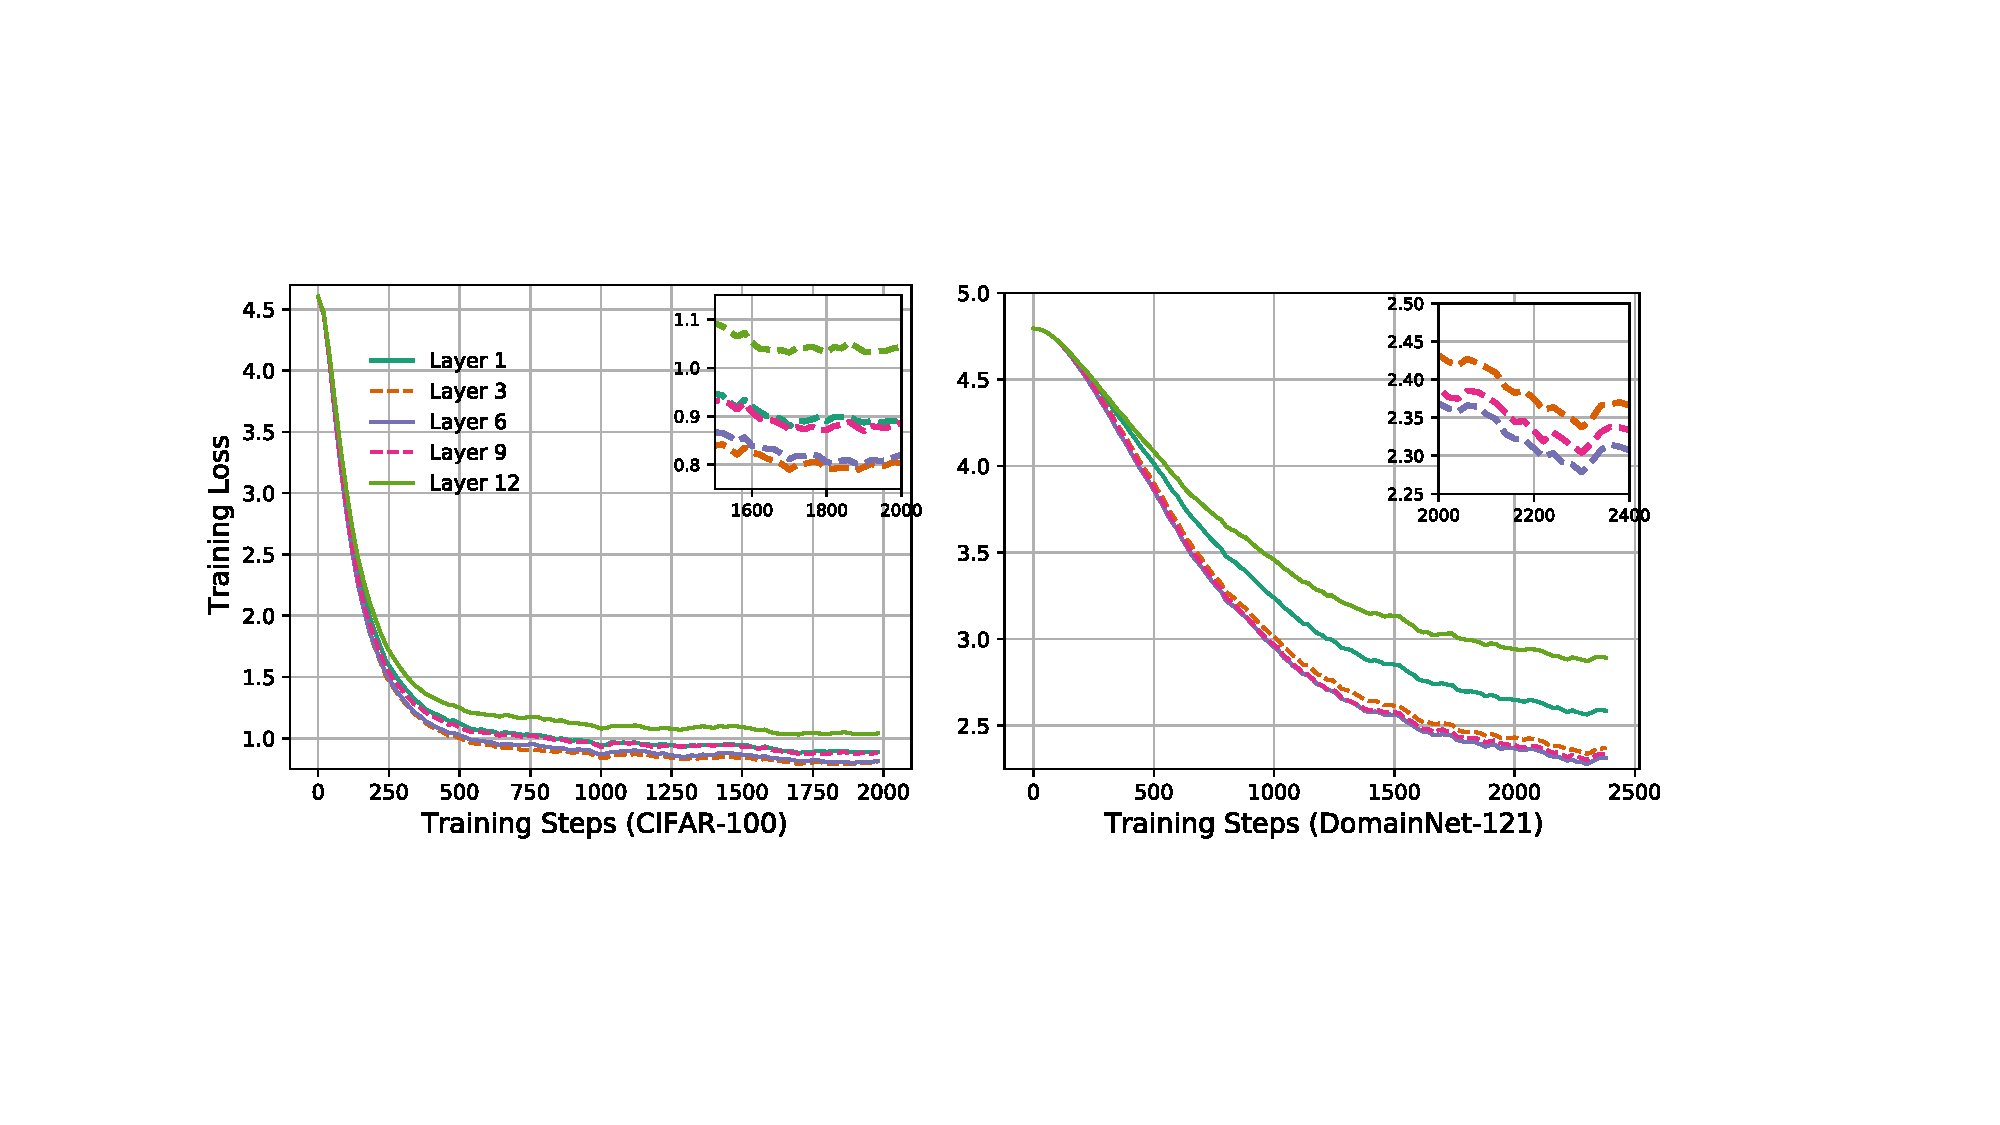
\includegraphics[width=0.49\textwidth]{figure/layerimportance-motivation.pdf}
% \vspace{-10pt}
\caption{{The convergence of fine-tuning different LoRA layers on ViT-base model in centralized settings across CIFAR100 and DomainNet-121 dataset.}}
\label{fig:layer_importance}
% \vspace{-100pt} 
\end{figure}



% We extend FIM-HLA to a dynamic version, in which the FIM scores $\Gamma^t$ are recalculated at each round. This approach improves fixed FIM scores by capturing the dynamic changes in layer importance throughout training.

\subsubsection{Randomized Geometrically-Defined Heterogeneous LoRA Allocation for the Intrinsic Layer Importance}\label{sec:GD-DPP-HLA}

{
In Fed-HeLLo, FIM-HLA is conducted every round to generate allocation maps for clients. However, during the early training rounds, FIM scores do not provide an accurate estimation about the training state of the global model.
% obtains layer importance by calculating the gradient norm of each LoRA layer. However, during the early training rounds, the gradient norm may not reliably reflect stable information about layer importance. 
To explore this, we conduct an experiment on LEDGAR dataset, comparing the convergence speed of our proposed FIM-HLA with a random allocation baseline, FedRA~\cite{su2023fedra}. As shown in Figure~\ref{fig:fim-drawback}, FIM-HLA achieves faster overall convergence compared to FedRA, but FedRA initially converges faster during the first 10 rounds. This discrepancy may result from FIM-HLA's difficulty in capturing meaningful layer importance information early in training. To address this issue, we introduce a HLA method that provides an effective initial LoRA allocation by considering intrinsic layer importance.}



{
The intrinsic layer importance represents the natural role of each layer in feature extraction~\cite{pan2024lisa,gao2024higher}. For example, different tasks and datasets often require models to focus on specific feature hierarchies, where shallow layers capture edges, textures, and spatial structures, deep layers extract semantic meaning, object relationships, and contextual understanding. Object-centric datasets such as CIFAR-100~\cite{krizhevsky2009learning} and ImageNet~\cite{deng2009imagenet} emphasize deep-layer semantic features, whereas datasets like the Describable Textures Dataset (DTD)~\cite{cimpoi2014describing} prioritize shallow-layer textural details.} 
% To address this aspect, we introduce a Randomized Geometrically-Defined HLA (RGD-HLA) strategy.}
%
Inspired by these, we propose a Geometrically-Defined HLA (GD-HLA) strategy. This strategy allocates trainable LoRA layers to clients according to specific {patterns} that are effective at the global level, where the patterns are designed to consider the intrinsic LoRA layers importance. Specifically, we define four GD-HLAs, each resulting in a distinct global allocation pattern: \textit{Triangle} ($\rhd$), \textit{Inverted Triangle} ($\lhd$), \textit{Bottleneck} ($\bowtie$), and \textit{Uniform} ($\approx$). In the \textit{Triangle} pattern ($\rhd$), clients prioritize training on shallower LoRA layers, allocating more resources to these layers due to their significant impact on coarse-grained feature modeling. In contrast, the \textit{Inverted Triangle} pattern ($\lhd$) focuses on deeper LoRA layers, emphasizing the development of the ability to handle more semantic features. The \textit{Bottleneck} pattern ($\bowtie$) represents a trade-off between these two allocations, acknowledging the significance of both shallow and deep LoRA layers in feature modeling~\cite{zeiler2014visualizing}. Finally, the \textit{Uniform} pattern ($\approx$) assigns uniform significance to features across all layers, resulting in a uniform allocation by randomly selecting $c_i$ layers. 

Each strategy corresponds to a specific allocation mask for clients $i$, formalized as follows:

\begin{align}\label{eq:gd-HLA-assign}
m_i^\rhd    & = \left\{\underbrace{1,\cdots,1}_{c_i},\underbrace{0,\cdots,0}_{l-c_i}\right\}, \nonumber\\
m_i^\lhd    & = \left\{\underbrace{0,\cdots,0}_{l-c_i},\underbrace{1,\cdots,1}_{c_i}\right\}, \\
m_i^{\bowtie} & = \left\{\underbrace{1,\cdots,1}_{\left \lceil {c_i}/{2}\right \rceil },\underbrace{0,\cdots,0}_{l-c_i},\underbrace{1,\cdots,1}_{\left \lfloor {c_i}/{2}\right \rfloor}\right\}, \nonumber\\
% m_i^{\approx} & = \left\{0,1\right\}^{l} \sim \text{Uniform}\left(\frac{c_i}{l}\right).
m_i^{\approx} & = \left\{0,1\right\}^{l} \sim \text{Uniform}\left(c_i/l\right).\nonumber
\end{align}

% \begin{figure}[t]
% \centering
% \includegraphics[width=0.45\textwidth]{figure/geo_HLA-631_10.pdf}
% % \vspace{-10pt}
% \caption{Example of the allocation of local trainable LoRA layers across 100 clients (with 60, 30, and 10 clients capable of training 6, 9, and 12 LoRA layers, respectively) under four different GD-HLA strategies.}
% \label{fig:geo_HLA}
% % \vspace{-100pt} 
% \end{figure}

% In Figure~\ref{fig:geo_HLA}, we illustrate the global geometrical pattern of GD-HLAs, represented by the number of clients allocated to train specific layers, for the ViT-base model~\cite{vaswani2017attention}, which consists of 12 transformer layers. We implement the GD-HLAs across 100 clients, categorized into three capability levels: 60 clients capable of fine-tuning 6 layers, 30 clients capable of fine-tuning 9 layers, and 10 clients capable of fine-tuning all 12 layers of LoRA. These patterns visually demonstrate the concept of GD-HLAs. For instance, in the \textit{Triangle} HLA strategy, all clients (100\%) fine-tune the $1$-st to $6$-th layers, 4 out of 10 clients (40\%) fine-tune the $7$-th to $9$-th layers, while only the most powerful clients, 1 out of 10 (10\%) fine-tune the $10$-th to $12$-th layers.

% being 33, 33, and 34, respectively. 
% We consider three computational capability levels of 100 clients, each capable of fine-tuning 6, 9, or 12 layers of LoRA layers, with the number of clients being 33, 33, and 34, respectively. 
% The GD-HLAs follow the approaches outlined previously, and once allocated, the trainable LoRA layers for each client remain fixed throughout the FL training process. During FL training, 10 out of 100 clients are randomly selected for each training round, and the total number of training rounds is set to 500. 
% To enhance visualization, we aggregate the number of \hu{appearances} for every 50 training rounds and represent the frequency of appearance for each layer during training with different colors in heatmaps (as shown in the upper part of Figure~\ref{fig:geo_HLA}). Additionally, 
% We display the frequency of appearances for each layer across the training rounds to illustrate the geometrical shapes for different strategies. 
% These patterns visually demonstrate the concept of GD-HLAs. For instance, in the \textit{Triangle} HLA strategy, all clients (100\%) fine-tune the $1$-st to $6$-th layers, 4 out of 10 clients (40\%) fine-tune the $7$-th to $9$-th layers, while only the most powerful clients, 1 out of 10 (10\%) fine-tune the $10$-th to $12$-th layers.

% \hu{overlapped with experiments.} Given the allocation masks generated using the GD-HLA before training, we conduct the federated FM fine-tuning, where 10 out of 100 clients are randomly selected for local training at each round. We report the accuracy of Fed-HeLLo using GD-HLAs on CIFAR-100 dataset~\cite{krizhevsky2009learning} after 500 rounds fine-tuning under various IID and Non-IID data settings in Figure~\ref{fig:geo_comparison} (refer to Table~\ref{tab:gd-HLA} for experimental setting details and more results).
% Based on the GD-HLAs discussed above, we evaluate all four methods on CIFAR-100~\cite{krizhevsky2009learning} with various IID and Non-IID scenarios, as shown in Figure~\ref{fig:geo_comparison} (for more results, refer to Section~\ref{exp:geoHLA}). 
% Zikai: 两个点：（1）和其他两个考虑但是不能充分利用computational resource or client information的方法相比，HLA对于non-iid data更加stable （2）不同的GD-HLA中间存在比较明显的performance gap 
% We compare GD-HLAs with two baseline methods: \textit{Straggler Learning} and \textit{Exclusive Learning}. Straggler Learning allocates $\min\{c_i\}_{i=1}^n$ trainable layer for all clients based on the straggler's resource capability. Exclusive Learning excludes clients that are unable to train all the LoRA layers. 
% In this scenario, only 34 clients are eligible to fine-tune all 12 layers, the rest of clients will be dropped during fine-tuning. 
% For GD-HLAs, we report their performance collectively as an interval, highlighting only the highest score among these four strategies at each data heterogeneity level using ``Upper''. We denote \textit{Triangle} HLA as Tri and \textit{Bottleneck} HLA as BoNe. The figure shows that although Exclusive Learning remains reasonable performance in IID and mild Non-IID data settings, its accuracy decreases significantly in extreme Non-IID settings. Straggler Learning is evidently sub-optimal and fails to provide favorable performance. Moreover, the performance gaps among GD-HLAs are non-trivial, emphasizing the importance of HLA design according to \hu{the significance of each layer}. 
% \hu{
% % \textit{Furthermore, Triangle HLA performs well on IID data, and Bottleneck HLA consistently achieves the best performance on Non-IID data}.
% \ul%{Based on these observations, we validate the first two guidelines we proposed, emphasizing the importance of considering heterogeneous clients and designing HLA strategies.} 
% \hl{I will leave a question here: SHOULD we put this discussion here? do you have to point out which GD-HLA is the best one for 4.3; DPP-HLA in 4.3 right now is generally modeled based on any prior GD-HLA; and in the experiments, you pick the best GD-HLA as the prior probability to conduct the experiments of DPP-HLA. }

% \subsection{Dynamic Prior-Probability-based and Fisher Information Matrix Score-based HLAs for Dynamic Layer Importance}\label{sec:dpp-HLA} 
% \textbf{Prior-Probability-based HLA - the Randomized Version of GD-HLAs.} 
% The GD-HLA strategy provides insights into designing HLA based on the significance of different LoRA layers to ensure the effectiveness of Fed-HeLLo framework. 
% In this section,
Here, we extend the fixed GD-HLA to a randomized version, named Randomized Geometrically-Defined HLA (RGD-HLA).
% By adopting a probabilistic approach, the system becomes more robust to fluctuations in input data or task demands, leading to smoother model training and potentially better learning outcomes. In RGD-HLA, the selected client $i$ receives a new allocation mask $m_i^t$ from the server in each round $t$ to determine which LoRA layers to train. 
% This allocation strategy is based on prior probabilities derived from GD-HLAs. 
Specifically, using the allocation maps $\{m_i^\star\}_{i=1}^n$ generated by a pre-defined GD-HLA strategy $\star$, a prior allocation probability for each layer $j$ is calculated as 
\begin{equation}\label{eqn:dpp-HLA1}
% $ 
g_{(j)}^{\star} = \frac{\sum_{i=1}^{n} m_{i,(j)}^{\star}}{\sum_{j=1}^l \sum_{i=1}^{n} {m_{i, (j)}^{\star}}},
% $
\end{equation}
where $\sum_{j=1}^l g_{(j)}^{\star} =1$. 
{
Based on the allocation probability distribution $\{g_1, g_2, \dots, g_l^{\star}\}$, the server conducts a random sampling by selecting $c_i$ LoRA layers without replacement to obtain the allocation map for each client $i$.} This approach introduces randomness into the allocation of trainable LoRA layers based on a geometrically-defined prior probability, allowing resource-constrained clients the chance to train different layers, which can potentially improve fine-tuning performance. Note that despite the randomness at the individual client level, the overall distribution of layer allocations across all clients adheres to a stable and predictable pattern predefined by $\star$.

% Despite the random local LoRA layers selection, the overall allocation across all clients results in the distribution defined by $\star$. 
% \ping{it would be better to emphasize that it performs in a stable manner although it uses random selection.} 

\begin{figure}[]
\centering
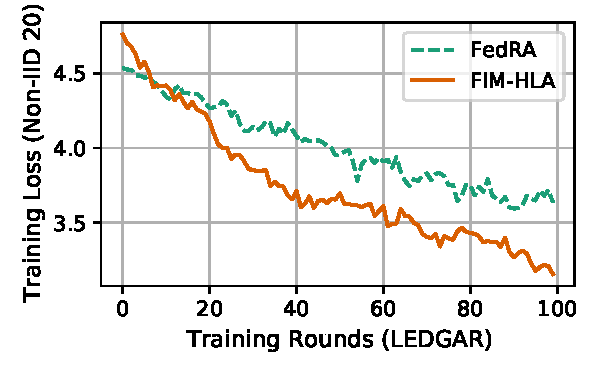
\includegraphics[width=0.38\textwidth]{figure/ledgar-losscurve-noniid-pat_20-locator-111.pdf}
% \vspace{-10pt}
\caption{{The convergence of FedRA and FIM-HLA on LEDGAR dataset.}}
\label{fig:fim-drawback}
% \vspace{-100pt} 
\end{figure}

% and a set of dummy clients $i^{-}\in[n^{-}], n^{-}=n$ that have same computational resources $c_{i^{-}}$ on each client. For each client $i^{-}$, the allocation mask will generated according to Equation~\eqref{eq:gd-HLA-assign} and computational capability level $c_{i^{-}}$, result in $m_{i^{-}}^{\star}:=\{m_{{i^{-}},(j)}^{\star}\}_{j\in\{1,\cdots,l\}}$. The proportion $g_{(j)}^{\star}$ for each layer $j$ is calculated as:
% \begin{equation}\label{eqn:dpp-HLA1}
% g_{(j)}^{\star} = \frac{\sum_{i^{-}=0}^{n^{-}-1} m_{i^{-},(j)}^{\star}}{\sum_{i^{-}=0}^{n^{-}-1} \sum{m_{i^{-}}^{\star}}}
% \end{equation}
% The term $\sum_{i^{-}=0}^{n^{-}-1} m_{i^{-},(j)}^{\star}$ denotes the total count of trainable LoRA layers across all dummy clients for layer $j$ in the context of the GD-HLA $\star$. Similarly, $\sum_{i^{-}=0}^{n^{-}-1} \sum{m_{i^{-}}^{\star}}$ represents the total count of trainable layers for all clients under the GD-HLA $\star$.


% enables us to \hu{adaptively adjust} the allocation of trainable LoRA layers based on prior-probability, thus enhancing the overall effectiveness of the FL learning process.

% \begin{figure}[t]
% \centering
% \includegraphics[width=0.95\linewidth]{figure/geo-fim-codesign.png}
% \caption{The scaled value of the minimum number of training samples for each layer with FIM-HLA from training rounds 100 to 500 on the LEDGAR dataset, along with their average. The distribution approximation curve illustrates the dynamic importance of layer training.}
% \label{fig:geo_fim_codesign}
% \end{figure}

% \end{algorithm}

% Table generated by Excel2LaTeX from sheet 'main-ClassSkew'
\begin{table*}[t]
% \color{NavyBlue}
% \arrayrulecolor{NavyBlue}
  \centering
  \caption{{Main results of Fed-HeLLo compared with baselines on CIFAR-100 dataset.}}
    \scalebox{1.1}{
    \begin{tabular}{c|c|cccc|cccc}
    \toprule[1pt]
    \multicolumn{2}{c|}{\multirow{2}[3]{*}{\textbf{Methods}}} & \multicolumn{4}{c|}{\textbf{Model Performance (Accuracy)}} & \multicolumn{1}{c}{\multirow{2}[0]{*}{\shortstack{\textbf{Avg Back. Comp.}\\\textbf{Cost (TFLOPs)}}}} & \multicolumn{1}{c}{\multirow{2}[0]{*}{\shortstack{\textbf{Avg Memory}\\\textbf{Cost (GB)}}}} & \multicolumn{1}{c}{\multirow{2}[0]{*}{\shortstack{\textbf{Avg Comm.}\\\textbf{Cost (MB/R)}}}} & \multicolumn{1}{c}{\multirow{2}[0]{*}{\shortstack{\textbf{Avg Training}\\\textbf{Time (Sec/R)}}}}  \\
\cmidrule{3-6}    \multicolumn{2}{c|}{} & \textbf{IID} & \textbf{20/1.0} & \textbf{10/1.0} & \textbf{Avg} &       &       &       &  \\
    \midrule
    Straggler & - & 68.15 & 60.48 & 55.88 & 61.50 &1.62       & 10.52 & 3.53      &6.38  \\ \midrule
    Exclusive & \multicolumn{1}{c|}{\multirow{6}[0]{*}{\shortstack{RoC\\6:3:1}}} & 78.33 & 4.49  & 7.13  & 29.98 &  3.25     & 12.29 & 4.71      &12.99\\
    HETLoRA &       & 80.10 & 64.36 & 53.20 & 65.88 & 3.22      & 12.25 & 2.85      &9.07  \\
    FlexLoRA &       & 44.77 & 44.36 & 38.40 & 42.51 & 3.22      & 12.25 & 57.12      &14.91  \\
    FLoRA &       & 3.56  & 2.39  & 2.88  & 2.94  & 3.22      & 12.25 & 5.47      &11.62  \\
    FedRA &       & 86.19 & 81.08 & 74.77 & 80.68 & 2.03      & 10.47 & 3.83      &10.17  \\
    \textbf{Fed-HeLLo} &       & \cellcolor[rgb]{ .749,  .749,  .749}86.50 & \cellcolor[rgb]{ .749,  .749,  .749}82.57 & \cellcolor[rgb]{ .749,  .749,  .749}78.49 & \cellcolor[rgb]{ .749,  .749,  .749}82.52 & 2.03      & 10.74 &3.83       &9.83  \\ \midrule
    Exclusive & \multicolumn{1}{c|}{\multirow{7}[0]{*}{\shortstack{RoC\\1:1:1}}}  & 85.20 & 81.14 & 70.26 & 78.86 & 3.25      & 12.19 & 4.71      & 11.87 \\
    HETLoRA &       & 85.56 & 81.06 & 69.69 & 78.77 & 3.23      & 12.26 & 3.41      &7.83  \\
    FlexLoRA &       & 42.35 & 40.47 & 36.32 & 39.71 & 3.23      & 12.26 & 57.67      &21.23  \\
    FLoRA &       & 4.04  & 3.58  & 2.29  & 3.30 & 3.23      & 12.26 & 11.53      & 12.92 \\
    FedRA &       & 87.06 & 84.05 & 78.51 & 83.20 & 2.45      & 11.08 &4.14       &9.52  \\
    \textbf{Fed-HeLLo} &       & \cellcolor[rgb]{ .749,  .749,  .749}87.11 & \cellcolor[rgb]{ .749,  .749,  .749}84.64 & \cellcolor[rgb]{ .749,  .749,  .749}79.76 & \cellcolor[rgb]{ .749,  .749,  .749}83.84 &2.45       & 11.19 &4.14       & 5.01 \\ \bottomrule[1pt]
    \end{tabular}%
    }
  \label{tab:main-cifar}%
  \arrayrulecolor{black}
\end{table*}%


% Table generated by Excel2LaTeX from sheet 'main-ClassSkew'
\begin{table*}[t]
% \color{NavyBlue}
% \arrayrulecolor{NavyBlue}
  \centering
  \caption{{Main results of Fed-HeLLo compared with baselines on LEDGAR dataset.}}
  \scalebox{1.1}{
    \begin{tabular}{c|c|cccc|cccc}
      \toprule[1pt]
    \multicolumn{2}{c|}{\multirow{2}[3]{*}{\textbf{Methods}}} & \multicolumn{4}{c|}{\textbf{Model Performance (Macro-F1)}} & \multicolumn{1}{c}{\multirow{2}[0]{*}{\shortstack{\textbf{Avg Back. Comp.}\\\textbf{Cost (TFLOPs)}}}} & \multicolumn{1}{c}{\multirow{2}[0]{*}{\shortstack{\textbf{Avg Memory}\\\textbf{Cost (GB)}}}} & \multicolumn{1}{c}{\multirow{2}[0]{*}{\shortstack{\textbf{Avg Comm.}\\\textbf{Cost (MB/R)}}}} & \multicolumn{1}{c}{\multirow{2}[0]{*}{\shortstack{\textbf{Avg Training}\\\textbf{Time (Sec/R)}}}}  \\
\cmidrule{3-6}    \multicolumn{2}{c|}{} & \textbf{IID} & \textbf{20/1.0} & \textbf{10/1.0} & \textbf{Avg} &       &       &       &  \\ \midrule
    Straggler & - & 56.82 & 51.05 & 44.05 & 50.64 & 1.62      &10.61       & 3.53      &6.58  \\ \midrule
    Exclusive & \multicolumn{1}{c|}{\multirow{6}[0]{*}{\shortstack{RoC\\6:3:1}}} & 61.25 & 44.72 & 28.48 & 44.81 & 3.25      & 12.38      & 4.71      &12.99  \\
    HETLoRA &       & 53.00 & 39.09 & 26.90 & 39.66 & 3.22      &12.35       & 2.87      &9.07  \\
    FlexLoRA &       & 29.08 & 4.08  & 5.01  & 12.72 &3.22       &12.35       & 57.13      &14.91  \\
    FLoRA &       & 0.06  & 0.04  & 0.08  & 0.06  & 3.22      &12.35       & 5.65      &11.62  \\
    FedRA &       & 66.74 & 61.73 & 55.71 & 61.39 & 2.04      &10.57       & 3.83      &10.17  \\
    \textbf{Fed-HeLLo} &       & \cellcolor[rgb]{ .749,  .749,  .749}67.00 & \cellcolor[rgb]{ .749,  .749,  .749}65.58 & \cellcolor[rgb]{ .749,  .749,  .749}61.04 & \cellcolor[rgb]{ .749,  .749,  .749}64.54 &  2.04     & 10.74      & 3.83      & 9.83 \\ \midrule
    Exclusive & \multicolumn{1}{c|}{\multirow{6}[0]{*}{\shortstack{RoC\\1:1:1}}} & 66.17 & 57.41 & 13.20 & 45.59 & 3.25      &12.38       & 4.71      & 8.45 \\
    HETLoRA &       & 62.88 & 54.50 & 45.78 & 54.38 &3.23       & 12.36      & 3.40      & 7.09 \\
    FlexLoRA &       & 30.95 & 1.19  & 1.83  & 11.32 &3.23       &12.36       & 57.66      & 13.33 \\
    FLoRA &       & 0.08  & 0.04  & 0.01  & 0.04  & 3.23      & 12.36      & 11.53      &12.18  \\
    FedRA &       & 66.63 & 62.61 & 56.39 & 61.87 & 2.45      & 11.16      & 4.13      & 6.54 \\
    \textbf{Fed-HeLLo} &       & \cellcolor[rgb]{ .749,  .749,  .749}66.75 & \cellcolor[rgb]{ .749,  .749,  .749}67.10 & \cellcolor[rgb]{ .749,  .749,  .749}64.27 & \cellcolor[rgb]{ .749,  .749,  .749}66.04 & 2.45      &11.28       & 4.13      & 5.75 \\
    \bottomrule[1pt]
  \end{tabular}%
    }
  \label{tab:main-ledgar}%
  \arrayrulecolor{black}
  
\end{table*}%

\subsubsection{Co-design of FIM-HLA and RGD-HLA}\label{sec:design-framework}

To consider both the dynamic and intrinsic importance of different LoRA layers, we co-design FIM-HLA and RGD-HLA to finalize our HLA strategy. 
% We need to address two key questions: (1) Determine the appropriate RGD-HLA strategy $\star$ for general use cases; and (2) Co-design the RGD-HLA and FIM-HLA strategies.
%
% To this end, we first study the relationship between the intrinsic and dynamic layer importance. 
% Specifically, we observe the minimum number of training samples allocated to each layer across clients using FIM-HLA, and report the results in Figure~\ref{fig:geo_fim_codesign}. 
% Note that the numbers are normalized with a min-max scaling. This value gives an insight of how important the layer that determined by FIM scores.
% Then, a second-degree quadratic fit is applied to approximate the shape of each line chart. 
% The results indicate that the \textit{Bottleneck}-shaped pattern becomes pronounced after 100 rounds, supporting the existence of the intrinsic layer importance and justifying the use of the \textit{Bottleneck} ($\bowtie$) pattern as a desirable prior allocation strategy\footnote{The ablation study on GD-HLA is detailed in Section~\ref{subsubsection:GD-HLA}}. Additionally, \textit{Bottleneck}-shaped patterns are observed to be adaptive and vary across different training rounds as shown in Figure~\ref{fig:geo_fim_codesign}, underscoring the need to consider the dynamic layer importance.
%
{
% Based on these findings, 
Specifically, our framework conducts RGD-HLA during the first $T_{\text{RGD}}$ rounds, which helps the model training to ``warm-start''.}
Then, at every $T_{\text{FIM}}$ rounds, FIM-HLA is used to update the allocation probability distribution for each LoRA layer. 
% This approach allows us to incorporate both the intrinsic and dynamic layer importance within the design of HLA.

\subsection{Computational Complexity and Communicational Cost}\label{sec:complexity}

{\textbf{Computational Complexity.}} 
% ?During the FL process, the computational complexity can be analyzed in terms of local training, model aggregation, and other operations. We compare our method with FedAvg~\cite{mcmahan2017communication}.
%
% For FedAvg, the computational cost is determined by standard forward and backward passes, which have a complexity of $O(\tau l d R N)$. In which $\tau$ represents the number of local epochs per round, $l$ represents the number of layers in the model, $d$ represents the number of parameters per layer, LoRA fine-tuning updates only $R$ low-rank parameters per selected layer, and $N$ represents the number of training samples per client.
% Thus, the computational cost scales linearly with the number of layers. Hence, the complexity for Fed-HeLLo is $O(\tau l/2 d R N)$ for clients with low-level resource.
%
% In addition, the server aggregates model updates from $s$ clients by computing a weighted average of the received parameters.
% For FedAvg, since each model update consists of $O(l d R)$ parameters, and the aggregation requires summing and averaging across $s$ clients, the aggregation complexity is $O(s l d R)$. However, for Fed-HeLLo, the aggregation complexity is $O(s l/2 d R)$.
%
% Additionally, there is a FIM score calculation cost for Fed-HeLLo, the complexity can be $dsa$, where $p$ is the total number of trainable parameters, $N_{\text{FIM}}$ be the number of samples for calculating FIM score, to compute the outer product of this gradient vector, which results in a $p\times p$ matrix, this part of complexity is represented as $O(l d R N_{\text{FIM}} +p^2N_{\text{FIM}})$.
%
% Overall, the computational complexity for Fed-HeLLo is $O(\tau l/2 d R N + s l/2 d R + l d R N_{\text{FIM}} +p^2N_{\text{FIM}})$, while FedAvg's computational complexity is represented as $O(\tau l d R N + l d R)$. As the $N_{\text{FIM}}$ is small, 
%
{During the FL process, the computational complexity can be analyzed in terms of local training, model aggregation, and other operations~\cite{wu2022node,zhou2022exact}. Here, we compare our method with FedAvg~\cite{mcmahan2017communication}.}

{During local training, the computational complexity is determined by forward and backward computations. For FedAvg, these operations have a computational complexity of $O(\tau l (d+R)^2 N s)$, where $\tau$ represents the number of local epochs per round, $l$ represents the number of layers, $d$ represents the number of parameters for pre-trained model in each layer, $R$ denotes the number of parameters for the LoRA layer, $N$ represents the number of training samples, and $s$ is the number of clients. The term $(d+R)^2$ represents the number of operations needed for matrix multiplications. 
For Fed-HeLLo, only $c$ LoRA layers are trainable, which results in a computational complexity of $O(\frac{\tau c (d+R)^2 N s}{l})$}.

{During model aggregation, the summing and averaging operations for Fed-HeLLo accounts for a computational complexity of $O(s l R)$, which is the same for FedAvg.}

{For Fed-HeLLo, there is an extra FIM score calculation cost every $T_{\text{FIM}}$ rounds on the server. The computational complexity is $O(\frac{l (d+R)^2 N_{\text{FIM}}T_{\text{FIM}}}{T} + \frac{R^2T_{\text{FIM}}}{T})$, where $N_{\text{FIM}}$ represents the number of samples used for calculating the FIM score, and $T$ represents the total training round. The first term is the computational complexity for obtaining the gradients. The second term represents the computational complexity of calculating the gradient norms.}

{Overall, the computational complexity of FedAvg is given by $O(\tau l (d+R)^2 N s + s l R)$. For Fed-HeLLo, it is $O(\frac{\tau c (d+R)^2 N s}{l} + s l R + \frac{l (d+R)^2 N_{\text{FIM}}T_{\text{FIM}}}{T} + \frac{R^2T_{\text{FIM}}}{T})$. Since $\frac{T_{\text{FIM}}}{T}$ is small, the last two terms can be neglected. Additionally, as aggregation operations are less computationally expensive than training, the second term is also omitted. As a result, Fed-HeLLo achieves reduced computational complexity by training fewer layers.}
% Then, we combine first term and thrid term of Fed-HeLLo's computational complexity. For example, if $c=\frac{l}{2}$, the computational complexity can be simplified as $\frac{\tau l (d+R)^2 (N+\frac{2N_{\text{FIM}}T_{\text{FIM}}}{\tau sT}) s}{lT}$, where $\frac{2N_{\text{FIM}}T_{\text{FIM}}}{\tau s T}$ is small and keeps a low overall computational complexity.}

{\textbf{Communication Cost}}
%
% {Since FedAvg transmits the full trainable model parameters from each client to the server and broadcasts back to all selected clients, the communication cost per round is $O(2s R)$. Our method involves transmitting the FIM scores, so the communication cost can be represented as $O(2 s R + s l)$.}
%
{In FedAvg, the full trainable LoRA layers are transmitted from clients to the server and then broadcast to all selected clients, resulting in a communication cost per round of $O(2 l R s)$. In Fed-HeLLo, allocation maps are transmitted every $T_{\text{FIM}}$ rounds, leading to a total communication cost of $O(2 c R s + \frac{l s T_{\text{FIM}}}{T})$. Since the communication cost for FIM scores is negligible, reducing the number of trainable LoRA layers decreases the communication cost, demonstrating the efficiency and practicality of our method in FL scenarios.}

\section{Experiments} 
In this section, we evaluate and compare the performance of our proposed method, Fed-HeLLo, with other baseline methods across various datasets and data distribution settings.

\subsection{Experimental Settings}\label{sec:exp}
We conduct experiments on both visual and language modalities. For visual tasks, we use CIFAR-100 dataset~\cite{krizhevsky2009learning} and a crafted version of DomainNet dataset~\cite{peng2019moment}, referred to as DomainNet-121. {For language tasks, we use LEDGAR dataset from LexGLUE~\cite{chalkidis-etal-2021-lexglue} for paragraph classification, as well as two instruction fine-tuning datasets: Natural Instruction~\cite{wang2022super} and Dolly-15K~\cite{ouyang2022training}.} We simulate three levels of data heterogeneity ranging from IID to extreme Non-IID by varying the data quantities, labels, or domains of clients. For example, a ``20/1.0'' Non-IID setting means that each client has samples from 20 categories, with quantities skewed by a Dirichlet distribution with $\alpha=1.0$; a ``25/D1'' Non-IID setting indicates that each client has 25 categories and one domain per category. 
% For FMs, we focus exclusively on models with a maximum of 1 million parameters~\cite{cho2023heterogeneous}. 

For visual tasks, we employ ViT-base~\cite{dosovitskiy2020image}, a 12-layer transformer encoder model designed for image processing. {For language tasks, we conduct experiments on three models. For LEDGAR dataset, we utilize BERT-base~\cite{devlin2019bert}, a 12-layer transformer model pre-trained on a comprehensive English corpus in a self-supervised manner. For the Natural Instruction and Dolly-15K dataset, we use the Llama-like model DataJuicer-1B~\cite{chen2024data} and OPT-1.3B~\cite{zhang2022opt} as the pre-trained models, respectively. For all these models, LoRA layers are applied to both the ``query'' and ``value'' modules in each transformer layer. The LoRA rank is set to 16 for ViT-base and BERT-base, and 8 for DataJuicer-1B and OPT-1.3B. The scaling parameter and dropout probability are set to 16 and 0.1, respectively.}

{For evaluation, we use top-1 accuracy for CIFAR-100 and DomainNet-121, Macro F1 score for LEDGAR~\cite{chalkidis-etal-2021-lexglue}, and Rouge-L score~\cite{lin2004rouge} for Natural Instruction and Dolly-15K. The batch sizes for local training on CIFAR100, LEDGAR, DomainNet-121, Natural Instruction, and Dolly-15K are 128, 128, 32, 1, and 1, respectively.}

% Table generated by Excel2LaTeX from sheet 'main-ClassSkew'
\begin{table*}[t]
% \color{NavyBlue}
% \arrayrulecolor{NavyBlue}
  \centering
  \caption{{Main results of Fed-HeLLo compared with baselines on Natural Instruction dataset.}}
  \scalebox{1.1}{
    \begin{tabular}{c|c|cccc|cccc}
      \toprule[1pt]
    \multicolumn{2}{c|}{\multirow{2}[3]{*}{\textbf{Methods}}} & \multicolumn{4}{c|}{\textbf{Model Performance (Rouge-L)}} & \multicolumn{1}{c}{\multirow{2}[0]{*}{\shortstack{\textbf{Avg Back. Comp.}\\\textbf{Cost (TFLOPs)}}}} & \multicolumn{1}{c}{\multirow{2}[0]{*}{\shortstack{\textbf{Avg Memory}\\\textbf{Cost (GB)}}}} & \multicolumn{1}{c}{\multirow{2}[0]{*}{\shortstack{\textbf{Avg Comm.}\\\textbf{Cost (MB/R)}}}} & \multicolumn{1}{c}{\multirow{2}[0]{*}{\shortstack{\textbf{Avg Training}\\\textbf{Time (Sec/R)}}}}  \\
\cmidrule{3-6}    \multicolumn{2}{c|}{} & \textbf{IID} & \textbf{20/1.0} & \textbf{15/1.0} & \textbf{Avg} &       &       &       &  \\ \midrule
    Straggler & - &59.71	&59.37	&59.11	&59.39  & 1.83      & 11.16      &  9.43     & 99.07 \\ \midrule
    Exclusive & \multicolumn{1}{c|}{\multirow{6}[0]{*}{\shortstack{RoC\\6:3:1}}} &59.58	&59.34	&59.42	&59.44 & 3.67      &12.40       & 12.58      &200.20  \\
    HETLoRA &       &60.65	&60.00	&60.21	&60.28 & 3.67      & 12.37      & 7.43      &153.40  \\
    FlexLoRA &      &61.93	&60.10	&\cellcolor[rgb]{ .749,  .749,  .749}60.86	&60.96  & 3.67      &12.37       & 806.44      &205.40  \\
    FLoRA &       &48.15	&48.69	&47.84	&48.22  & 3.67      & 12.37      & 7.36      &165.11  \\
    FedRA &      &60.91	&60.84	&60.50	&60.75  & 2.26      & 11.25      & 10.16      &101.46  \\
    \textbf{Fed-HeLLo} &       & \cellcolor[rgb]{ .749,  .749,  .749}66.18 & \cellcolor[rgb]{ .749,  .749,  .749}61.33 & 59.94 & \cellcolor[rgb]{ .749,  .749,  .749}62.48 & 2.26      & 11.28      & 10.16      &100.59  \\ \midrule
    Exclusive & \multicolumn{1}{c|}{\multirow{6}[0]{*}{\shortstack{RoC\\1:1:1}}} &63.03	&59.96	&59.58	&60.85 & 3.67      &12.40       & 12.58      &160.50  \\
    HETLoRA &       & 62.47	&60.39	&60.24	&61.03 &  3.67     & 12.38      & 8.92      &159.20  \\
    FlexLoRA &     & 61.63	&60.67	&60.49	&60.93  & 3.67      & 12.38      & 807.94      &191.79  \\
    FLoRA &       &48.05	&46.38	&48.88	&47.77 & 3.67      & 12.38      &  16.82     &143.36  \\
    FedRA &     & 61.84	  &61.41	&60.49	&61.24  & 2.76      &11.64       & 11.02      &98.55  \\
    \textbf{Fed-HeLLo} &       & \cellcolor[rgb]{ .749,  .749,  .749}68.22 & \cellcolor[rgb]{ .749,  .749,  .749}62.03 & \cellcolor[rgb]{ .749,  .749,  .749}60.89 & \cellcolor[rgb]{ .749,  .749,  .749}63.71 & 2.76      & 11.64      & 11.02      & 109.79 \\
    \bottomrule[1pt]
  \end{tabular}%
    }
  \label{tab:main-natural_instruction}%
  \arrayrulecolor{black}
  
\end{table*}%

% Table generated by Excel2LaTeX from sheet 'main-ClassSkew'
\begin{table*}[t]
% \color{NavyBlue}
% \arrayrulecolor{NavyBlue}

  \centering
  \caption{{Main results of Fed-HeLLo compared with baselines on Dolly-15K dataset.}}
  \scalebox{1.1}{
    \begin{tabular}{c|c|cccc|cccc}
      \toprule[1pt]
    \multicolumn{2}{c|}{\multirow{2}[3]{*}{\textbf{Methods}}} & \multicolumn{4}{c|}{\textbf{Model Performance (Rouge-L)}} & \multicolumn{1}{c}{\multirow{2}[0]{*}{\shortstack{\textbf{Avg Back. Comp.}\\\textbf{Cost (TFLOPs)}}}} & \multicolumn{1}{c}{\multirow{2}[0]{*}{\shortstack{\textbf{Avg Memory}\\\textbf{Cost (GB)}}}} & \multicolumn{1}{c}{\multirow{2}[0]{*}{\shortstack{\textbf{Avg Comm.}\\\textbf{Cost (MB/R)}}}} & \multicolumn{1}{c}{\multirow{2}[0]{*}{\shortstack{\textbf{Avg Training}\\\textbf{Time (Sec/R)}}}}  \\
\cmidrule{3-6}    \multicolumn{2}{c|}{} & \textbf{IID} & \textbf{3/1.0} & \textbf{1/1.0} & \textbf{Avg} &       &       &       &  \\ \midrule
    Straggler & - &57.89	&57.76	&57.83	&57.82   &  0.86     & 10.49      & 9.43      & 51.69 \\ \midrule
    Exclusive & \multicolumn{1}{c|}{\multirow{6}[0]{*}{\shortstack{RoC\\6:3:1}}} &57.98	&58.80	&57.92	&58.23  &  1.73     & 11.72      & 12.58      &108.41  \\
    HETLoRA &    &58.44	&58.92	&53.03	&56.79   & 1.73      & 11.70      &7.60       & 86.48 \\
    FlexLoRA &   &58.86	&58.84	&59.14	&58.94     & 1.73      & 11.70      & 806.62      &138.89  \\
    FLoRA &      &40.69	&41.47	&44.68	&42.28   & 1.73      & 11.70      & 7.58      & 114.42 \\
    FedRA &     &59.32	&59.28	&58.76	&59.12   & 1.06      & 10.57      & 10.14      &103.46  \\
    \textbf{Fed-HeLLo} &       & \cellcolor[rgb]{ .749,  .749,  .749}59.80 & \cellcolor[rgb]{ .749,  .749,  .749}59.90 & \cellcolor[rgb]{ .749,  .749,  .749}59.45 & \cellcolor[rgb]{ .749,  .749,  .749}59.71 &  1.06     & 10.61      & 10.14      &94.25  \\ \midrule
    Exclusive & \multicolumn{1}{c|}{\multirow{6}[0]{*}{\shortstack{RoC\\1:1:1}}} &59.38	&59.37	&58.58	&59.11  & 1.73      & 11.72      &  12.58     &131.39  \\
    HETLoRA &     & 59.36	&59.34	&59.08	&59.26  &  1.73     &11.71       & 9.45      &90.14  \\
    FlexLoRA &    &58.82	&58.98	&58.68	&58.82   & 1.73      & 11.71      & 808.47      &133.51  \\
    FLoRA &       &42.19	&44.72	&44.70	&43.87 &  1.73     &11.71       & 19.03      &112.37  \\
    FedRA &       &59.38	&59.38	&59.07	&59.27  &  1.39     &11.11       & 11.33      &104.44  \\
    \textbf{Fed-HeLLo} &       & \cellcolor[rgb]{ .749,  .749,  .749}59.41 & \cellcolor[rgb]{ .749,  .749,  .749}59.40 & \cellcolor[rgb]{ .749,  .749,  .749}59.20 & \cellcolor[rgb]{ .749,  .749,  .749}59.33 & 1.39      & 11.14      &11.33       & 104.48 \\
    \bottomrule[1pt]
  \end{tabular}%
    }
  \label{tab:main-dolly15k}%
  \arrayrulecolor{black}
\end{table*}%

{For the FL settings, we consider $n=100$ clients for classification tasks (CIFAR-100, LEDGAR, and DomainNet-121) and $n=50$ for instruction fine-tuning tasks (Natural Instruction and Dolly-15k) unless otherwise specified. The local epoch $\tau$ and the number of training rounds $T$ are set to 1 and 500 for classification tasks, and 1 and 25 for instruction fine-tuning tasks, respectively. At each round, the server randomly selects $s=10$ clients to perform local fine-tuning, using the AdamW optimizer as the local solver.}

{We consider two settings for the number of clients. In a practical scenario with more low-resource devices, the ratio of clients is set to 6:3:1, with each group capable of training $\frac{1}{2}$, $\frac{3}{4}$, or all LoRA layers, corresponding to three levels of resource capabilities. We also consider an evenly distributed case (1:1:1 ratio of clients), where clients are divided into three resource levels, each capable of training $\frac{1}{2}$, $\frac{3}{4}$, or all LoRA layers. 
For the proxy dataset used in FIM-HLA, we randomly sample 100, 50, 1000, 50, and 50 samples from the test dataset of CIFAR100, LEDGAR, DomainNet-121, Natural Instruction, and Dolly-15K datasets, respectively, and exclude these samples throughout the entire process to ensure fairness.
In classification experiments, we set both $T_{\text{RGD}}$ and $T_{\text{FIM}}$ to 50 for Fed-HeLLo, and $T_{\text{RGD}}$=0 and $T_{\text{FIM}}$=1 for FIM-HLA. In instruction fine-tuning experiments, we set  $T_{\text{RGD}}$=1 and $T_{\text{FIM}}$=2 for Fed-HeLLo, and same as before for FIM-HLA.}
% \footnote{We provide the detailed experimental settings in Appendix~\ref{sec:appendix-settings}.}.

\subsection{Baselines}
To demonstrate the effectiveness of Fed-HeLLo, we compare it with several baselines as follows:
% \textbf{Centralized Learning} is used to simulate the ideal scenario that fine-tuning full trainable layers on centralized datasets.
% \textbf{Inclusive Learning} simulates another ideal scenario where all clients are resource-sufficient and update the whole LoRA layers during local training, i.e., $c_i=12,\forall i\in[n]$.
% \textbf{Runner-up Learning} involves clients with middle-level computational capability, i.e., $c_i=9,\forall i\in[n]$. 
% Methods list above are not applicable to heterogeneous client scenarios with varying computational capabilities.
\textbf{Straggler Learning} allocates $\min\{c_i\}_{i=1}^n$ trainable layers for all clients based on the straggler's resource capability, i.e., in our case $c_i=\frac{l}{2}$, $\forall i\in[n]$.
\textbf{Exclusive Learning} excludes clients that are unable to train all LoRA layers.
\textbf{HETLoRA~\cite{cho2023heterogeneous}} is a federated LoRA-based fine-tuning framework that supports heterogeneous LoRA ranks across clients. 
{For HETLoRA, we align the number of clients across three levels of resource capabilities with our method's settings, with each group of clients capable of training LoRA layers at ranks 1, 4, or 16 for classification tasks and 1, 1, or 8 for instruction fine-tuning tasks.
{\textbf{FLoRA}}~\cite{wang2024flora} assigns lower ranks to resource-constrainted clients and shares stacked LoRA modules for updates.
{\textbf{FlexLoRA}}~\cite{bai2024flexlora} improves aggregation in rank-based methods using SVD.
}
\textbf{FedRA~\cite{su2023fedra}} is a federated LoRA-based fine-tuning framework that generates a random allocation map to allocate trainable LoRA layers to clients for each round. 

% Table generated by Excel2LaTeX from sheet 'furtherExp-NonIIDData'
\begin{table}[t]
% \arrayrulecolor{NavyBlue}
  \centering
  \caption{{Main results of Fed-HeLLo compared with baselines on DomainNet-121 dataset.}}
  \scalebox{1.1}{
    \begin{tabular}{c|c|cccc}
    \toprule[1pt]
    \multicolumn{2}{c|}{\multirow{2}[2]{*}{\textbf{Methods}}} & \multicolumn{4}{c}{\textbf{Model Performance (Accuracy)}} \\
    \cmidrule{3-6}    \multicolumn{2}{c|}{} & \textbf{IID} & \textbf{25/D1} & \textbf{15/D1} & \textbf{Avg} \\ \midrule
    % \multicolumn{3}{c|}{\textbf{Dataset/Model}} & \multicolumn{4}{c}{\textbf{DomainNet-121/ViT-base}}   \\
% \cmidrule{1-6}    \multicolumn{2}{c}{\textbf{Metric}} & \multicolumn{4}{c}{\textbf{Accuracy (\%)} $\uparrow$} &         \\
% \cmidrule{1-6}    \multicolumn{2}{c}{\textbf{(Methods/Client Settings)/DH}} & \textbf{IID} & \textbf{25/1} & \textbf{15/1} & \textbf{Avg}        &  \\
% \midrule
    Straggler & \multicolumn{1}{c|}{-} & 49.03 & 34.87 & 29.20 & 37.70     \\
    \midrule
    Exclusive & \multicolumn{1}{c|}{\multirow{6}[0]{*}{\shortstack{RoC\\6:3:1}}} & 54.04 & 29.69 & 21.43 & 35.05    \\
    HETLoRA &       & 54.43 & 27.98 & 13.52 & 31.97      \\
    {FlexLoRA} &      &{31.12}  &{3.41}  &{0.99}  &{11.84}     \\
    {FLoRA}    &      &{1.51}  &{1.15}  &{1.01}  &{1.22}   \\
    FedRA &       & 65.39 & 52.39 & 48.26 & 55.34  \\
    \textbf{Fed-HeLLo} &       & \cellcolor[rgb]{ .749,  .749,  .749}67.25 & \cellcolor[rgb]{ .749,  .749,  .749}54.44 & \cellcolor[rgb]{ .749,  .749,  .749}50.22 & \cellcolor[rgb]{ .749,  .749,  .749}57.30       \\
    \midrule
    Exclusive & \multicolumn{1}{c|}{\multirow{6}[0]{*}{\shortstack{RoC\\1:1:1}}} & 65.23 & 51.70 & 46.58 & 54.50       \\
    HETLoRA &       & 64.26 & 48.92 & 35.34 & 49.50      \\
    {FlexLoRA} &      &{23.05}  &{1.21}  &{1.21}  &{8.44}   \\
    {FLoRA} &         &{1.79}  &{1.01}  &{1.07}  &{1.29}   \\
    FedRA &       & 68.53 & 55.64 & 51.07 & 58.41  \\
    \textbf{Fed-HeLLo} &       & \cellcolor[rgb]{ .749,  .749,  .749}68.98 & \cellcolor[rgb]{ .749,  .749,  .749}58.01 & \cellcolor[rgb]{ .749,  .749,  .749}53.74 & \cellcolor[rgb]{ .749,  .749,  .749}60.24       \\
    \bottomrule[1pt]
    \end{tabular}%
    }
  \label{tab:main-domainnet121}%
  \arrayrulecolor{black}
  
\end{table}%

\subsection{Experimental Results}\label{exp:main-results}
We evaluate the effectiveness of our Fed-HeLLo framework on five datasets under three levels of data heterogeneity, comparing it with baseline methods. The main experimental results are summarized in Tables~\ref{tab:main-cifar}, \ref{tab:main-ledgar}, \ref{tab:main-natural_instruction}, \ref{tab:main-dolly15k} and \ref{tab:main-domainnet121}, where the best results among all methods are highlighted in \colorbox[rgb]{ .749,  .749,  .749}{grey}, and the average performance across all data settings is also reported. 
{Additionally, we provide a comparison of several resource indicators, including the average backward computational cost per step across all clients, average memory usage per step, average communication cost per round, and average wall-clock training time per round.
% DH represents the data heterogeneity level among all clients,
RoC represents the ratio of heterogeneous resource clients.}
% and ``10/100 Clients'' indicates that there are 100 clients, with the server randomly selecting 10 clients for each round of training. 

% We observe that as the degree of Non-IID increases, the performance of all methods drops significantly. 
% This highlights the sensitivity of federated FM fine-tuning to data heterogeneity and underscores the importance of considering practical data distribution when evaluating the performance of federated FM fine-tuning.

\textbf{Quantitative Results on CIFAR-100:} We compare our method Fed-HeLLo with two baseline methods (i.e., Straggler and Exclusive Learning) and four SOTA heterogeneous federated LoRA-based fine-tuning methods (i.e., HETLoRA, FlexLoRA, FLoRA, and FedRA). Table~\ref{tab:main-cifar} reports the comparison results. In CIFAR-100 experiments, Fed-HeLLo demonstrates substantial improvements across various settings. Under the 6:3:1 RoC distribution, Fed-HeLLo achieves an average accuracy of 82.52\%, surpassing Straggler Learning by +21.02\% and Exclusive Learning by +52.54\%. {Compared to the rank-based method HETLoRA, the performance gains are even more significant (+6.40\%, +18.21\%, +25.29\%) as the data heterogeneity becomes more extreme. FlexLoRA and FLoRA result in lower overall performance, indicating that their SVD and stacking techniques hinder the global model's convergence. This is likely due to their noise-alleviation aggregation being ineffective when not all LoRA layers are trainable.} Additionally, our method achieves substantial improvements over the SOTA method FedRA, demonstrating the effectiveness of leveraging both dynamic and intrinsic layer importance in our framework. Similarly, under the 1:1:1 RoC setting, our method continues to outperform other methods, achieving +1.25\% and +10.07\% improvements over FedRA and HETLoRA, respectively, in the ``10/1.0'' Non-IID setting. Notably, Exclusive Learning outperforms HETLoRA in this setting, indicating that rank-based method can be detrimental during training. These results underscore the robustness of Fed-HeLLo in effectively managing resource heterogeneity in CIFAR-100 dataset. {Regarding resource efficiency, under the 6:3:1 RoC distribution, rank-based methods such as HETLoRA, FlexLoRA, and FLoRA achieve minimal computational and memory savings compared to full LoRA layer fine-tuning. In contrast, our method reduces computational cost by 38.41\% and saves an average of 1.55 GB of memory. Additionally, our approach requires only 3.83 MB of communication per round, significantly lower than FlexLoRA, which needs to transmit full-rank matrices for each client.
}

\textbf{Quantitative Results on LEDGAR:} On LEDGAR dataset~\ref{tab:main-ledgar}, our method consistently demonstrates strong performance. Under the 6:3:1 RoC distribution, Fed-HeLLo improves the macro F1 score by +13.90\% compared to Straggler Learning and +19.73\% compared to Exclusive Learning. Notably, in the most extreme Non-IID scenario (10/1.0), Fed-HeLLo continues to outperform other methods, with a +5.33\% improvement over FedRA and a +34.14\% improvement over HETLoRA. {FlexLoRA and FLoRA also perform poorly in this scenario. It also indicates that these rank-based methods are not scalable to mid-sized FMs due to the limited prior information in the pre-trained weights.}
In the 1:1:1 RoC scenario, our method maintains all macro F1 scores above 60\%, and outperforms the SOTA methods HETLoRA and FedRA by +11.66\%, and +4.17\% on average, respectively.
These observations highlight Fed-HeLLo's ability to adapt to severe data distribution challenges. The results indicate that Fed-HeLLo excels in more balanced scenarios while remaining effective in environments with significant resource and data heterogeneity, making it a robust solution for complex datasets like LEDGAR. {Regarding resource efficiency, our method reduces the average backward computational cost by 1.18 TFLOPs compared to rank-based methods under the 6:3:1 RoC scenario and by 0.78 TFLOPs under the 1:1:1 RoC scenario. It increases average memory usage by only 0.13 GB compared to Straggler Learning under the 6:3:1 RoC distribution. However, as the number of low-resource devices increases, this gap becomes negligible. Additionally, our method decreases training time by 0.34 seconds and 0.79 seconds compared to the random allocation method FedRA under the 6:3:1 and 1:1:1 RoC distributions, respectively, benefiting from the designed HLA strategy.
}

{\textbf{Quantitative Results on Natural Instruction:} 
% We further discuss the performance on larger language models on instruction fine-tuning tasks. On Natural Instruction dataset with the 6:3:1 RoC distribution, our method obtain an extremely high performance on IID distribution with improvement of +18.03\%, +6.60\%, +6.47\%, +5.27\%, compared to FLoRA, Exclusive Learning, Straggler Learning, and HETLoRA, respectively. FedRA does not have a comparable performance in this case with a drop of -5.27\% compare to our method, due to the random allocated LoRA layers lead to an suboptimal convergence speed. FlexLoRA obtain a much higher performance compared to the scenario under mid-size FMs, while our method still outperform it by a large margin of +4.25\%. In the Non-IID scenario (15/1.0), our method shows a slight drop compared to FlexLoRA, it is because our method requires more rounds of training to learn an optimal LoRA layer allocation specially under Non-IID data distribution (refer to our discussion on Section~\ref{sec:visualization_of_training}). 
We further evaluate performance on larger language models for instruction fine-tuning tasks, as presented in Table~\ref{tab:main-natural_instruction}. On Natural Instruction dataset with the 6:3:1 RoC distribution, our method achieves exceptionally high performance on IID scenario, outperforming FLoRA, Exclusive Learning, Straggler Learning, and HETLoRA by +18.03\%, +6.60\%, +6.47\%, and +5.27\%, respectively. However, our method outperforms FedRA by +5.27\% with our HLA design. While FlexLoRA performs reasonably well, our method still surpasses it by a considerable margin of +4.25\%. In the Non-IID scenario (15/1.0), our method shows a slight performance drop compared to FlexLoRA, as it may requires more training rounds to optimize LoRA layer allocation under Non-IID data distributions (see Section~\ref{sec:visualization_of_training} for further discussion).
% Considering the average backward computational cost, our method decrease by 1.41 TFLOPs compared to rank-based methods, decreasing enlarge linearly as the batch size increases (it is 1 in our case). Our method decrease by 1.09 GB of average memory cost compared to rank-based methods, and increase by 0.12 GB when it compares to Straggler Learning. As for the average communication cost, our method keeps it low as we only required to uplink the allocated LoRA layer's parameters. While FlexLoRA requires to downlink the full rank matrix of LoRA layers, it requires much more communication costs. Our method has a good balance between training time and model performance, and it only increases by 1.52 seconds and 10.72 seconds compared to Straggler Learning under the 6:3:1 and 1:1:1 RoC distributions, respectively.
Regarding computational efficiency, our method reduces the average backward computational cost by 1.41 TFLOPs compared to rank-based methods, with the reduction scaling linearly as batch size increases (set to 1 in our case). It also lowers average memory usage by 1.09 GB compared to rank-based methods and only increases it by 0.12 GB relative to Straggler Learning. In terms of communication cost, our method remains efficient since only the trainable LoRA layer’s parameters need to be uploaded, whereas FlexLoRA requires downloading the full-rank matrix of LoRA layers, resulting in significantly higher communication overhead. Additionally, our method strikes a balance between training time and model performance, increasing training time by only 1.52 seconds compared to Straggler Learning under the 6:3:1 distribution.
}

{\textbf{Quantitative Results on Dolly-15K:} 
% Dolly-15K provides a real-world scenario of human generated prompt-response pairs. According to Table~\ref{tab:main-dolly15k}, our method achieves the best model performances among all compared methods and all RoC distributions. Notably, our method maintain a stable performance on both IID and Non-IID settings. Specifically, under the 6:3:1 RoC distribution, our method increase the average Rouge-L score by +1.89\%, +2.92\%, +17.43\% compared to Straggler Learning, HETLoRA, and FLoRA. FlexLoRA decreases the performance of -0.77\% compared to our method even uses SVD to obtain the LoRA layer parameters. Compared to random allocation method FedRA, our method increase by +0.59\% even under the competitive baseline performance. 
Dolly-15K presents a real-world scenario with human-generated prompt-response pairs. As shown in Table~\ref{tab:main-dolly15k}, our method outperforms all compared approaches across all RoC distributions, consistently maintaining stable performance in both IID and Non-IID settings. Under the 6:3:1 RoC distribution, our method improves the average Rouge-L score by +1.89\%, +2.92\%, and +17.43\% compared to Straggler Learning, HETLoRA, and FLoRA, respectively. Despite using SVD to obtain LoRA layer parameters, FlexLoRA still falls behind, our method surpasses it by +0.77\% in performance. Our method achieves a +0.59\% improvement compared to FedRA.
The resource efficiency trends remain consistent under Dolly-15K dataset. Our method reduces the average backward computational cost by 0.67 TFLOPs and 0.34 TFLOPs compared to rank-based methods under the 6:3:1 RoC and 1:1:1 RoC distributions, respectively. It also lowers average memory usage by 1.09 GB and 0.57 GB for the two distributions. Additionally, our method maintains a low average communication cost compared to Exclusive Learning and FlexLoRA, while achieving a balanced trade-off in training time, requiring only 94.25 and 104.48 seconds per training round.
}

\textbf{Quantitative Results on DomainNet-121:} In DomainNet-121 experiments, as shown in Table~\ref{tab:main-domainnet121}, Fed-HeLLo further demonstrates its effectiveness, particularly in handling Non-IID data. Under the 6:3:1 RoC distribution, Fed-HeLLo achieves an average accuracy of 57.30\%, outperforming Straggler Learning by +19.60\% and Exclusive Learning by +22.25\%. In the 1:1:1 RoC setting, Fed-HeLLo continures to outperform baseline methods, with a +9.09\% improvement over HETLoRA in the ``25/1'' Non-IID scenario and a +6.31\% increase over Exclusive Learning. Even in the most challenging ``15/1'' Non-IID setting, Fed-HeLLo maintains its advantage, outperforming HETLoRA by +18.40\%. 
On average, Fed-HeLLo outperforms FedRA by +1.96\% and +1.83\% in the 6:3:1 and 1:1:1 RoC settings, respectively.
{FlexLoRA and FLoRA perform poorly on mid-sized model, showing significant performance drops across both RoC distributions.}
These results on the DomainNet-121 dataset reinforce Fed-HeLLo's capability to handle diverse and challenging FL environments, ensuring high performance even under extreme conditions.

\subsection{Visualization of the Training Process}\label{sec:visualization_of_training}
\begin{figure*}[t]
% \vspace*{-10pt}
\centering
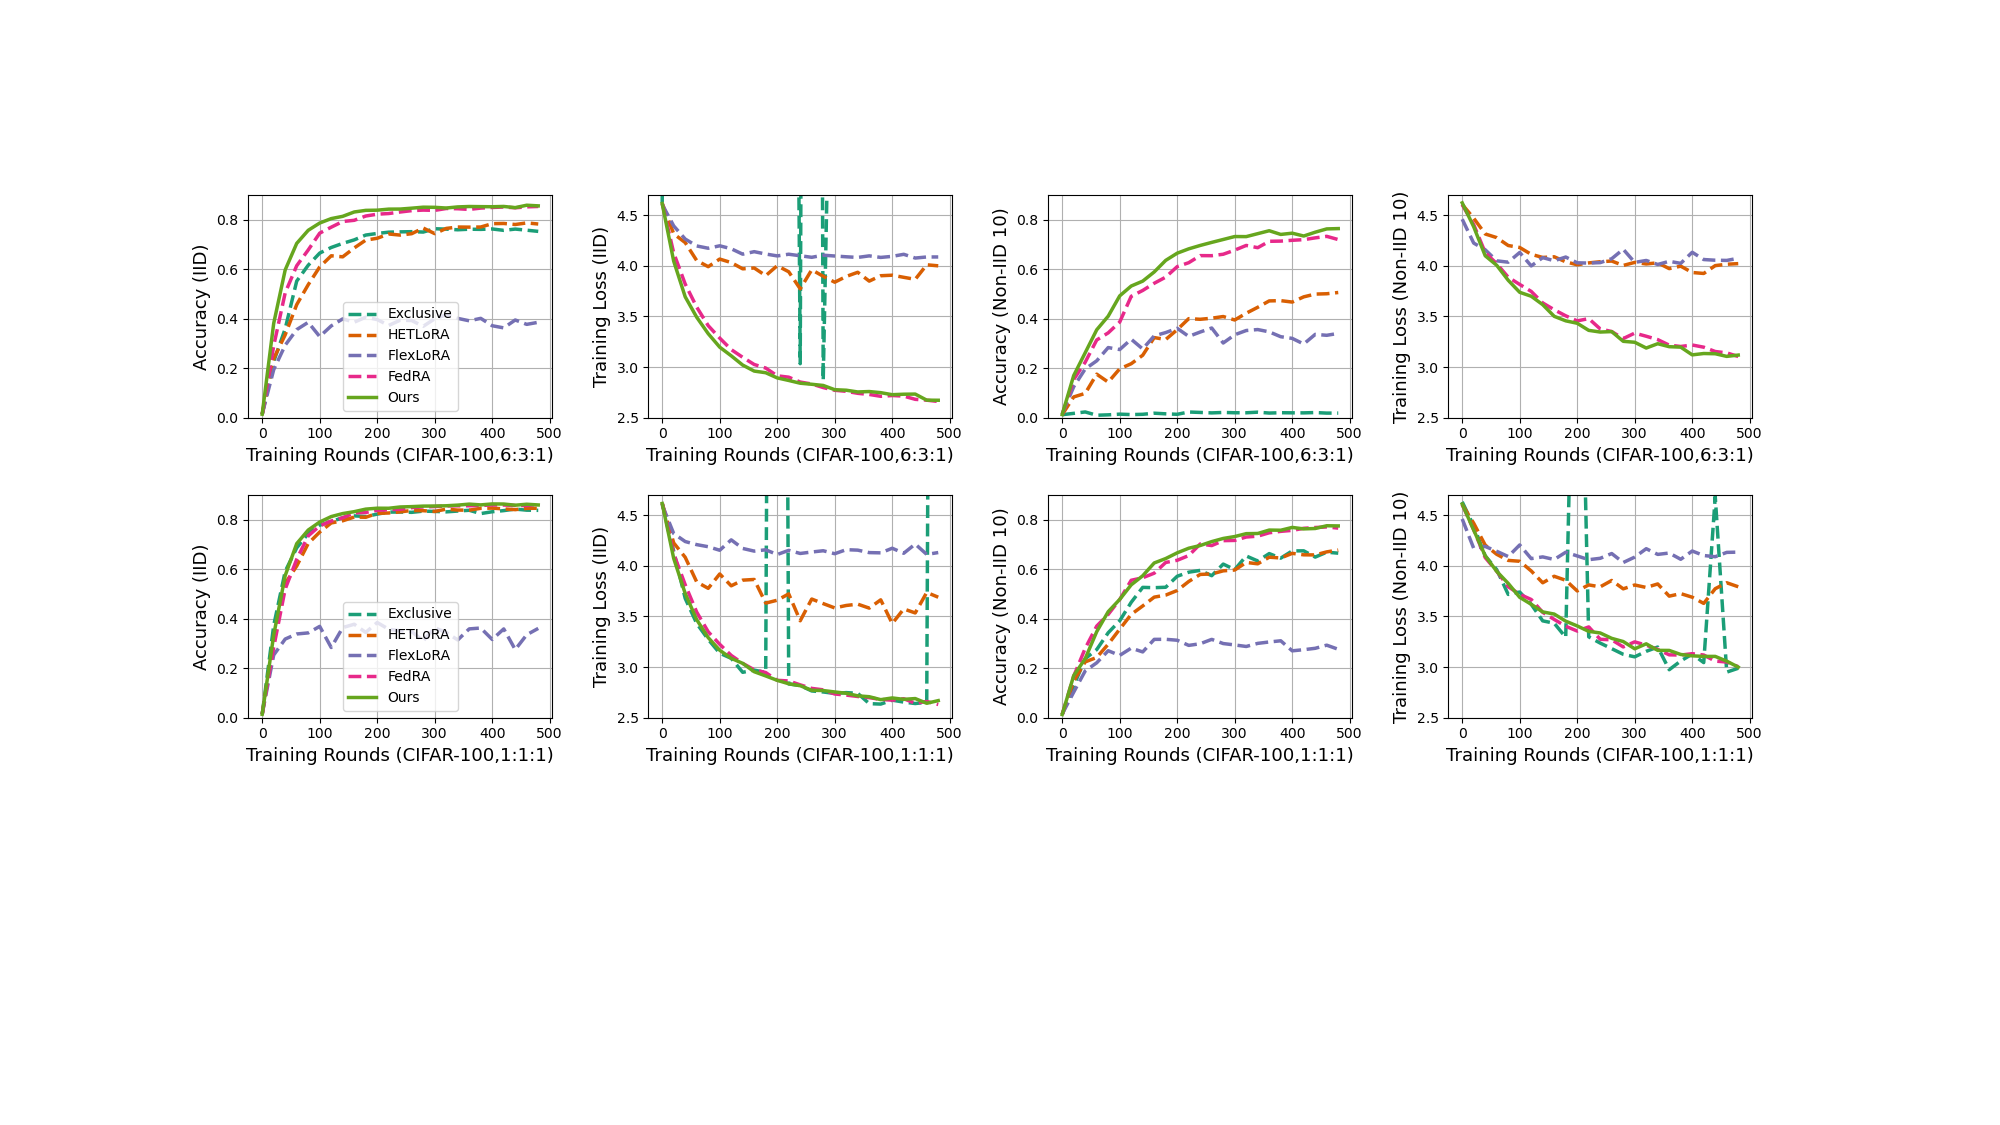
\includegraphics[width=0.9\linewidth]{figure/accuracy-loss-cifar100.pdf}
% \vspace*{-15pt}
\caption{{The accuracy and training loss with respect to training rounds on CIFAR-100 dataset, across different data and device settings.}}
\label{fig:acc-loss-cifar100}
% \vspace*{-10pt}
\end{figure*}

{
% We visualize the accuracy and loss curve during training for several baseline and our methods on CIFAR-100 datasets. As shown in Figure~\ref{fig:acc-loss-cifar100}, the first row we show the RoC of 6:3:1 and the second row is the RoC of 1:1:1. The first two plots for each row are the accuracy and training loss on IID data distribution, while the later two plots are on Non-IID data distribution settings. 
% We compare our method with Exclusive Learning, HETLoRA, FlexLoRA, and FedRA, other baseline methods we discuss above show a poor convergence pattern, so we omit from this evaluations. 
We visualize the accuracy and loss curves during training with four methods (i.e., Exclusive Learning, HETLoRA, FlexLoRA, and FedRA) and our approach on CIFAR-100 dataset. As shown in Figure~\ref{fig:acc-loss-cifar100}, the first row presents results under the 6:3:1 RoC distribution, while the second row corresponds to the 1:1:1 RoC distribution. For each row, the first two plots illustrate accuracy and training loss under an IID data distribution, whereas the latter two depict results under a Non-IID setting.
% We omit other baselines due to their poor convergence behavior.
% Taking the accuracy and training loss curves under the 6:3:1 RoC distribution in an IID setting as the example, The plots show that our method (green solid line) achieves the highest accuracy and converges faster compared to other approaches. Notably, FlexLoRA (blue dashed line) exhibits significantly lower accuracy, indicating poor performance in this setting. FedRA (pink dashed line) and HETLoRA (orange dashed line) converge more slowly than our method, with HETLoRA stabilizing at a lower accuracy. The right plot illustrates training loss, where our method consistently reduces loss faster and reaches a lower final value, demonstrating better convergence. Exclusive learning (deep green dashed line) shows instability with sudden fluctuations at the beginning of the training rounds, suggesting training instability under this distribution. These results highlight the effectiveness of our approach in achieving both superior accuracy and stable training dynamics compared to existing methods.
Taking the accuracy and training loss curves under the 6:3:1 RoC distribution in an IID setting as an example, the plots show that our method (green solid line) achieves the highest accuracy and converges faster than other approaches. Notably, FlexLoRA (blue dashed line) exhibits significantly lower accuracy, indicating poor performance in this setting. FedRA (pink dashed line) and HETLoRA (orange dashed line) converge more slowly than our method, with HETLoRA stabilizing at a lower accuracy. The right plot illustrates training loss, where our method consistently reduces loss faster and reaches a lower loss, demonstrating better convergence. Exclusive Learning (deep green dashed line) shows instability with sudden fluctuations at the beginning of the training rounds, suggesting instability under this distribution. These results highlight the effectiveness of our approach in achieving both superior accuracy and stable training convergence compared to existing methods.
% However, when it comes to the Non-IID setting of 6:3:1 RoC distrubiton, the convergence of our method is slightly slower than other methods at the beginning, which lead to the issue we demostrate in the main results on Natural Instruction dataset.
% For the RoC distribution of 1:1:1, the performance gaps shrink slightly, however our methods are still outperform other baseline methods.
In the Non-IID setting of the 6:3:1 RoC distribution, our method converges slightly slower than FlexLoRA at the beginning, which aligns with the issue observed in the main results on the Natural Instruction dataset. Under the 1:1:1 RoC distribution, the performance gaps narrow slightly, but our method still outperforms other approaches, maintaining higher accuracy and better convergence stability.
} 

\subsection{Ablation Study}\label{exp:ablation-results}
\subsubsection{Cross-silo Setting Evaluation}
% \textbf{Impact of different client settings.} 

% Table generated by Excel2LaTeX from sheet 'furtherExp-cross-silo'
\begin{table}[t]
% \arrayrulecolor{NavyBlue}
  \centering
  \caption{{Cross-silo evaluation on CIFAR-100 with 20 clients and two RoC settings.}}
  \scalebox{0.95}{
    \begin{tabular}{c|c|cccc}
    \toprule[1pt]
    \multicolumn{2}{c|}{\textbf{Dataset/Model}} & \multicolumn{4}{c}{\textbf{CIFAR-100/ViT-base}} \\
    \midrule    \multicolumn{2}{c|}{\textbf{Metric}} & \multicolumn{4}{c}{\textbf{Accuracy (\%)} $\uparrow$} \\
    \midrule
    \multicolumn{2}{c|}{\textbf{(Methods/Client Settings)/DH}} & \textbf{IID} & \textbf{20/1.0} & \textbf{10/1.0} & \textbf{Avg} \\
    \midrule
    Straggler & \multicolumn{1}{c|}{-} & 72.73 & 56.92 & \cellcolor[rgb]{ .749,  .749,  .749}46.01 & 58.55 \\
    \midrule
    Exclusive & \multicolumn{1}{c|}{\multirow{6}[0]{*}{\shortstack{RoC\\6:3:1}}} & 79.26 & 31.70 & 14.31 & 41.75 \\
    HETLoRA &       & 81.92 & 32.63 & 17.50 & 44.01 \\
    {FlexLoRA} & &{38.57}       &{15.06}  &{10.22}  &{21.27}   \\
    {FLoRA} &    &{2.12}  &{1.28}  &{1.62}  &{1.67}  \\
    FedRA &       & 86.19 & 68.03 & 3.00 & 52.40 \\
    \textbf{Fed-HeLLo} &       & \cellcolor[rgb]{ .749,  .749,  .749}86.63 & \cellcolor[rgb]{ .749,  .749,  .749}69.29 & 6.49  & \cellcolor[rgb]{ .749,  .749,  .749}54.14 \\
    \midrule
    Exclusive & \multicolumn{1}{c|}{\multirow{6}[0]{*}{\shortstack{RoC\\1:1:1}}} & 84.98 & 54.70 & 4.98  & 48.22 \\
    HETLoRA &       & 86.60 & 60.89 & 41.92 & 63.13 \\
    {FlexLoRA} &       &{45.51}  &{16.69}  &{2.44}  &{21.54}  \\
    {FLoRA} &       &{2.99}  &{1.68}  &{1.86}  &{2.17}  \\
    FedRA &       & 87.64 & 74.68 & 53.28 & 71.86 \\
    \textbf{Fed-HeLLo} &       & \cellcolor[rgb]{ .749,  .749,  .749}88.22 & \cellcolor[rgb]{ .749,  .749,  .749}75.09 & \cellcolor[rgb]{ .749,  .749,  .749}56.27 & \cellcolor[rgb]{ .749,  .749,  .749}73.19 \\
    \bottomrule[1pt]
    \end{tabular}%
    }
  \label{tab:abl-num-client}%
  \arrayrulecolor{black}
  
\end{table}%

Here, we conduct an ablation study to evaluate the stability of our proposed method under cross-silo client settings. 
% In Table~\ref{tab:abl-num-client}, we evaluate Fed-HeLLo with only 20 clients, sampling 4 clients per round, to model the cross-silo settings. From the experiment on fewer clients, we observe that a smaller number of clients leads to deteriorated overall performance compared to the 100 client one. 
% For baseline methods, Exclusive Learning experiences a significant performance drop of 47.56\% from IID to Non-IID settings (i.e., 20/1.0), indicating more sensitivity with fewer clients.
Table~\ref{tab:abl-num-client} presents the cross-silo evaluation results on CIFAR-100 dataset using the ViT-base model, with 20 clients under two different RoC settings: 6:3:1 and 1:1:1. The table compares the performance of different methods across IID and two Non-IID scenarios (20/1.0 and 10/1.0). Under the 6:3:1 RoC setting, Fed-HeLLo significantly outperforms the other methods, achieving the highest average accuracy of 54.14\%. Specifically, Fed-HeLLo reaches 86.63\% accuracy in the IID case, outperform FedRA by +0.44\% and HETLoRA by +4.71\%. In the 20/1.0 Non-IID scenario, Fed-HeLLo achieves an accuracy of 69.29\%, which is +37.59\% higher than Exclusive Learning. However, all fix methods diverge in the ``10/1.0'' Non-IID case, showing low accuracies under 20\%, which may be a result from the imbalance of data among clients and heterogeneous client's model updates in this extreme Non-IID scenario. Under the 1:1:1 RoC setting, Fed-HeLLo continues to lead, achieving the highest average accuracy of 73.19\%. In the IID scenario, Fed-HeLLo reaches 88.22\% accuracy, which is +0.58\% better than FedRA and +3.24\% better than Exclusive Learning. In the 20/1.0 Non-IID case, Fed-HeLLo achieves an accuracy of 75.09\%, which is +0.41\% higher than FedRA and +14.20\% higher than HETLoRA. For the 10/1.0 Non-IID case, Fed-HeLLo's accuracy drops to 56.27\%, yet it outperforms FedRA by +2.99\% and HETLoRA by +14.35\%. {FlexLoRA and FLoRA perform even worse in cross-silo settings, demonstrating poor generalization to both the number of clients and mid-size FMs.}

\subsubsection{GD-HLA Evaluation}\label{subsubsection:GD-HLA}

% Table generated by Excel2LaTeX from sheet 'geo-ablation'
\begin{table}[t]
  \centering
  \caption{GD-HLA evaluation on CIFAR-100 dataset with two client settings: 100 clients with a RoC of 6:3:1, and 20 clients with a RoC of 1:1:1.}
  \scalebox{0.9}{
    \begin{tabular}{c|c|c|cccc}
    \toprule[1pt]
    \multicolumn{3}{c|}{\textbf{Dataset/Model}} & \multicolumn{4}{c}{\textbf{CiFAR-100/ViT-base}} \\
    \midrule
    \multicolumn{3}{c|}{\textbf{Metric}} & \multicolumn{4}{c}{\textbf{Accuracy (\%)} $\uparrow$} \\
    \midrule
    \multicolumn{3}{c|}{\textbf{(Methods/Client Settings)/DH}} & \textbf{IID} & \textbf{20/1.0} & \textbf{10/1.0} & \textbf{Avg} \\
    \midrule
    Triangle ($\rhd$) & \multicolumn{1}{c|}{\multirow{4}[2]{*}{\shortstack{10/100\\Clients}}} & \multicolumn{1}{c|}{\multirow{4}[1]{*}{\shortstack{RoC\\6:3:1}}} & 84.02 & 53.51 & 54.18 & 63.90 \\
    In-Triangle ($\lhd$) &       &       & 78.50 & 69.03 & 58.47 & 68.66 \\
    Uniform ($\approx$) &       &       & 84.12 & 70.85 & 55.83 & 70.26 \\
    \textbf{Bottleneck ($\bowtie$)} &       &       & \cellcolor[rgb]{ .749,  .749,  .749}84.16 & \cellcolor[rgb]{ .749,  .749,  .749}78.19 & \cellcolor[rgb]{ .749,  .749,  .749}71.02 & \cellcolor[rgb]{ .749,  .749,  .749}77.79 \\
    \midrule
    Triangle ($\rhd$) & \multicolumn{1}{c|}{\multirow{4}[0]{*}{\shortstack{4/20\\Clients}}} & \multicolumn{1}{c|}{\multirow{4}[0]{*}{\shortstack{RoC\\1:1:1}}} & 87.29 & 64.75 & 6.30 & 52.78 \\
    In-Triangle ($\lhd$) &       &       & 85.76 & 66.64 & 2.34  & 51.58 \\
    Uniform ($\approx$) &       &       & 87.15 & 62.18 & 2.00 & 50.44 \\
    \textbf{Bottleneck ($\bowtie$)} &       &       & \cellcolor[rgb]{ .749,  .749,  .749}87.50 & \cellcolor[rgb]{ .749,  .749,  .749}70.54 & \cellcolor[rgb]{ .749,  .749,  .749}38.18 & \cellcolor[rgb]{ .749,  .749,  .749}65.41 \\
    \bottomrule[1pt]
    \end{tabular}%
    }
  \label{tab:abl-geo}%
\end{table}%

Table~\ref{tab:abl-geo} illustrates the performance evaluation of GD-HLA on CIFAR-100 dataset, comparing four HLA patterns: \textit{Triangle}, \textit{Inverted-Triangle}, \textit{Uniform}, and \textit{Bottleneck}, under two client settings: 100 clients with a 6:3:1 RoC and 20 clients with a 1:1:1 RoC. In the 100 client, 6:3:1 RoC scenario, the \textit{Bottleneck} HLA pattern consistently outperforms the others, achieving the highest average accuracy of 77.79\%. Specifically, \textit{Bottleneck} records an accuracy of 84.16\% in the IID setting, slightly surpassing \textit{Triangle} and \textit{Uniform}, which achieve 84.02\% and 84.12\% accuracy, respectively. In the Non-IID case (20/1.0), \textit{Bottleneck} again leads with 78.19\% accuracy, outperforming \textit{Uniform} by +7.34\%, \textit{In-Triangle} by +9.16\%, and \textit{Triangle} by +24.68\%. This trend continues in the 10/1.0 Non-IID case, where \textit{Bottleneck} achieves 71.02\% accuracy, outperforming \textit{Uniform} by +15.19\%, \textit{In-Triangle} by +12.55\%, and \textit{Triangle} by +16.84\%.
% We observe that, although the second-degree quadratic fit in Figure~\ref{fig:geo_fim_codesign} is slightly higher in the deep layers compared to shallow layers, the \textit{In-Triangle} pattern does not perform as well. This further demonstrating that both shallow and deep layers are crucial for feature modeling.
In the 20 client, 1:1:1 RoC scenario, \textit{Bottleneck} HLA continues to outperforms other GD-HLA strategies, achieving an average accuracy of 65.41\%. Specifically, \textit{Bottleneck} achieves an accuracy of 87.50\% in the IID scenario, slightly higher than \textit{Triangle} and \textit{Uniform}, which recorded 87.29\% and 87.15\%, respectively. However, in the Non-IID (20/1.0) scenario, \textit{Bottleneck's} accuracy drops to 70.54\%, yet it remains higher than \textit{Uniform} by +8.36\%, \textit{In-Triangle} by +3.90\%, and \textit{Triangle} by +5.79\%. For the extreme Non-IID (10/1.0) case, \textit{Bottleneck} records an accuracy of 38.18\%, outperforming the other patterns by a significant margin, indicating its effectiveness in handling high degrees of Non-IID data.


\subsubsection{The Dynamic and Intrinsic Layer Importance Evaluation}\label{subsubsec:intrinsic-dynamic-layer-importance}

\begin{figure}[t]
% \vspace*{-10pt}
\centering
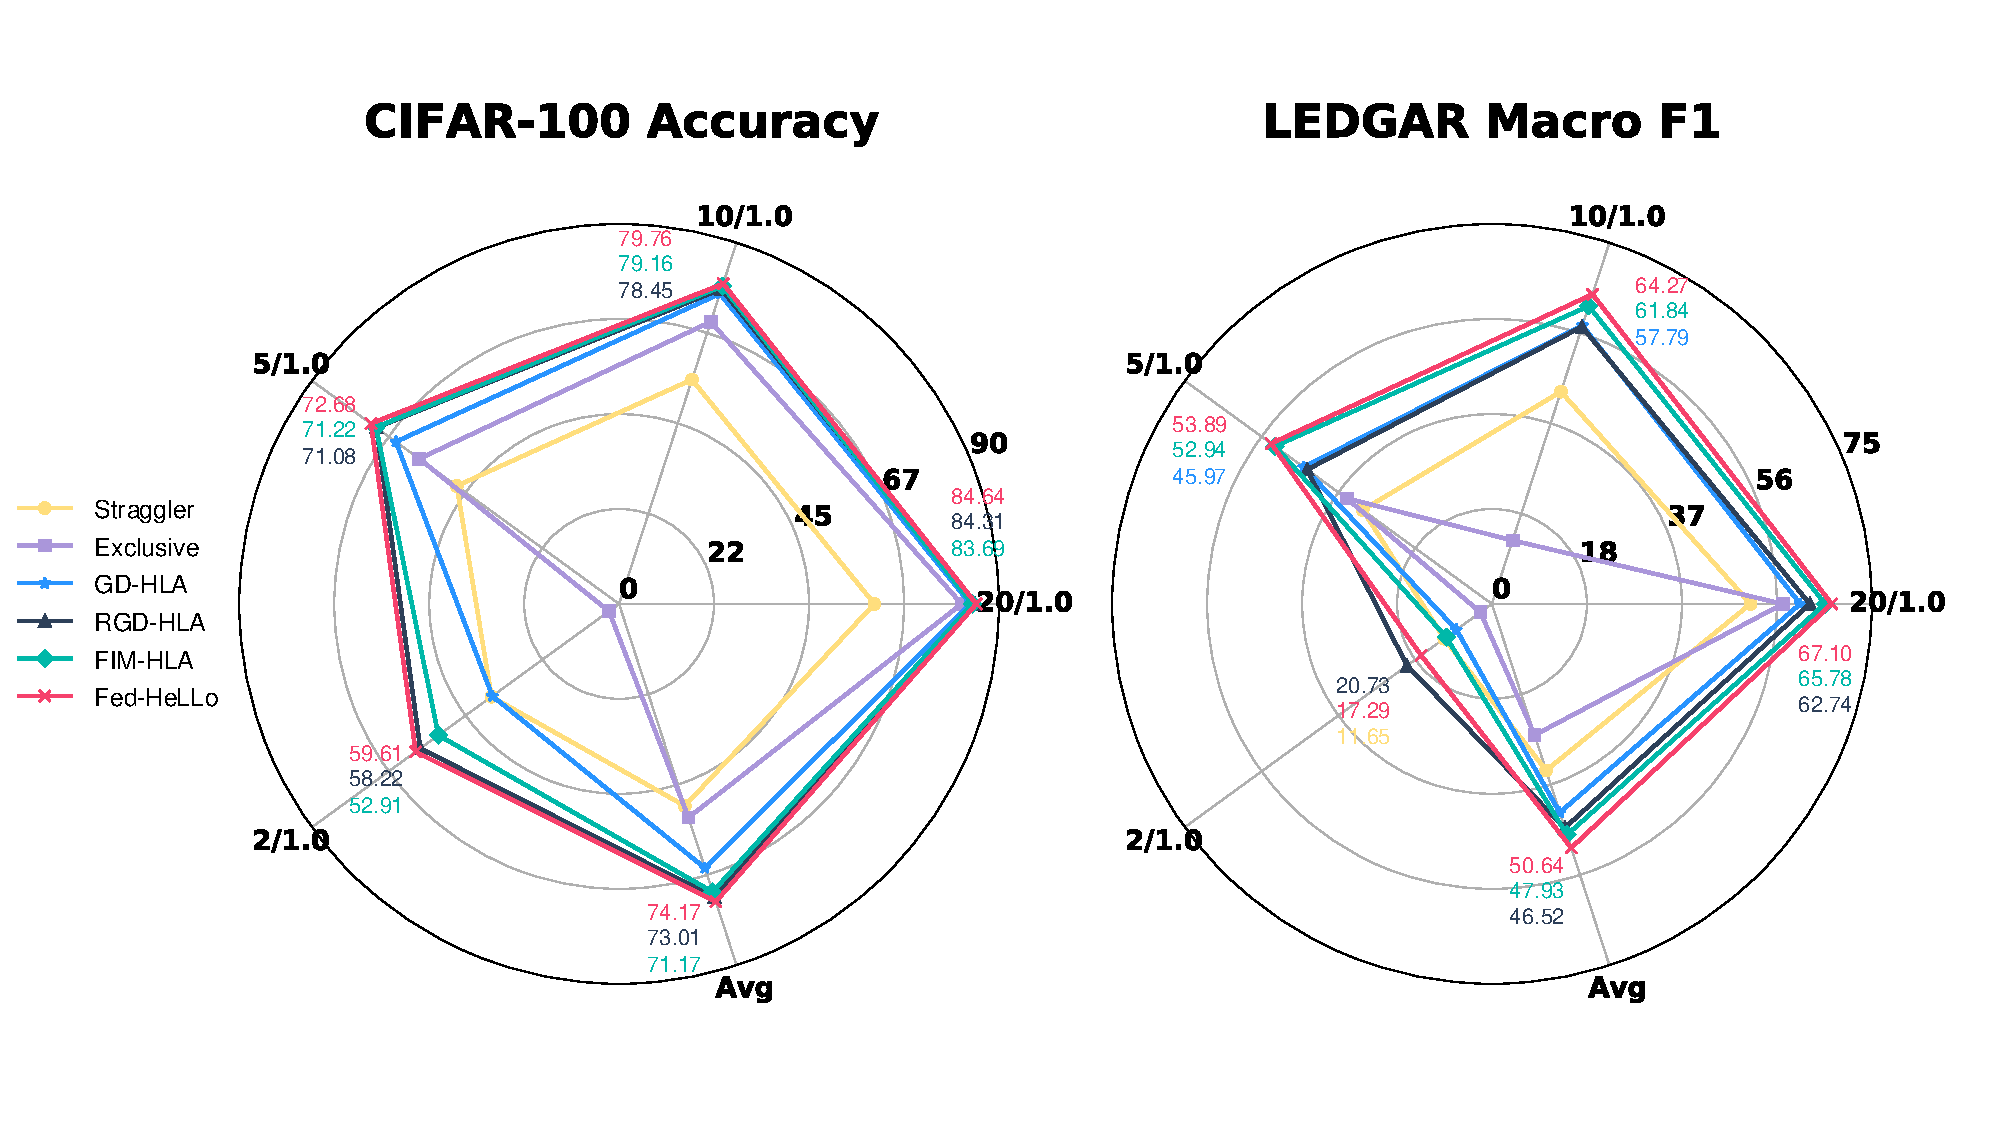
\includegraphics[width=0.9\linewidth]{figure/combined-radar-chart.pdf}
% \vspace*{-15pt}
\caption{The radar chart presents the results of the ablation study focused on evaluating the dynamic and intrinsic layer importance, specifically comparing our method with GD-HLA, RGD-HLA, FIM-HLA, and other baseline methods. The studies are conducted on both the CIFAR-100 and LEDGAR datasets, using 100 clients with a RoC distribution of 1:1:1. The Top-3 results for each spoke are listed near the vertices from top to bottom, with corresponding colors.}
\label{fig:importance-radar-chart}
% \vspace*{-10pt}
\end{figure}

In designing the Fed-HeLLo framework, we demonstrate that incorporating both dynamic and intrinsic layer importance can enhance model performance. Figure~\ref{fig:importance-radar-chart} presents two radar charts comparing the performance of GD-HLA, RGD-HLA, FIM-HLA, two baseline methods (i.e., Straggler and Exclusive Learning), and our method, with each method represented by different colored lines. The evaluation is conducted on two datasets, CIFAR-100 and LEDGAR. The radial axes display various data distribution settings and overall average performance, with each point representing a specific data distribution scenario or an aggregated result.

In the chart on the left, Fed-HeLLo (represented by the red line) consistently achieves high accuracy across all Non-IID settings, particularly excelling in the ``5/1.0'' and ``10/1.0'' settings, where it reaches 72.68\% and 79.76\%, respectively. It also leads in the ``20/1.0'' setting, achieving 84.64\% in accuracy. Compared to other methods, Straggler Learning (yellow) performs the worst, especially in the ``20/1.0'' setting, where its accuracy falls below 50\%. Exclusive Learning (purple) and GD-HLA (blue) demonstrate moderate performance, with GD-HLA slightly outperforming Exclusive Learning in most settings. RGD-HLA (black) and FIM-HLA (green) perform well but lag behind Fed-HeLLo in the more extreme Non-IID scenarios. The overall average accuracy further underscores the superiority of Fed-HeLLo, as it consistently surpasses other methods across different data heterogeneity levels.

In the chart on the right, Fed-HeLLo again demonstrates strong performance across Non-IID settings, especially in the ``10/1.0'' and ``20/1.0'' scenarios, where it achieves 64.27\% and 67.10\%, respectively. Straggler Learning continues to perform poorly, particularly in the ``2/1.0'' setting, where it falls to 11.65\%. Exclusive Learning and GD-HLA show moderate improvements over Straggler Learning, but they still fall short of Fed-HeLLo’s performance. {RGD-HLA exhibits competitive performance, especially in the ``10/1.0'' setting, which indicates the stable training is important for the extreme Non-IID cases.} The average F1 scores indicate that Fed-HeLLo is not only robust but also adaptable to varying degrees of client and data heterogeneity, maintaining high F1 scores across the board.
Across both datasets, Fed-HeLLo consistently outperforms the other methods in nearly every Non-IID setting, as well as in the overall average metrics, demonstrating its effectiveness in FL with heterogeneous clients.


% Table generated by Excel2LaTeX from sheet 'FIMSensitivity-ablation'
\begin{table}[t]
  \centering
  \caption{Justification of FIM-HLA with different training strategies.}
  \scalebox{1.05}{
    \begin{tabular}{c|cccc}
    \toprule[1pt]
    \textbf{Dataset/Model} & \multicolumn{4}{c}{\textbf{CIFAR-100/ViT-base}} \\
    \midrule
    \textbf{Metric} & \multicolumn{4}{c}{\textbf{Accuracy (\%)} $\uparrow$} \\
    \midrule
    \textbf{Methods/DH} & \textbf{IID} & \textbf{20/1.0} & \textbf{10/1.0} & \textbf{Avg} \\
    \midrule
    Proxy Data-1 & 84.02 & 77.27 & 69.95 & 77.08 \\
    Proxy Data-2 & 3.24  & 3.14  & 3.32  & 3.23 \\
    \textbf{Fed-HeLLo} & \cellcolor[rgb]{ .749,  .749,  .749}87.11 & \cellcolor[rgb]{ .749,  .749,  .749}84.64 & \cellcolor[rgb]{ .749,  .749,  .749}79.76 & \cellcolor[rgb]{ .749,  .749,  .749}79.03 \\
    \bottomrule[1pt]
    \end{tabular}%
    }
  \label{tab:abl-fim-1}%
\end{table}%

% Table generated by Excel2LaTeX from sheet 'FIMSensitivity-ablation'
\begin{table}[t]
  \centering
  \caption{Justification of FIM-HLA with Wikipedia proxy dataset.}
  \scalebox{1}{
    \begin{tabular}{c|cccc}
    \toprule[1pt]
    \textbf{Dataset/Model} & \multicolumn{4}{c}{\textbf{DomainNet121/ViT-base}} \\
    \midrule
    \textbf{Metric} & \multicolumn{4}{c}{\textbf{Accuracy (\%)} $\uparrow$} \\
    \midrule
    \textbf{Methods/DH} & \textbf{IID} & \textbf{25/1} & \textbf{15/1} & \textbf{Avg} \\
    \midrule
    HETLoRA & 64.26 & 48.92 & 35.34 & 49.50 \\
    FedRA & 68.53 & 55.64 & 51.07 & 58.41 \\
    \textbf{Fed-HeLLo-Wikipedia} & \cellcolor[rgb]{ .851,  .851,  .851}68.65 & \cellcolor[rgb]{ .851,  .851,  .851}57.74 & \cellcolor[rgb]{ .851,  .851,  .851}52.94 & \cellcolor[rgb]{ .851,  .851,  .851}59.78 \\
    \textbf{Fed-HeLLo} & \cellcolor[rgb]{ .749,  .749,  .749}68.98 & \cellcolor[rgb]{ .749,  .749,  .749}58.01 & \cellcolor[rgb]{ .749,  .749,  .749}53.74 & \cellcolor[rgb]{ .749,  .749,  .749}60.24 \\
    \bottomrule[1pt]
    \end{tabular}%
    }
  \label{tab:abl-fim-2}%
\end{table}%

\subsubsection{Justification of FIM-HLA}\label{subsubsec:fim-hla}
\textbf{Training Strategy:}
In FIM-HLA, we assume that the server holds a small proxy dataset. Ideally, the server could directly use this proxy dataset to improve the global model performance, making FIM-HLA unnecessary. To demonstrate that a small proxy dataset alone cannot significantly enhance fine-tuning performance and to justify the need for FIM-HLA, we conduct two additional experiments on CIFAR-100 dataset, named \textit{Proxy Data-1} and \textit{Proxy Data-2}. All experiments sample 10 out of 100 clients with a RoC of 1:1:1. In the first experiment, we implement Fed-HeLLo but with the server acting as an additional client with sufficient computational capability to fine-tune all LoRA layers using the proxy dataset. In the second experiment, we implement Fed-HeLLo but with the server using the proxy data to fine-tune the global model after aggregation at each round. The accuracy results for both experiments are reported in Table~\ref{tab:abl-fim-1}. 
% We observe that both proxy data-based global model fine-tuning methods result in a unfavorable performance, compared to FIM-HLA. These results show that the proxy dataset is insufficient for effective global model improvement, thus highlighting the necessity of applying FIM-HLA.
We observe that both proxy data-based global model fine-tuning methods result in unfavorable performance compared to FIM-HLA. 
For \textit{Proxy Data-1}, there are consistent performance drops compared to \textit{Fed-HeLLo}. This may be due to the server updates trained on proxy data being included in the model updates each round, causing the model to overfit to the proxy data and leading to suboptimal performance. 
For \textit{Proxy Data-2}, where the server fine-tunes the global model using proxy data after each aggregation round, the overfitting issue becomes even more severe, resulting in poor performance across all data distributions.
% These results show that the proxy dataset is insufficient for effective global model improvement, thus highlighting the necessity of applying FIM-HLA.
\textbf{Proxy Dataset from Wikipedia:} To further assess the sensitivity of the proxy data, we manually collect a dataset from Wikipedia\footnote{\url{https://www.wikipedia.org/}} for DomainNet-121 dataset. Specifically, we use each category name as a keyword, search for it on Wikipedia, and download the first image that appears, resulting in a small proxy dataset of 121 images (one per category). In Table~\ref{tab:abl-fim-2}, we present the experimental results using a 10/100 clients setting with a RoC of 1:1:1. For Fed-HeLLo, we use 1,000 random test data samples from DomainNet-121, which are excluded from all other training and evaluation. For Fed-HeLLo-Wikipedia, we utilize the proxy dataset collected from Wikipedia, following the same training conditions as Fed-HeLLo. In terms of results, Fed-HeLLo consistently outperforms all other methods across all scenarios, achieving the highest accuracy in the IID (68.98\%), 25/1 Non-IID (58.01\%), and 15/1 Non-IID (53.74\%) settings, with an overall average accuracy of 60.24\%. Fed-HeLLo-Wikipedia closely follows, particularly in the IID (68.65\%) and 25/1 Non-IID (57.74\%) settings, but with a slightly lower average accuracy of 59.78\%. This drop is possibly due to the proxy data from Wikipedia lacking domain diversity like DomainNet-121 and having fewer samples. FedRA falls behind in all scenarios, with an average accuracy of 58.41\%, while HETLoRA performs the worst, particularly in Non-IID scenarios, leading to the lowest overall average accuracy of 49.50\%.

\section{Limitations and Potential Future Works}\label{sec:limitation}
{\textbf{Privacy Preserving.} While our work leverages the inherent privacy-preserving nature of FL by ensuring that client data remains local and is not shared with the server or other clients, potential vulnerabilities still exist. For example, FL remains susceptible to privacy attacks such as model inversion~\cite{fredrikson2015model}, where adversaries attempt to reconstruct client data from model updates. Techniques like differential privacy~\cite{dwork2006differential} and secure aggregation~\cite{bonawitz2016practical} can be integrated into our framework to mitigate the vulnerability.}

{\textbf{Memory Constraint.} Additionally, the storage of intermediate activations is still challenging to resource-constrained clients. Activation saving techniques, such as sparsification~\cite{rao2021dynamicvit} and pruning~\cite{zhu2017prune}, can be integrated to reduce storage overhead while maintaining training stability. Future work can explore adaptive activation compression strategies to dynamically adjust compression levels based on available client resources, minimizing memory consumption without significantly impacting model performance.}

{\textbf{Training Process Improvement.} Furthermore, while Fed-HeLLo introduces HLA to reduce memory overhead, a better training process can be designed to improve the FL process. For example, model distillation~\cite{li2019fedmd} can be used to obtain a smaller FM for clients to reduce the storage burden.}

{\textbf{Data Heterogeneity.} While Fed-HeLLo effectively optimizes resource allocation through HLA, it does not directly address the challenge of data heterogeneity. 
% The presence of Non-IID data across clients can lead to significant variations in local model updates, making it difficult for the global model to achieve stable convergence. 
A potential future direction to mitigate the effects of data heterogeneity is to incorporate techniques such as federated feature alignment~\cite{yu2021fed2}, and adaptive weighting strategies~\cite{wu2021fast}.}

{By addressing these challenges, Fed-HeLLo can be further improved to enhance scalability, efficiency, and applicability in real-world FL scenarios.}


\section{Conclusion}
In this paper, we introduce Fed-HeLLo, a novel federated LoRA-based fine-tuning framework that integrates various HLA strategies.
These strategies allocate trainable LoRA layers based on clients' resource capabilities while considering both dynamic and intrinsic layer importance. 
To capture dynamic layer importance, we leverage FIM scores and design the FIM-HLA strategy. 
Additionally, to stabilize training in the early stages, 
% By incorporating both the dynamic and intrinsic layer importance, 
we propose GD-HLA and RGD-HLA strategies that account for intrinsic layer importance. By co-designing these strategies, Fed-HeLLo incorporates a comprehensive HLA design.
Extensive experiments on five LoRA-based fine-tuning datasets validate the effectiveness and efficiency of Fed-HeLLo, offering valuable insights for designing the HLA in FL with heterogeneous resource clients.

%%%%%%%%%%%%%%%%%%%%%%%%%%%%%%%%%%%%%%%%%%%%%%%%%%%%%%%%%%%%



{
\small
\bibliographystyle{plain}
\bibliography{ref.bib}
}


\vfill

\end{document}


